\chapter{Experimentation}
\label{chap:experiments}
This chapter deals with the experiments, their design, execution and results.

 
\section{Experimental Design}
This section deals the specification of the Android benchmark application, used hardware, frameworks, models and how the measurements are conducted. 
Figure \ref{fig:expDesign} depicts a brief overview of the design of the experiments, more precisely the used models, frameworks and hardware components, which are presented in greater detail in this section.
The role of the Android benchmark app is to emulate a AI application that delegates the inputs, which in our use case are images, to the edge or cloud inference framework for the inference process and gets the predictions as a response from the frameworks.

\begin{figure}[H]
\centering
\resizebox{.95\linewidth}{!}{

\tikzset{every picture/.style={line width=0.75pt}} %set default line width to 0.75pt        

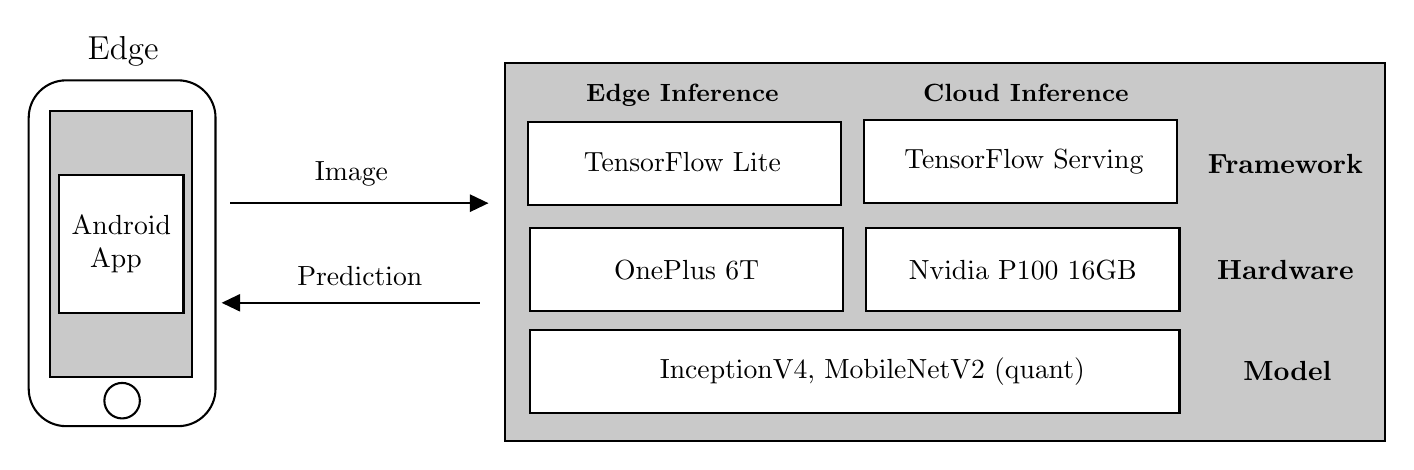
\begin{tikzpicture}[x=0.75pt,y=0.75pt,yscale=-1,xscale=1]
%uncomment if require: \path (0,485.57142639160156); %set diagram left start at 0, and has height of 485.57142639160156

%Straight Lines [id:da9993479608904674] 
\draw    (100.48,89) -- (223,89) ;
\draw [shift={(225,89)}, rotate = 540] [fill={rgb, 255:red, 0; green, 0; blue, 0 }  ][line width=0.75]  [draw opacity=0] (8.93,-4.29) -- (0,0) -- (8.93,4.29) -- cycle    ;

%Straight Lines [id:da5401559459790608] 
\draw    (98.48,137) -- (221,137) ;

\draw [shift={(96.48,137)}, rotate = 360] [fill={rgb, 255:red, 0; green, 0; blue, 0 }  ][line width=0.75]  [draw opacity=0] (8.93,-4.29) -- (0,0) -- (8.93,4.29) -- cycle    ;
%Shape: Rectangle [id:dp45054130026891115] 
\draw  [fill={rgb, 255:red, 201; green, 201; blue, 201 }  ,fill opacity=1 ] (233,21.57) -- (656.93,21.57) -- (656.93,203.57) -- (233,203.57) -- cycle ;
%Shape: Rectangle [id:dp21016153851852382] 
\draw  [fill={rgb, 255:red, 255; green, 255; blue, 255 }  ,fill opacity=1 ] (245,150) -- (557.93,150) -- (557.93,190) -- (245,190) -- cycle ;
%Shape: Rectangle [id:dp17739269402878732] 
\draw  [fill={rgb, 255:red, 255; green, 255; blue, 255 }  ,fill opacity=1 ] (244,50) -- (394.93,50) -- (394.93,90) -- (244,90) -- cycle ;
%Shape: Rectangle [id:dp9093436455970001] 
\draw  [fill={rgb, 255:red, 255; green, 255; blue, 255 }  ,fill opacity=1 ] (406,49) -- (556.93,49) -- (556.93,89) -- (406,89) -- cycle ;
%Shape: Rectangle [id:dp14120602080303146] 
\draw  [fill={rgb, 255:red, 255; green, 255; blue, 255 }  ,fill opacity=1 ] (245,101) -- (395.93,101) -- (395.93,141) -- (245,141) -- cycle ;
%Shape: Rectangle [id:dp45473714544487454] 
\draw  [fill={rgb, 255:red, 255; green, 255; blue, 255 }  ,fill opacity=1 ] (407,101) -- (557.93,101) -- (557.93,141) -- (407,141) -- cycle ;
%Shape: Rectangle [id:dp4153343207585154] 
\draw  [fill={rgb, 255:red, 201; green, 201; blue, 201 }  ,fill opacity=1 ] (13.91,44.69) -- (82.34,44.69) -- (82.34,172.63) -- (13.91,172.63) -- cycle ;
%Rounded Rect [id:dp09380596237315397] 
\draw   (3.5,47.82) .. controls (3.5,37.88) and (11.56,29.82) .. (21.5,29.82) -- (75.5,29.82) .. controls (85.44,29.82) and (93.5,37.88) .. (93.5,47.82) -- (93.5,178.43) .. controls (93.5,188.37) and (85.44,196.43) .. (75.5,196.43) -- (21.5,196.43) .. controls (11.56,196.43) and (3.5,188.37) .. (3.5,178.43) -- cycle ;
%Shape: Ellipse [id:dp8964060056788943] 
\draw   (39.95,184.16) .. controls (39.95,179.43) and (43.78,175.6) .. (48.5,175.6) .. controls (53.22,175.6) and (57.05,179.43) .. (57.05,184.16) .. controls (57.05,188.88) and (53.22,192.71) .. (48.5,192.71) .. controls (43.78,192.71) and (39.95,188.88) .. (39.95,184.16) -- cycle ;
%Shape: Rectangle [id:dp85708751067272] 
\draw  [fill={rgb, 255:red, 255; green, 255; blue, 255 }  ,fill opacity=1 ] (18.19,75.22) -- (78.07,75.22) -- (78.07,142.1) -- (18.19,142.1) -- cycle ;

% Text Node
\draw (159,75) node  [align=left] {Image};
% Text Node
\draw (163,124) node  [align=left] {Prediction};
% Text Node
\draw (49,16) node  [align=left] {{\large Edge}};
% Text Node
\draw (409.96,170) node  [align=left] {InceptionV4, MobileNetV2 (quant)};
% Text Node
\draw (318.46,37) node  [align=left] {{\small \textbf{Edge Inference}}};
% Text Node
\draw (483.96,36) node  [align=left] {{\small \textbf{Cloud Inference}}};
% Text Node
\draw (318.46,69) node  [align=left] {TensorFlow Lite};
% Text Node
\draw (482.96,68.79) node  [align=left] {TensorFlow Serving};
% Text Node
\draw (320.46,121) node  [align=left] {OnePlus 6T};
% Text Node
\draw (482.46,121) node  [align=left] {Nvidia P100 16GB};
% Text Node
\draw (608.96,70) node  [align=left] {\textbf{Framework}};
% Text Node
\draw (608.96,121) node  [align=left] {\textbf{Hardware}};
% Text Node
\draw (609.96,170) node  [align=left] {\textbf{Model}};
% Text Node
\draw (48.13,108.66) node  [align=left] {Android\\ \ \ App};


\end{tikzpicture}}
\caption{Experimental Design Architecture}
\label{fig:expDesign}
\end{figure}


\subsection{Hardware Devices}
\subsubsection{Edge}
\label{chap:hardwareEdge}
As the edge device we will use the OnePlus 6T (ONEPLUS A6013). This state of the art smartphone is powered by a Qualcomm Snapdragon 845 CPU(Octa-core, up to 2.8 GHz), Adreno 630 GPU, 8 GB of memory and runs on OxygenOS 9.0.11, which is based on Android 9.
%%Cite from AI bechmark paper
\subsubsection{Cloud}
%The Nvidia DGX-1 will serve as the cloud-backend for the experiments. This server consists of 8$\times$Tesla V100 providing 1000 TFLOPS as well as 256 GB GPU memory and 512 GB system memory.
We use a virtual server hosted at the LRZ, which has 32 cores (16 real cores with hyperthreading), 240 GB of memory, a Tesla P100 16 GB PCIe GPGPU and a 800 PCIe SSD.

The server runs on Ubuntu 16.04 CUDA 9.1 PGI 17.9 nvidia-docker 2.0.3+docker18.03.1-1.
\subsection{Deep Learning Inference Framework}
We use two open source machine learning frameworks, both based on TensorFlow, for the experiments, TensorFlow Lite and TensorFlow Serving. We decided to use these framework, because they are open source and support, at the point of this theses, most of the operations needed for the popular image classification models as well as an increasing number of hardware accelerators and operating systems for both edge and cloud inference.
TensorFlow provides official releases of deep learning models, that are well maintained and tested, including the ones we use in this thesis.

This section only gives a brief overview of the most important aspects of the frameworks, for detailed information consider the TensorFlow Lite\cite{tfLite}  and TensorFlow Serving\cite{tfServing} websites, on which this section is partly based on, or the corresponding GitHub repositories.
\subsubsection{TensorFlow Lite}
\label{chap:TFLite}
TensorFlow Lite (Release 1.12.0) was developed for mobile and embedded devices and is a lightweight solution of TensorFlow and thus will be used for the edge inference experiments.

%%Mention NNAPI support?
At the moment only model inference can be done by TensorFlow Lite, not model training.
It supports acceleration with GPU or other accelerators as well was portability to Android, iOS and other IoT devices.

\paragraph{Android NNAPI}
\label{chap:NNAPI}
TensorFlow Lite is also compatible with the Android Neural Networks API (NNAPI). This API
is designed to speed up computationally intensive machine learning operations and can be used by TensorFlow Lite to improve inference performance. During inference NNAPI "can
efficiently distribute the computation workload across available on-device processors, including dedicated neural network chips, GPUs and DSPs"\cite{DBLP:journals/corr/abs-1810-01109}.

Figure \ref{fig:NNAPIarchitecture} shows the architecture of the NNAPI. In our use case the application is our android benchmark application presented in section \ref{chap:androidApp} and the machine learning framework we use is TensorFlow Lite.
\begin{figure}[!htb]
\centering
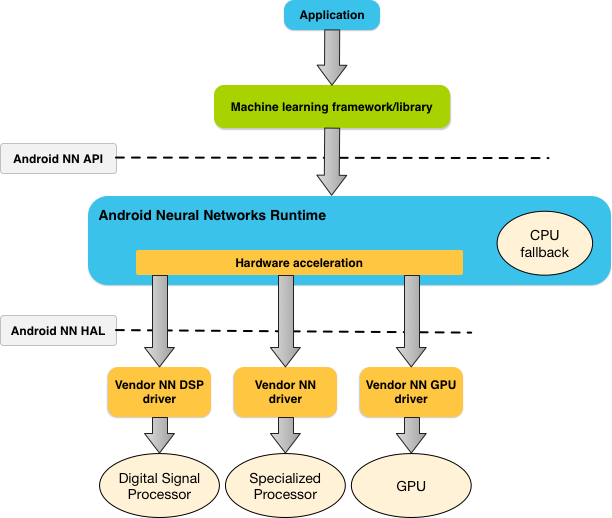
\includegraphics[width=0.5\textwidth]{./Bilder/nnapi_architecture.png}
\caption{System architecture for NNAPI framework \cite{NNAPI}}
\label{fig:NNAPIarchitecture}
\end{figure}


\paragraph{Hosting Models}
TensorFlow Lite expects models in their own \emph{FlatBuffer} file  format(\emph{.tflite}). Therefore models need to be converted to this format, before TensorFlow Lite can load them. This conversion can be done using the TensorFlow Lite Converter, which supports various formats of trained TensorFlow models.
After conversion a \emph{.tflite} model can be loaded by an object of the Interpreter class.
\paragraph{Run Prediction}

To then run the inference process in TensorFlow Lite the run method of Interpreter object with a loaded model needs to be called. To call this function two objects need to be passed, first the input for the given model and second the output object, where the prediction response from the inference operation get stored. 
\begin{figure}[H]
\centering



\tikzset{every picture/.style={line width=0.75pt}} %set default line width to 0.75pt        

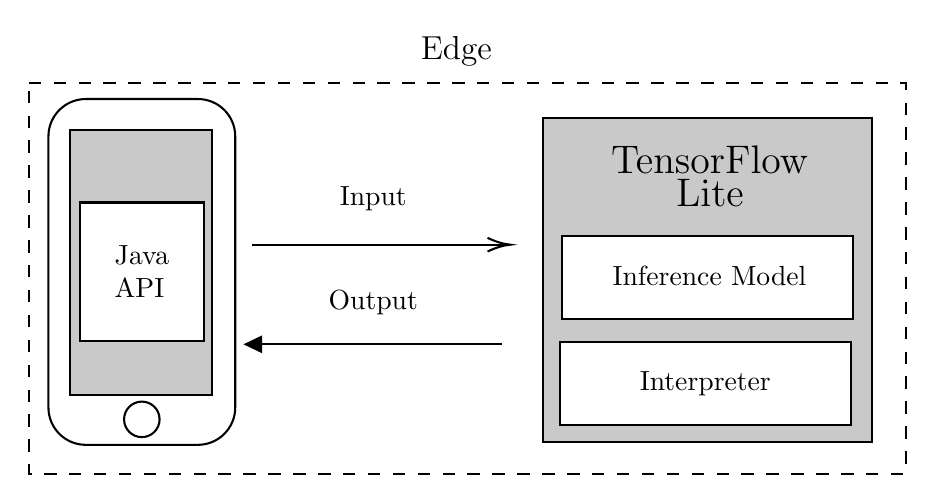
\begin{tikzpicture}[x=0.75pt,y=0.75pt,yscale=-1,xscale=1]
%uncomment if require: \path (0,300); %set diagram left start at 0, and has height of 300

%Shape: Rectangle [id:dp13292222689234756] 
\draw  [fill={rgb, 255:red, 201; green, 201; blue, 201 }  ,fill opacity=1 ] (61.91,111.69) -- (130.34,111.69) -- (130.34,239.63) -- (61.91,239.63) -- cycle ;
%Rounded Rect [id:dp7897713915001106] 
\draw   (51.5,114.82) .. controls (51.5,104.88) and (59.56,96.82) .. (69.5,96.82) -- (123.5,96.82) .. controls (133.44,96.82) and (141.5,104.88) .. (141.5,114.82) -- (141.5,245.43) .. controls (141.5,255.37) and (133.44,263.43) .. (123.5,263.43) -- (69.5,263.43) .. controls (59.56,263.43) and (51.5,255.37) .. (51.5,245.43) -- cycle ;
%Shape: Ellipse [id:dp9670901006981827] 
\draw   (87.95,251.16) .. controls (87.95,246.43) and (91.78,242.6) .. (96.5,242.6) .. controls (101.22,242.6) and (105.05,246.43) .. (105.05,251.16) .. controls (105.05,255.88) and (101.22,259.71) .. (96.5,259.71) .. controls (91.78,259.71) and (87.95,255.88) .. (87.95,251.16) -- cycle ;
%Straight Lines [id:da9993479608904674] 
\draw    (149.48,167) -- (272,167) ;
\draw [shift={(274,167)}, rotate = 540] [color={rgb, 255:red, 0; green, 0; blue, 0 }  ][line width=0.75]    (10.93,-3.29) .. controls (6.95,-1.4) and (3.31,-0.3) .. (0,0) .. controls (3.31,0.3) and (6.95,1.4) .. (10.93,3.29)   ;

%Straight Lines [id:da5401559459790608] 
\draw    (147.48,215) -- (270,215) ;

\draw [shift={(145.48,215)}, rotate = 360] [fill={rgb, 255:red, 0; green, 0; blue, 0 }  ][line width=0.75]  [draw opacity=0] (8.93,-4.29) -- (0,0) -- (8.93,4.29) -- cycle    ;
%Shape: Rectangle [id:dp45054130026891115] 
\draw  [fill={rgb, 255:red, 201; green, 201; blue, 201 }  ,fill opacity=1 ] (290,106) -- (448.5,106) -- (448.5,262) -- (290,262) -- cycle ;
%Shape: Rectangle [id:dp21016153851852382] 
\draw  [fill={rgb, 255:red, 255; green, 255; blue, 255 }  ,fill opacity=1 ] (299,163) -- (439,163) -- (439,203) -- (299,203) -- cycle ;
%Shape: Rectangle [id:dp8946256165796296] 
\draw  [fill={rgb, 255:red, 255; green, 255; blue, 255 }  ,fill opacity=1 ] (298,214) -- (438,214) -- (438,254) -- (298,254) -- cycle ;
%Shape: Rectangle [id:dp1345031923489386] 
\draw  [dash pattern={on 4.5pt off 4.5pt}] (42,89) -- (464.5,89) -- (464.5,277.4) -- (42,277.4) -- cycle ;
%Shape: Rectangle [id:dp7242946292477495] 
\draw  [fill={rgb, 255:red, 255; green, 255; blue, 255 }  ,fill opacity=1 ] (66.56,146.69) -- (126.44,146.69) -- (126.44,213.56) -- (66.56,213.56) -- cycle ;

% Text Node
\draw (208,145) node  [align=left] {Input};
% Text Node
\draw (248,74) node  [align=left] {{\large Edge}};
% Text Node
\draw (370,134) node  [align=left] {{\Large TensorFlow}\\{\Large  \ \ \ \ \ Lite}};
% Text Node
\draw (370,182) node  [align=left] {Inference Model};
% Text Node
\draw (208,195) node  [align=left] {Output};
% Text Node
\draw (368,234) node  [align=left] {Interpreter};
% Text Node
\draw (96.5,180.12) node  [align=left] {Java\\ API};


\end{tikzpicture}
\caption{Functionality of TensorFlow Lite}
\label{fig:edge}
\end{figure}
\subsubsection{TensorFlow Serving}
\label{chap:TFServing}
TensorFlow Serving (Release 1.12.0 VERIFY THIS AGAIN) will be used as the cloud inference framework, since it provides a framework to serve machine learning models in production environments. 



\paragraph{Hosting Models}
In order to host a model as a Servable in TensorFlow Serving, first a TensorFlow model needs to exported using TensorFlow's \emph{SavedModelBuilder}, resulting in a \emph{SavedModel protocol} buffer file along with the model’s variables and assets (Although TensorFlow Serving is optimized for TensorFlow models, the framework can be extended to serve other types of models).
%%Wieviel schreiben über signature, predict function etc?

Now the exported model can be loaded by a instance of Tensorflow Serving.
We use docker to start that instance, specifically nvidia-docker that allows us to run the inference operations on a GPU. For that TensorFlow Serving provides two docker images of their framework, one with CPU and the other with GPU support.

\paragraph{Run Prediction}
TensorFlow Serving supports two API for clients to create predictions requests: gRPC and REST. Since the gRPC protocol is supposed to deliver a better performance in the form of lower latencies and smaller payloads, we will use the gRPC API in this thesis.
Before a client can make a resquest to the server, a gRPC stub needs to be created in the first place, that allows us to call all methods implemented on the server. In our case we need to call TensorFlow Serving's \emph{Predict} method to start the inference process. The method needs to be passed a \emph{PredictRequest} object, which contains among other things the input data for the model, the shape of the input and the requested model.%model signature?

After the request is sent and handled the server response by sending back a \emph{PredictResponse} object. This object holds the predictions for the given input data in the form specified by the exported model.
This request and response process can also be seen in figure \ref{fig:cloud}

\begin{figure}[H]
\centering


\tikzset{every picture/.style={line width=0.75pt}} %set default line width to 0.75pt        

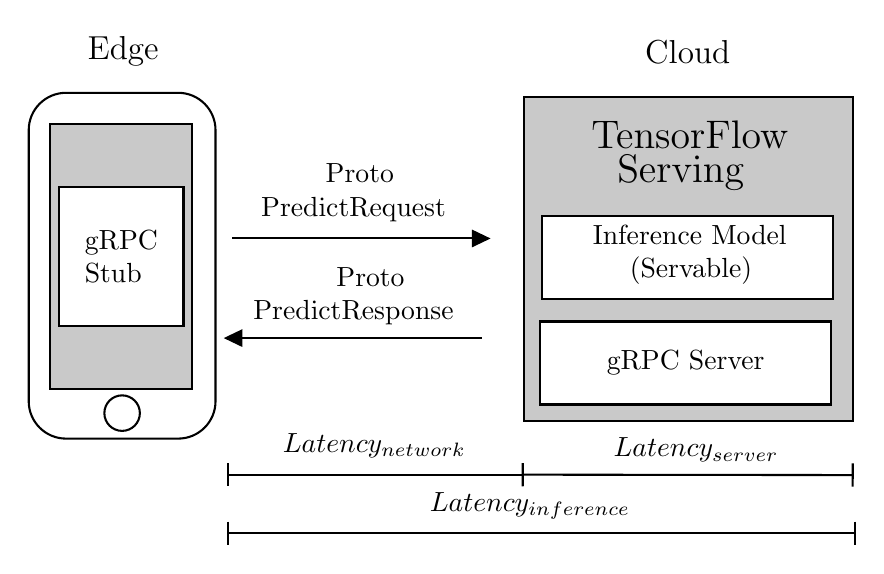
\begin{tikzpicture}[x=0.75pt,y=0.75pt,yscale=-1,xscale=1]
%uncomment if require: \path (0,300); %set diagram left start at 0, and has height of 300

%Straight Lines [id:da7072764839644827] 
\draw    (149.5,291) -- (451.5,291) ;
\draw [shift={(451.5,291)}, rotate = 180] [color={rgb, 255:red, 0; green, 0; blue, 0 }  ][line width=0.75]    (0,5.59) -- (0,-5.59)   ;
\draw [shift={(149.5,291)}, rotate = 180] [color={rgb, 255:red, 0; green, 0; blue, 0 }  ][line width=0.75]    (0,5.59) -- (0,-5.59)   ;
%Straight Lines [id:da9536138531960994] 
\draw    (291.5,262.8) -- (450.5,263) ;
\draw [shift={(450.5,263)}, rotate = 180.07] [color={rgb, 255:red, 0; green, 0; blue, 0 }  ][line width=0.75]    (0,5.59) -- (0,-5.59)   ;
\draw [shift={(291.5,262.8)}, rotate = 180.07] [color={rgb, 255:red, 0; green, 0; blue, 0 }  ][line width=0.75]    (0,5.59) -- (0,-5.59)   ;
%Shape: Rectangle [id:dp8902536871651789] 
\draw  [fill={rgb, 255:red, 201; green, 201; blue, 201 }  ,fill opacity=1 ] (63.91,93.69) -- (132.34,93.69) -- (132.34,221.63) -- (63.91,221.63) -- cycle ;
%Rounded Rect [id:dp41557214204551274] 
\draw   (53.5,96.82) .. controls (53.5,86.88) and (61.56,78.82) .. (71.5,78.82) -- (125.5,78.82) .. controls (135.44,78.82) and (143.5,86.88) .. (143.5,96.82) -- (143.5,227.43) .. controls (143.5,237.37) and (135.44,245.43) .. (125.5,245.43) -- (71.5,245.43) .. controls (61.56,245.43) and (53.5,237.37) .. (53.5,227.43) -- cycle ;
%Shape: Ellipse [id:dp8878397246816687] 
\draw   (89.95,233.16) .. controls (89.95,228.43) and (93.78,224.6) .. (98.5,224.6) .. controls (103.22,224.6) and (107.05,228.43) .. (107.05,233.16) .. controls (107.05,237.88) and (103.22,241.71) .. (98.5,241.71) .. controls (93.78,241.71) and (89.95,237.88) .. (89.95,233.16) -- cycle ;
%Straight Lines [id:da5813802620369573] 
\draw    (151.48,149) -- (274,149) ;
\draw [shift={(276,149)}, rotate = 540] [fill={rgb, 255:red, 0; green, 0; blue, 0 }  ][line width=0.75]  [draw opacity=0] (8.93,-4.29) -- (0,0) -- (8.93,4.29) -- cycle    ;

%Straight Lines [id:da16220168680973557] 
\draw    (149.48,197) -- (272,197) ;

\draw [shift={(147.48,197)}, rotate = 360] [fill={rgb, 255:red, 0; green, 0; blue, 0 }  ][line width=0.75]  [draw opacity=0] (8.93,-4.29) -- (0,0) -- (8.93,4.29) -- cycle    ;
%Shape: Rectangle [id:dp8411150472244695] 
\draw  [fill={rgb, 255:red, 201; green, 201; blue, 201 }  ,fill opacity=1 ] (292,81) -- (450.5,81) -- (450.5,237) -- (292,237) -- cycle ;
%Shape: Rectangle [id:dp13557861576626729] 
\draw  [fill={rgb, 255:red, 255; green, 255; blue, 255 }  ,fill opacity=1 ] (301,138) -- (441,138) -- (441,178) -- (301,178) -- cycle ;
%Shape: Rectangle [id:dp5681963435258506] 
\draw  [fill={rgb, 255:red, 255; green, 255; blue, 255 }  ,fill opacity=1 ] (68.19,124.22) -- (128.07,124.22) -- (128.07,191.1) -- (68.19,191.1) -- cycle ;
%Shape: Rectangle [id:dp7458124222136935] 
\draw  [fill={rgb, 255:red, 255; green, 255; blue, 255 }  ,fill opacity=1 ] (300,189) -- (440,189) -- (440,229) -- (300,229) -- cycle ;
%Straight Lines [id:da6846625455377753] 
\draw    (149.5,262.8) -- (291.5,262.8) ;
\draw [shift={(291.5,262.8)}, rotate = 180] [color={rgb, 255:red, 0; green, 0; blue, 0 }  ][line width=0.75]    (0,5.59) -- (0,-5.59)   ;
\draw [shift={(149.5,262.8)}, rotate = 180] [color={rgb, 255:red, 0; green, 0; blue, 0 }  ][line width=0.75]    (0,5.59) -- (0,-5.59)   ;

% Text Node
\draw (375,251) node  [align=left] {$\displaystyle Latency_{server}$$ $};
% Text Node
\draw (210,127) node  [align=left] { \ \ \ \ \ \ \ Proto\\PredictRequest};
% Text Node
\draw (99,59) node  [align=left] {{\large Edge}};
% Text Node
\draw (371,59) node  [align=left] {{\large Cloud}};
% Text Node
\draw (372,109) node  [align=left] {{\Large TensorFlow}\\{\Large  \ \ Serving}};
% Text Node
\draw (372,157) node  [align=left] {Inference Model\\ \ \ \ \ (Servable)};
% Text Node
\draw (210,177) node  [align=left] { \ \ \ \ \ \ \ \ \ Proto\\PredictResponse};
% Text Node
\draw (98.13,157.66) node  [align=left] {gRPC\\ Stub};
% Text Node
\draw (370,209) node  [align=left] {gRPC Server};
% Text Node
\draw (220,249) node  [align=left] {$\displaystyle Latency_{network}$$ $};
% Text Node
\draw (295,278) node  [align=left] {$\displaystyle Latency_{inference}$$ $};


\end{tikzpicture}
\caption{Basic Functionality of TensorFlow Serving}
\label{fig:cloud}
\end{figure}
\subsection{Models}
\label{chap:models}
We will benchmark two different image classification models in this thesis, MobileNetV2 and InceptionV4, the first is optimized for mobile deployment and the second towards high accuracy.
Both models are trained on a ImageNet dataset consisting of 1001 image classes (1000 image classes + 1 class for other image classes).
An overview of the models can be seen in table \ref{table:modelOverview} in the form of top-5 accuracy (a prediction is classified as accurate if the five labels with the highest confidence contain the real class of the input image), the input size of the model, the number of parameters in millions and the model size in the TensorFlow Lite format.
InceptionV4 has $4.5\%$ more accuracy than MobileNetV2, but also more than $12$ times more parameters and $7.5$ times larger TensorFlow Lite model size.
MobileNetV2 also uses a smaller input sizes of $224\times224$ than InceptionV4's $299\times299$ input size.
\begin{table}[H]
%CITE inception params ned vergessen
%http://dgschwend.github.io/netscope/#/preset/inceptionv4
\caption{Overview of used models}
\label{table:modelOverview}
\begin{tabular}{@{}lllll@{}}
\toprule
Model & Parameters & Top-5 Accuracy\cite{modelspecs} & Input Size & TF Lite Model Size \\
\midrule
InceptionV4 & $42.68$M & $95.1\%$ & $299\times299$ & $107.7$MB \\
MobileNetV2 1.0 & $3.47$M\cite{DBLP:journals/corr/abs-1801-04381} & $90.6\%$ & $224\times224$ & $14$MB \\
\begin{tabular}[c]{@{}l@{}}MobileNetV2 1.0\\quantized\end{tabular}  & $3.47$M\cite{DBLP:journals/corr/abs-1801-04381} & $89.9\%$ & $224\times224$ & $3.4$MB\\
\bottomrule
\end{tabular}
\end{table}
For the TensorFlow Lite version we use the models provided on the TensorFlow Lite website \cite{tfLiteModels}.
To convert model suitable for TensorFlow Serving, we use the TensorFlow-Slim library \cite{tfSlim}, where maintained and tested implementations of popular image classification models are being published. For both Serving and Lite we use the same training checkpoint to get the same weights for the graphs.

In the following we give a brief overview of the models, their unique building blocks and the intuition behind them.
For full details please refer to \cite{DBLP:journals/corr/abs-1801-04381} and \cite{InceptionV4}.

\subsubsection{MobileNetV2}
MobileNetV2 (version 1.0) is a successor of MobileNetV1 and is "specifically tailored for mobile and resource
constrained environments" \cite{DBLP:journals/corr/abs-1801-04381}. The authors do this by "significantly decreasing the number of operations and the memory needed while retaining the same accuracy"  \cite{DBLP:journals/corr/abs-1801-04381} and introducing a new layer module called "the
inverted residual with linear bottleneck".

This module is visualized in figure \ref{fig:bottleneckBlock} and consists of two parts: The inverted residual block and a shortcut from the input to the output.
In a first step of the inverted residual block the channel dimension of the input are expanded with the use of a pointwise $1\times1$ convolution layer. 
Afterwards depthwise $3\times3$ convolution is applied to the expanded input. Then again a pointwise $1\times1$ convolution gets used, but this time the dimensions are decreased instead of increased.

The intuition behind this module is that the expansion decodes information ensuring that the features can be extracted during the depthwise convolution. The extracted features then get encoded again by reducing the dimensions.
To improve the backpropagation of the gradient across multiple layers during the training the authors add the shortcut to the module, resulting in faster training and better accuracy.
The bottleneck module can be implemented very memory efficient, thus particularly fit for edge inference.

Figure \ref{fig:MobileNetArchi} displays the overall architecture of the model, with the majority of the building blocks being the bottleneck modules.
All bottleneck modules in a sequence have the same number of output channels and use a stride of $1$, except for the first bottleneck block in a sequence. All spatial convolutions use $3\times3$ kernels. 
Although not depicted on the figure, the model uses dropout and batch normalization during training.
%%expanstionf actor?
%%$$shortcut!! expanded by a "expansion factor" varying for different seqences

\begin{figure}[!htb]
\centering
   \resizebox{.7\linewidth}{!}{

\tikzset{every picture/.style={line width=0.75pt}} %set default line width to 0.75pt        

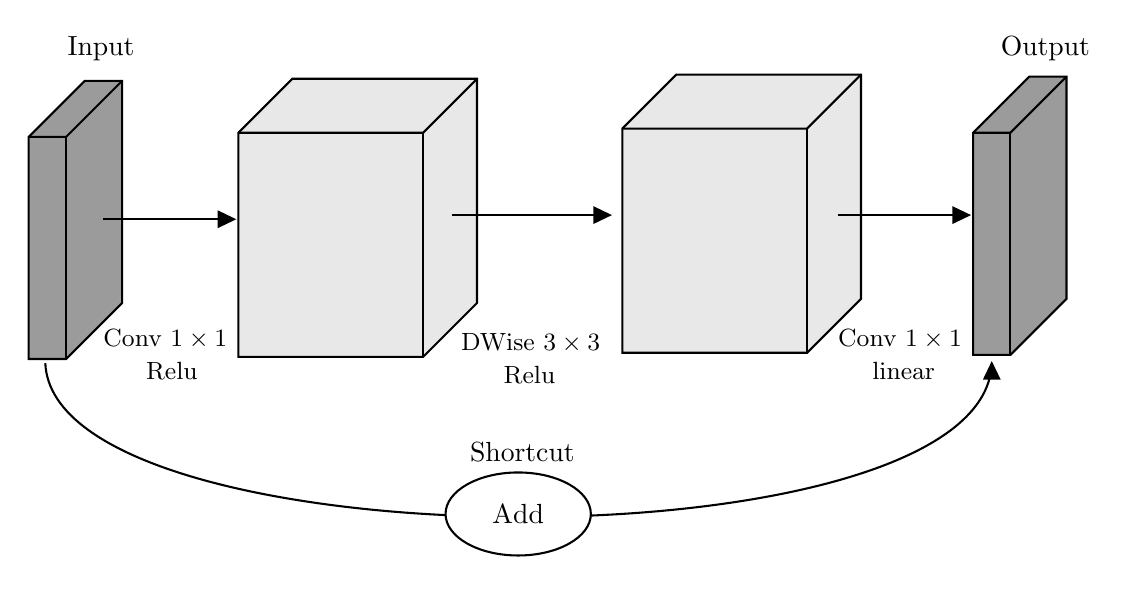
\begin{tikzpicture}[x=0.75pt,y=0.75pt,yscale=-1,xscale=1]
%uncomment if require: \path (0,600); %set diagram left start at 0, and has height of 600

%Shape: Cube [id:dp0950450187441989] 
\draw  [fill={rgb, 255:red, 155; green, 155; blue, 155 }  ,fill opacity=1 ] (24.17,60.33) -- (51.17,33.33) -- (69.17,33.33) -- (69.17,140.33) -- (42.17,167.33) -- (24.17,167.33) -- cycle ; \draw   (69.17,33.33) -- (42.17,60.33) -- (24.17,60.33) ; \draw   (42.17,60.33) -- (42.17,167.33) ;
%Shape: Cube [id:dp5388410753431343] 
\draw  [fill={rgb, 255:red, 155; green, 155; blue, 155 }  ,fill opacity=1 ] (479.17,58.33) -- (506.17,31.33) -- (524.17,31.33) -- (524.17,138.33) -- (497.17,165.33) -- (479.17,165.33) -- cycle ; \draw   (524.17,31.33) -- (497.17,58.33) -- (479.17,58.33) ; \draw   (497.17,58.33) -- (497.17,165.33) ;
%Shape: Cube [id:dp5352049268129733] 
\draw  [fill={rgb, 255:red, 232; green, 232; blue, 232 }  ,fill opacity=1 ] (125.17,58.33) -- (151.17,32.33) -- (240.17,32.33) -- (240.17,140.33) -- (214.17,166.33) -- (125.17,166.33) -- cycle ; \draw   (240.17,32.33) -- (214.17,58.33) -- (125.17,58.33) ; \draw   (214.17,58.33) -- (214.17,166.33) ;
%Shape: Cube [id:dp5972901431854747] 
\draw  [fill={rgb, 255:red, 232; green, 232; blue, 232 }  ,fill opacity=1 ] (310.17,56.33) -- (336.17,30.33) -- (425.17,30.33) -- (425.17,138.33) -- (399.17,164.33) -- (310.17,164.33) -- cycle ; \draw   (425.17,30.33) -- (399.17,56.33) -- (310.17,56.33) ; \draw   (399.17,56.33) -- (399.17,164.33) ;
%Curve Lines [id:da4213776555105224] 
\draw    (32.17,169.33) .. controls (36.15,266.84) and (483.66,269.31) .. (488.13,169.84) ;
\draw [shift={(488.17,168.33)}, rotate = 450] [fill={rgb, 255:red, 0; green, 0; blue, 0 }  ][line width=0.75]  [draw opacity=0] (8.93,-4.29) -- (0,0) -- (8.93,4.29) -- cycle    ;

%Straight Lines [id:da7525961556824932] 
\draw    (60,100) -- (122.17,100) ;
\draw [shift={(124.17,100)}, rotate = 180] [fill={rgb, 255:red, 0; green, 0; blue, 0 }  ][line width=0.75]  [draw opacity=0] (8.93,-4.29) -- (0,0) -- (8.93,4.29) -- cycle    ;

%Straight Lines [id:da7778926134720376] 
\draw    (228,98) -- (303.17,98) ;
\draw [shift={(305.17,98)}, rotate = 180] [fill={rgb, 255:red, 0; green, 0; blue, 0 }  ][line width=0.75]  [draw opacity=0] (8.93,-4.29) -- (0,0) -- (8.93,4.29) -- cycle    ;

%Straight Lines [id:da2814517292192529] 
\draw    (414,98) -- (476.17,98) ;
\draw [shift={(478.17,98)}, rotate = 180] [fill={rgb, 255:red, 0; green, 0; blue, 0 }  ][line width=0.75]  [draw opacity=0] (8.93,-4.29) -- (0,0) -- (8.93,4.29) -- cycle    ;

%Shape: Ellipse [id:dp8668947513316778] 
\draw  [fill={rgb, 255:red, 255; green, 255; blue, 255 }  ,fill opacity=1 ] (225,242) .. controls (225,230.95) and (240.67,222) .. (260,222) .. controls (279.33,222) and (295,230.95) .. (295,242) .. controls (295,253.05) and (279.33,262) .. (260,262) .. controls (240.67,262) and (225,253.05) .. (225,242) -- cycle ;

% Text Node
\draw (262,212) node  [align=left] {Shortcut};
% Text Node
\draw (90,165) node  [align=left] {{\small Conv $\displaystyle 1\times 1$}\\{\small  \ \ \ \ \ Relu}};
% Text Node
\draw (266,167) node  [align=left] {{\small DWise $\displaystyle 3\times 3$}\\{\small  \ \ \ \ \ Relu}};
% Text Node
\draw (444,165) node  [align=left] {{\small Conv $\displaystyle 1\times 1$}\\{\small  \ \ \ \ linear}};
% Text Node
\draw (260,242) node  [align=left] {Add};
% Text Node
\draw (59,18) node  [align=left] {Input};
% Text Node
\draw (514,18) node  [align=left] {Output};


\end{tikzpicture}}
\caption{Inverted Residual Block (bottleneck)}
\label{fig:bottleneckBlock}
%%NO DROPOUT AT INFERENCE
\end{figure}


\begin{comment}


\begin{table}[]

\centering
\caption{MobilenetV2 architecture \cite{DBLP:journals/corr/abs-1801-04381}}
\label{table:mobilenetArchi}
\begin{tabular}{@{}llllll@{}}

\toprule
Input & Operator & t & c & n & s \\ \midrule
$224^2\times 3$ & conv2d & - & 32 & 1 & 2 \\
$112^2\times 32$ & bottleneck & 1 & 16 & 1 & 1 \\
$112^2\times 16$ & bottleneck & 6 & 24 & 2 & 2 \\
$56^2\times 24$ & bottleneck & 6 & 32 & 3 & 2 \\
$28^2\times 23$ & bottleneck & 6 & 64 & 4 & 2 \\
$14^2\times 64$ & bottleneck & 6 & 96 & 3 & 1 \\
$14^2\times 96$ & bottleneck & 6 & 160 & 3 & 2 \\
$7^2\times 160$ & bottleneck & 6 & 320 & 1 & 1 \\
$7^2\times 320$ & conv2d 1x1 & - & 1280 & 1 & 1 \\
$7^2\times 1280$ & avgpool 7x7 & - & - & 1 & - \\
$1\times 1\times 1280$ & conv2d 1x1 & - & k & - &  \\ \bottomrule
\end{tabular}
\end{table}
\end{comment}
\paragraph{Quantization}
Quantization of MobileNetV2, using the techniques presented in section \ref{chap:quant}, results in a  0.7\% loss of top-5 accuracy, but therefore has lost 75\% of its model size (see table \ref{table:modelOverview}) and is supposed to deliver a better inference performance, which we will evaluate in the experiments.



\subsubsection{Inception V4}
%%Add infos about stem and reduction
InceptionV4, published in \cite{InceptionV4}, is a large image classification network with high accuracy, but also with a high number of parameters leading to higher computational demands than MobileNetV2 and thus larger impact on inference performance.
In comparison to its previous versions InceptionV4 is built with "a more uniform simplified architecture and more inception modules". 

The general architecture of the network can be seen in figure \ref{fig:inceptionv4Archi} with the fundamental building blocks being multiple Inception (A-C) and Reduction(A-B) modules. 
An example for both of these modules can be seen in figures \ref{fig:InceptionA} and \ref{fig:InceptionReduction}.
Inception modules are built of multiple convolutions with multiple filters and pooling layers in parallel within the same layer.
After the convolutions the output of all convolutions are concatenated.
The intuition behind this parallelism is to give the model multiple convolution choices for a given input and let the model learn itself the best feature extractor. An additional benefit is that the model can extract both local and more complex feature from an input.

To reduce the dimensionality before computational expensive large convolutions, and thus speed up training, the authors introduce the Reduction block containing small $1\times1$ convolutions.   %genauer erklären




\begin{figure}[!htb]
\centering
\begin{subfigure}[b]{.95\textwidth}
\centering
   \resizebox{.8\linewidth}{!}{

\tikzset{every picture/.style={line width=0.75pt}} %set default line width to 0.75pt        

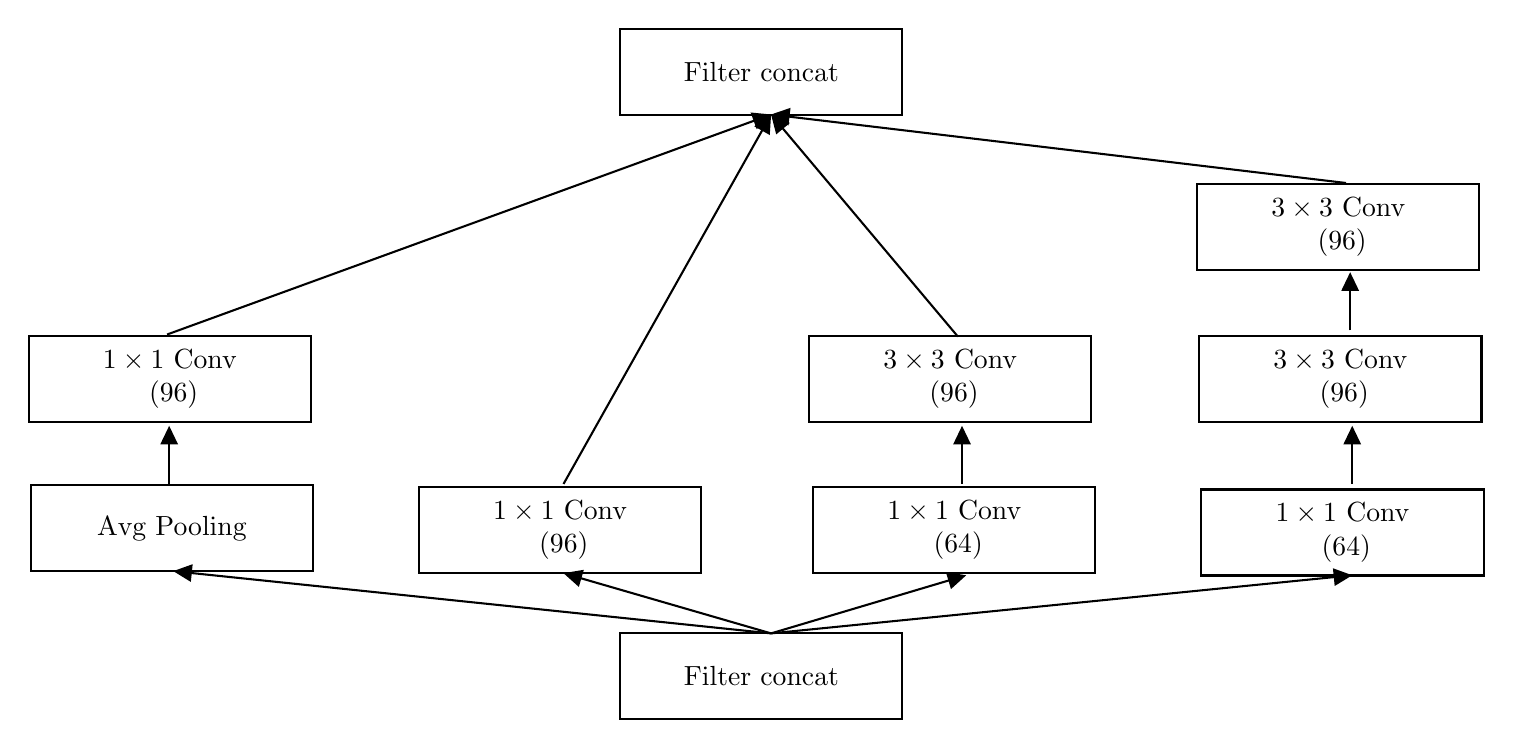
\begin{tikzpicture}[x=0.75pt,y=0.75pt,yscale=-1,xscale=1]
%uncomment if require: \path (0,550.3333358764648); %set diagram left start at 0, and has height of 550.3333358764648

%Flowchart: Process [id:dp8446713243434529] 
\draw   (508,479) -- (643.93,479) -- (643.93,520.43) -- (508,520.43) -- cycle ;
%Flowchart: Process [id:dp8389212433494444] 
\draw   (224,408) -- (359.93,408) -- (359.93,449.43) -- (224,449.43) -- cycle ;
%Flowchart: Process [id:dp9696039225192121] 
\draw   (411,409) -- (546.93,409) -- (546.93,450.43) -- (411,450.43) -- cycle ;
%Flowchart: Process [id:dp31126408548780393] 
\draw   (601,409) -- (736.93,409) -- (736.93,450.43) -- (601,450.43) -- cycle ;
%Flowchart: Process [id:dp739948518816423] 
\draw   (788,410) -- (923.93,410) -- (923.93,451.43) -- (788,451.43) -- cycle ;
%Straight Lines [id:da20227844614554824] 
\draw    (580.67,479.33) -- (294.66,449.54) ;
\draw [shift={(292.67,449.33)}, rotate = 365.95] [fill={rgb, 255:red, 0; green, 0; blue, 0 }  ][line width=0.75]  [draw opacity=0] (8.93,-4.29) -- (0,0) -- (8.93,4.29) -- cycle    ;

%Straight Lines [id:da9079516459586603] 
\draw    (580.67,479.33) -- (482.59,450.89) ;
\draw [shift={(480.67,450.33)}, rotate = 376.16999999999996] [fill={rgb, 255:red, 0; green, 0; blue, 0 }  ][line width=0.75]  [draw opacity=0] (8.93,-4.29) -- (0,0) -- (8.93,4.29) -- cycle    ;

%Straight Lines [id:da7697048902828942] 
\draw    (580.67,479.33) -- (672.75,451.9) ;
\draw [shift={(674.67,451.33)}, rotate = 523.4100000000001] [fill={rgb, 255:red, 0; green, 0; blue, 0 }  ][line width=0.75]  [draw opacity=0] (8.93,-4.29) -- (0,0) -- (8.93,4.29) -- cycle    ;

%Straight Lines [id:da004295071242706339] 
\draw    (580.67,479.33) -- (858.68,451.53) ;
\draw [shift={(860.67,451.33)}, rotate = 534.29] [fill={rgb, 255:red, 0; green, 0; blue, 0 }  ][line width=0.75]  [draw opacity=0] (8.93,-4.29) -- (0,0) -- (8.93,4.29) -- cycle    ;

%Flowchart: Process [id:dp6126721254059377] 
\draw   (223,336) -- (358.93,336) -- (358.93,377.43) -- (223,377.43) -- cycle ;
%Flowchart: Process [id:dp6415327260036892] 
\draw   (599,336) -- (734.93,336) -- (734.93,377.43) -- (599,377.43) -- cycle ;
%Flowchart: Process [id:dp557242506777897] 
\draw   (787,336) -- (922.93,336) -- (922.93,377.43) -- (787,377.43) -- cycle ;
%Flowchart: Process [id:dp895045490145193] 
\draw   (786,263) -- (921.93,263) -- (921.93,304.43) -- (786,304.43) -- cycle ;
%Straight Lines [id:da042686267300120706] 
\draw    (290.67,407.33) -- (290.67,381.33) ;
\draw [shift={(290.67,379.33)}, rotate = 450] [fill={rgb, 255:red, 0; green, 0; blue, 0 }  ][line width=0.75]  [draw opacity=0] (8.93,-4.29) -- (0,0) -- (8.93,4.29) -- cycle    ;

%Straight Lines [id:da1451751743173857] 
\draw    (672.67,407.33) -- (672.67,381.33) ;
\draw [shift={(672.67,379.33)}, rotate = 450] [fill={rgb, 255:red, 0; green, 0; blue, 0 }  ][line width=0.75]  [draw opacity=0] (8.93,-4.29) -- (0,0) -- (8.93,4.29) -- cycle    ;

%Straight Lines [id:da7065201039263691] 
\draw    (860.67,407.33) -- (860.67,381.33) ;
\draw [shift={(860.67,379.33)}, rotate = 450] [fill={rgb, 255:red, 0; green, 0; blue, 0 }  ][line width=0.75]  [draw opacity=0] (8.93,-4.29) -- (0,0) -- (8.93,4.29) -- cycle    ;

%Straight Lines [id:da3529249322466719] 
\draw    (859.67,333.33) -- (859.67,307.33) ;
\draw [shift={(859.67,305.33)}, rotate = 450] [fill={rgb, 255:red, 0; green, 0; blue, 0 }  ][line width=0.75]  [draw opacity=0] (8.93,-4.29) -- (0,0) -- (8.93,4.29) -- cycle    ;

%Flowchart: Process [id:dp023795399666625805] 
\draw   (508,188) -- (643.93,188) -- (643.93,229.43) -- (508,229.43) -- cycle ;
%Straight Lines [id:da14696140485542641] 
\draw    (289.67,335.33) -- (578.79,230.02) ;
\draw [shift={(580.67,229.33)}, rotate = 519.99] [fill={rgb, 255:red, 0; green, 0; blue, 0 }  ][line width=0.75]  [draw opacity=0] (8.93,-4.29) -- (0,0) -- (8.93,4.29) -- cycle    ;

%Straight Lines [id:da7335126004687851] 
\draw    (480.67,407.33) -- (579.69,231.08) ;
\draw [shift={(580.67,229.33)}, rotate = 479.33] [fill={rgb, 255:red, 0; green, 0; blue, 0 }  ][line width=0.75]  [draw opacity=0] (8.93,-4.29) -- (0,0) -- (8.93,4.29) -- cycle    ;

%Straight Lines [id:da6191146997492387] 
\draw    (670.67,336.33) -- (581.95,230.86) ;
\draw [shift={(580.67,229.33)}, rotate = 409.93] [fill={rgb, 255:red, 0; green, 0; blue, 0 }  ][line width=0.75]  [draw opacity=0] (8.93,-4.29) -- (0,0) -- (8.93,4.29) -- cycle    ;

%Straight Lines [id:da444168686885831] 
\draw    (857.67,262.33) -- (582.65,229.57) ;
\draw [shift={(580.67,229.33)}, rotate = 366.78999999999996] [fill={rgb, 255:red, 0; green, 0; blue, 0 }  ][line width=0.75]  [draw opacity=0] (8.93,-4.29) -- (0,0) -- (8.93,4.29) -- cycle    ;


% Text Node
\draw (575.96,499.71) node  [align=left] {Filter concat};
% Text Node
\draw (291.96,428.71) node  [align=left] {Avg Pooling};
% Text Node
\draw (478.96,429.71) node  [align=left] {$\displaystyle 1\times 1$ Conv\\ \ \ \ \ \ (96)};
% Text Node
\draw (668.96,429.71) node  [align=left] {$\displaystyle 1\times 1$ Conv\\ \ \ \ \ \ (64)};
% Text Node
\draw (855.96,430.71) node  [align=left] {$\displaystyle 1\times 1$ Conv\\ \ \ \ \ \ (64)};
% Text Node
\draw (290.96,356.71) node  [align=left] {$\displaystyle 1\times 1$ Conv\\ \ \ \ \ \ (96)};
% Text Node
\draw (666.96,356.71) node  [align=left] {$\displaystyle 3\times 3$ Conv\\ \ \ \ \ \ (96)};
% Text Node
\draw (854.96,356.71) node  [align=left] {$\displaystyle 3\times 3$ Conv\\ \ \ \ \ \ (96)};
% Text Node
\draw (853.96,283.71) node  [align=left] {$\displaystyle 3\times 3$ Conv\\ \ \ \ \ \ (96)};
% Text Node
\draw (575.96,208.71) node  [align=left] {Filter concat};


\end{tikzpicture}}
   \caption{Inception-A module}
   \label{fig:InceptionA} 
\end{subfigure}

\vspace{1em}
\begin{subfigure}[b]{.95\textwidth}
\centering
   %%Verify the architectures again
   \resizebox{.6\linewidth}{!}{

\tikzset{every picture/.style={line width=0.75pt}} %set default line width to 0.75pt        

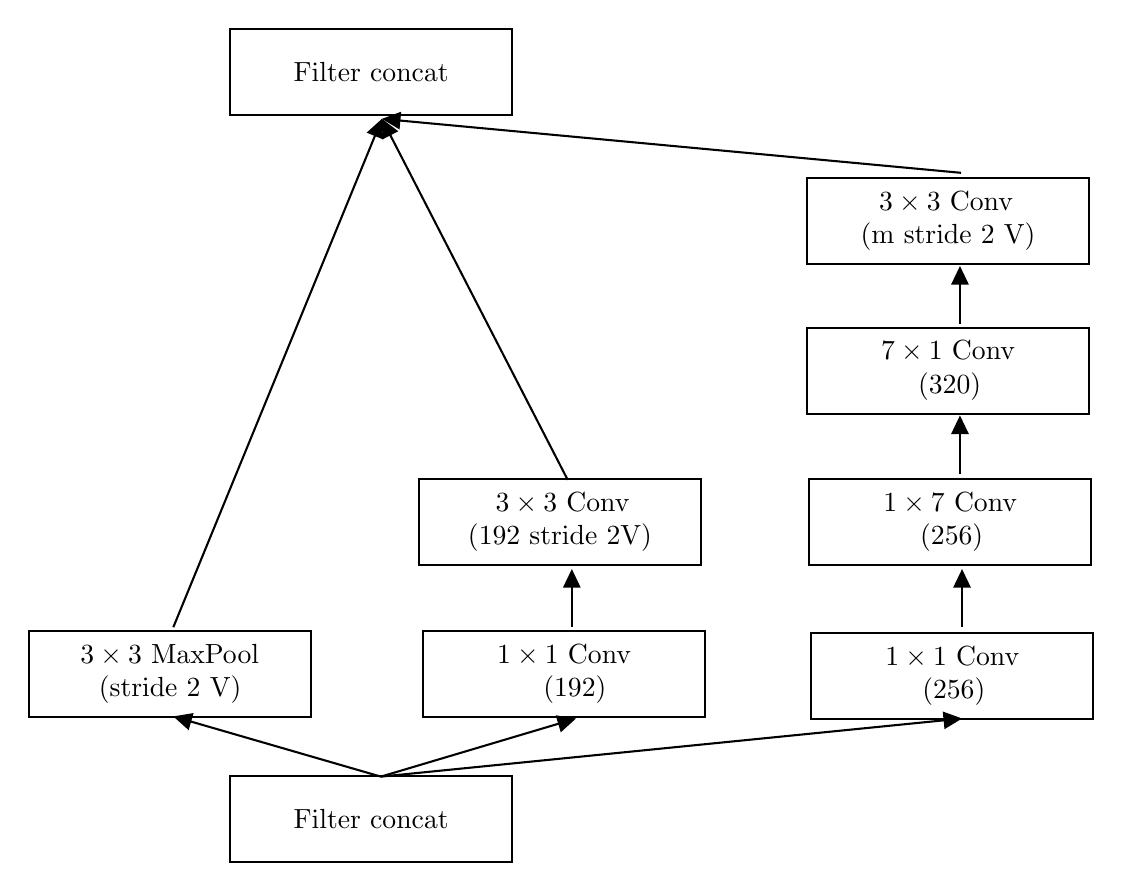
\begin{tikzpicture}[x=0.75pt,y=0.75pt,yscale=-1,xscale=1]
%uncomment if require: \path (0,470.3333282470703); %set diagram left start at 0, and has height of 470.3333282470703

%Flowchart: Process [id:dp24078826379297702] 
\draw   (528,418.9) -- (663.93,418.9) -- (663.93,460.33) -- (528,460.33) -- cycle ;
%Flowchart: Process [id:dp22165017848855517] 
\draw   (431,348.9) -- (566.93,348.9) -- (566.93,390.33) -- (431,390.33) -- cycle ;
%Flowchart: Process [id:dp6597264859137688] 
\draw   (621,348.9) -- (756.93,348.9) -- (756.93,390.33) -- (621,390.33) -- cycle ;
%Flowchart: Process [id:dp3799233367302206] 
\draw   (808,349.9) -- (943.93,349.9) -- (943.93,391.33) -- (808,391.33) -- cycle ;
%Straight Lines [id:da4490839848046586] 
\draw    (600.67,419.24) -- (502.59,390.8) ;
\draw [shift={(500.67,390.24)}, rotate = 376.16999999999996] [fill={rgb, 255:red, 0; green, 0; blue, 0 }  ][line width=0.75]  [draw opacity=0] (8.93,-4.29) -- (0,0) -- (8.93,4.29) -- cycle    ;

%Straight Lines [id:da38737183977033096] 
\draw    (600.67,419.24) -- (692.75,391.81) ;
\draw [shift={(694.67,391.24)}, rotate = 523.4100000000001] [fill={rgb, 255:red, 0; green, 0; blue, 0 }  ][line width=0.75]  [draw opacity=0] (8.93,-4.29) -- (0,0) -- (8.93,4.29) -- cycle    ;

%Straight Lines [id:da40057235552744497] 
\draw    (600.67,419.24) -- (878.68,391.44) ;
\draw [shift={(880.67,391.24)}, rotate = 534.29] [fill={rgb, 255:red, 0; green, 0; blue, 0 }  ][line width=0.75]  [draw opacity=0] (8.93,-4.29) -- (0,0) -- (8.93,4.29) -- cycle    ;

%Flowchart: Process [id:dp42511218119703864] 
\draw   (619,275.9) -- (754.93,275.9) -- (754.93,317.33) -- (619,317.33) -- cycle ;
%Flowchart: Process [id:dp6580432352234802] 
\draw   (807,275.9) -- (942.93,275.9) -- (942.93,317.33) -- (807,317.33) -- cycle ;
%Flowchart: Process [id:dp8669834254894924] 
\draw   (806,202.9) -- (941.93,202.9) -- (941.93,244.33) -- (806,244.33) -- cycle ;
%Straight Lines [id:da7396787751036953] 
\draw    (692.67,347.24) -- (692.67,321.24) ;
\draw [shift={(692.67,319.24)}, rotate = 450] [fill={rgb, 255:red, 0; green, 0; blue, 0 }  ][line width=0.75]  [draw opacity=0] (8.93,-4.29) -- (0,0) -- (8.93,4.29) -- cycle    ;

%Straight Lines [id:da2216611723462627] 
\draw    (880.67,347.24) -- (880.67,321.24) ;
\draw [shift={(880.67,319.24)}, rotate = 450] [fill={rgb, 255:red, 0; green, 0; blue, 0 }  ][line width=0.75]  [draw opacity=0] (8.93,-4.29) -- (0,0) -- (8.93,4.29) -- cycle    ;

%Straight Lines [id:da7609415385669374] 
\draw    (879.67,273.24) -- (879.67,247.24) ;
\draw [shift={(879.67,245.24)}, rotate = 450] [fill={rgb, 255:red, 0; green, 0; blue, 0 }  ][line width=0.75]  [draw opacity=0] (8.93,-4.29) -- (0,0) -- (8.93,4.29) -- cycle    ;

%Flowchart: Process [id:dp1491076780226832] 
\draw   (528,58.9) -- (663.93,58.9) -- (663.93,100.33) -- (528,100.33) -- cycle ;
%Straight Lines [id:da30781560796019103] 
\draw    (500.67,347.24) -- (600.41,104.18) ;
\draw [shift={(601.17,102.33)}, rotate = 472.31] [fill={rgb, 255:red, 0; green, 0; blue, 0 }  ][line width=0.75]  [draw opacity=0] (8.93,-4.29) -- (0,0) -- (8.93,4.29) -- cycle    ;

%Straight Lines [id:da24908463720618457] 
\draw    (690.67,276.24) -- (602.08,104.11) ;
\draw [shift={(601.17,102.33)}, rotate = 422.77] [fill={rgb, 255:red, 0; green, 0; blue, 0 }  ][line width=0.75]  [draw opacity=0] (8.93,-4.29) -- (0,0) -- (8.93,4.29) -- cycle    ;

%Flowchart: Process [id:dp01199680277761872] 
\draw   (806,130.9) -- (941.93,130.9) -- (941.93,172.33) -- (806,172.33) -- cycle ;
%Straight Lines [id:da3952124421996095] 
\draw    (879.67,201.24) -- (879.67,175.24) ;
\draw [shift={(879.67,173.24)}, rotate = 450] [fill={rgb, 255:red, 0; green, 0; blue, 0 }  ][line width=0.75]  [draw opacity=0] (8.93,-4.29) -- (0,0) -- (8.93,4.29) -- cycle    ;

%Straight Lines [id:da25220885973901197] 
\draw    (880.17,128.33) -- (603.16,102.52) ;
\draw [shift={(601.17,102.33)}, rotate = 365.32] [fill={rgb, 255:red, 0; green, 0; blue, 0 }  ][line width=0.75]  [draw opacity=0] (8.93,-4.29) -- (0,0) -- (8.93,4.29) -- cycle    ;


% Text Node
\draw (595.96,439.62) node  [align=left] {Filter concat};
% Text Node
\draw (498.96,369.62) node  [align=left] {$\displaystyle 3\times 3$ MaxPool\\ \ \ (stride $\displaystyle 2$ V)};
% Text Node
\draw (688.96,369.62) node  [align=left] {$\displaystyle 1\times 1$ Conv\\ \ \ \ \ \ ($\displaystyle 192$)};
% Text Node
\draw (875.96,370.62) node  [align=left] {$\displaystyle 1\times 1$ Conv\\ \ \ \ \ ($\displaystyle 256$)};
% Text Node
\draw (686.96,296.62) node  [align=left] {$\displaystyle \ \ \ 3\times 3$ Conv\\($\displaystyle 192$ stride $\displaystyle 2$V)};
% Text Node
\draw (874.96,296.62) node  [align=left] {$\displaystyle 1\times 7$ Conv\\ \ \ \ \ ($\displaystyle 256$)};
% Text Node
\draw (873.96,223.62) node  [align=left] {$\displaystyle 7\times 1$ Conv\\ \ \ \ \ ($\displaystyle 320$)};
% Text Node
\draw (595.96,79.62) node  [align=left] {Filter concat};
% Text Node
\draw (873.96,151.62) node  [align=left] {$\displaystyle \ \ 3\times 3$ Conv\\(m stride $\displaystyle 2$ V)};


\end{tikzpicture}}
   \caption{Reduction module (convolutions with "V" are valid, rest is same padded )}
   \label{fig:InceptionReduction}
\end{subfigure}

\caption{Special modules used by InceptionV4}

\end{figure}




Besides dropout InceptionV4 also benefits from the use of batch normalization during training.
%\begin{figure}[]
%\centering
%\resizebox{.45\linewidth}{!}{

\tikzset{every picture/.style={line width=0.75pt}} %set default line width to 0.75pt        

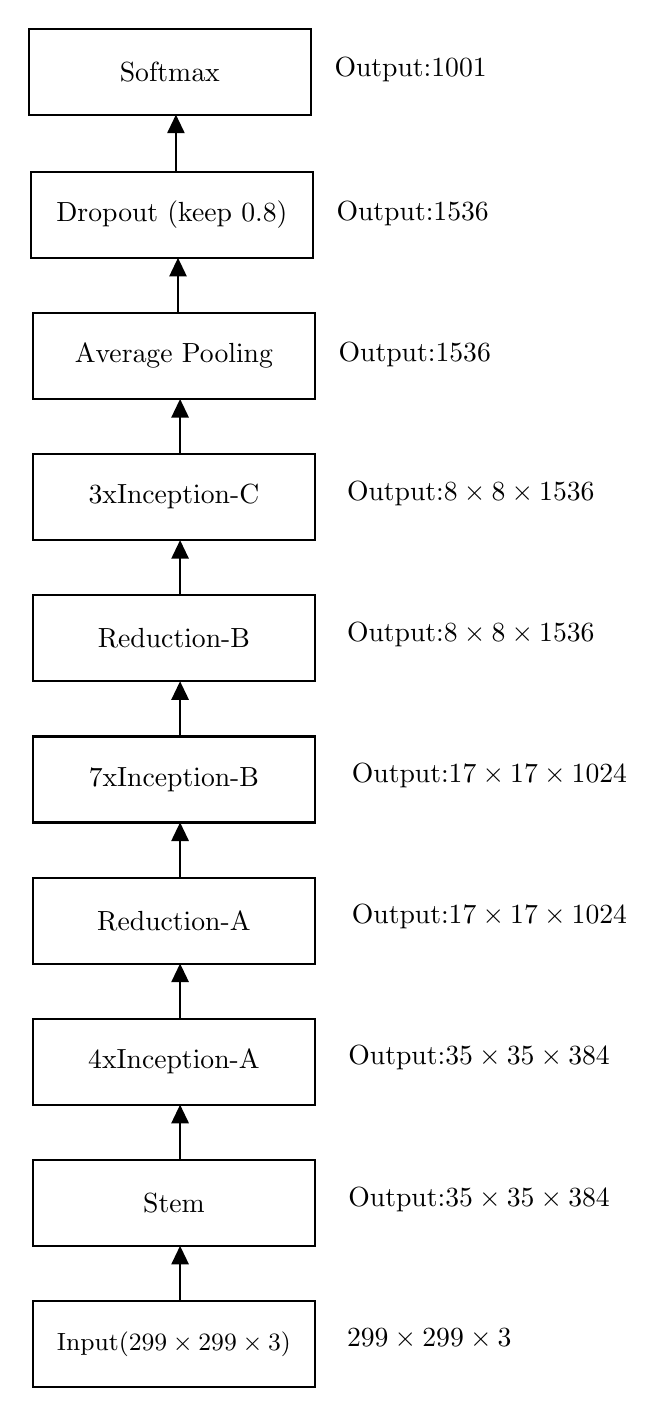
\begin{tikzpicture}[x=0.75pt,y=0.75pt,yscale=-1,xscale=1]
%uncomment if require: \path (0,742.7142868041992); %set diagram left start at 0, and has height of 742.7142868041992

%Flowchart: Process [id:dp9253173394290999] 
\draw   (98,621) -- (233.93,621) -- (233.93,662.43) -- (98,662.43) -- cycle ;
%Flowchart: Process [id:dp47578347996398307] 
\draw   (98,553) -- (233.93,553) -- (233.93,594.43) -- (98,594.43) -- cycle ;
%Straight Lines [id:da2925025767777827] 
\draw    (168.93,621.43) -- (168.93,596.43) ;
\draw [shift={(168.93,594.43)}, rotate = 450] [fill={rgb, 255:red, 0; green, 0; blue, 0 }  ][line width=0.75]  [draw opacity=0] (8.93,-4.29) -- (0,0) -- (8.93,4.29) -- cycle    ;

%Flowchart: Process [id:dp5382364848384393] 
\draw   (98,485) -- (233.93,485) -- (233.93,526.43) -- (98,526.43) -- cycle ;
%Straight Lines [id:da06940381159807729] 
\draw    (168.93,553.43) -- (168.93,528.43) ;
\draw [shift={(168.93,526.43)}, rotate = 450] [fill={rgb, 255:red, 0; green, 0; blue, 0 }  ][line width=0.75]  [draw opacity=0] (8.93,-4.29) -- (0,0) -- (8.93,4.29) -- cycle    ;

%Flowchart: Process [id:dp21301144435418706] 
\draw   (98,417) -- (233.93,417) -- (233.93,458.43) -- (98,458.43) -- cycle ;
%Straight Lines [id:da45627711718103714] 
\draw    (168.93,485.43) -- (168.93,460.43) ;
\draw [shift={(168.93,458.43)}, rotate = 450] [fill={rgb, 255:red, 0; green, 0; blue, 0 }  ][line width=0.75]  [draw opacity=0] (8.93,-4.29) -- (0,0) -- (8.93,4.29) -- cycle    ;

%Flowchart: Process [id:dp7231968775803179] 
\draw   (98,349) -- (233.93,349) -- (233.93,390.43) -- (98,390.43) -- cycle ;
%Straight Lines [id:da7165121439179447] 
\draw    (168.93,417.43) -- (168.93,392.43) ;
\draw [shift={(168.93,390.43)}, rotate = 450] [fill={rgb, 255:red, 0; green, 0; blue, 0 }  ][line width=0.75]  [draw opacity=0] (8.93,-4.29) -- (0,0) -- (8.93,4.29) -- cycle    ;

%Flowchart: Process [id:dp20620702942862734] 
\draw   (98,281) -- (233.93,281) -- (233.93,322.43) -- (98,322.43) -- cycle ;
%Straight Lines [id:da10564528480224444] 
\draw    (168.93,349.43) -- (168.93,324.43) ;
\draw [shift={(168.93,322.43)}, rotate = 450] [fill={rgb, 255:red, 0; green, 0; blue, 0 }  ][line width=0.75]  [draw opacity=0] (8.93,-4.29) -- (0,0) -- (8.93,4.29) -- cycle    ;

%Flowchart: Process [id:dp6409642010028676] 
\draw   (98,213) -- (233.93,213) -- (233.93,254.43) -- (98,254.43) -- cycle ;
%Straight Lines [id:da583110185704452] 
\draw    (168.93,281.43) -- (168.93,256.43) ;
\draw [shift={(168.93,254.43)}, rotate = 450] [fill={rgb, 255:red, 0; green, 0; blue, 0 }  ][line width=0.75]  [draw opacity=0] (8.93,-4.29) -- (0,0) -- (8.93,4.29) -- cycle    ;

%Flowchart: Process [id:dp747253235525678] 
\draw   (98,145) -- (233.93,145) -- (233.93,186.43) -- (98,186.43) -- cycle ;
%Straight Lines [id:da9482962038382927] 
\draw    (168.93,213.43) -- (168.93,188.43) ;
\draw [shift={(168.93,186.43)}, rotate = 450] [fill={rgb, 255:red, 0; green, 0; blue, 0 }  ][line width=0.75]  [draw opacity=0] (8.93,-4.29) -- (0,0) -- (8.93,4.29) -- cycle    ;

%Flowchart: Process [id:dp47103409298757426] 
\draw   (97,77) -- (232.93,77) -- (232.93,118.43) -- (97,118.43) -- cycle ;
%Straight Lines [id:da30249651940608824] 
\draw    (167.93,145.43) -- (167.93,120.43) ;
\draw [shift={(167.93,118.43)}, rotate = 450] [fill={rgb, 255:red, 0; green, 0; blue, 0 }  ][line width=0.75]  [draw opacity=0] (8.93,-4.29) -- (0,0) -- (8.93,4.29) -- cycle    ;

%Flowchart: Process [id:dp5661311837160838] 
\draw   (96,8) -- (231.93,8) -- (231.93,49.43) -- (96,49.43) -- cycle ;
%Straight Lines [id:da5142446239913938] 
\draw    (166.93,76.43) -- (166.93,51.43) ;
\draw [shift={(166.93,49.43)}, rotate = 450] [fill={rgb, 255:red, 0; green, 0; blue, 0 }  ][line width=0.75]  [draw opacity=0] (8.93,-4.29) -- (0,0) -- (8.93,4.29) -- cycle    ;


% Text Node
\draw (165.96,641.71) node  [align=left] {{\small Input($\displaystyle 299\times 299\times 3$)}};
% Text Node
\draw (165.96,573.71) node  [align=left] {Stem};
% Text Node
\draw (289,639) node  [align=left] {$\displaystyle 299\times 299\times 3$};
% Text Node
\draw (313,572) node  [align=left] {Output:$\displaystyle 35\times 35\times 384$};
% Text Node
\draw (165.96,505.71) node  [align=left] {4xInception-A};
% Text Node
\draw (313,504) node  [align=left] {Output:$\displaystyle 35\times 35\times 384$};
% Text Node
\draw (165.96,437.71) node  [align=left] {Reduction-A};
% Text Node
\draw (318,436) node  [align=left] {Output:$\displaystyle 17\times 17\times 1024$};
% Text Node
\draw (165.96,369.71) node  [align=left] {7xInception-B};
% Text Node
\draw (318,368) node  [align=left] {Output:$\displaystyle 17\times 17\times 1024$};
% Text Node
\draw (165.96,301.71) node  [align=left] {Reduction-B};
% Text Node
\draw (309,300) node  [align=left] {Output:$\displaystyle 8\times 8\times 1536$};
% Text Node
\draw (165.96,233.71) node  [align=left] {3xInception-C};
% Text Node
\draw (309,232) node  [align=left] {Output:$\displaystyle 8\times 8\times 1536$};
% Text Node
\draw (165.96,165.71) node  [align=left] {Average Pooling};
% Text Node
\draw (282,165) node  [align=left] {Output:$\displaystyle 1536$};
% Text Node
\draw (164.96,97.71) node  [align=left] {Dropout (keep $\displaystyle 0.8$)};
% Text Node
\draw (281,97) node  [align=left] {Output:$\displaystyle 1536$};
% Text Node
\draw (163.96,28.71) node  [align=left] {Softmax};
% Text Node
\draw (280,28) node  [align=left] {Output:$\displaystyle 1001$};


\end{tikzpicture}}
%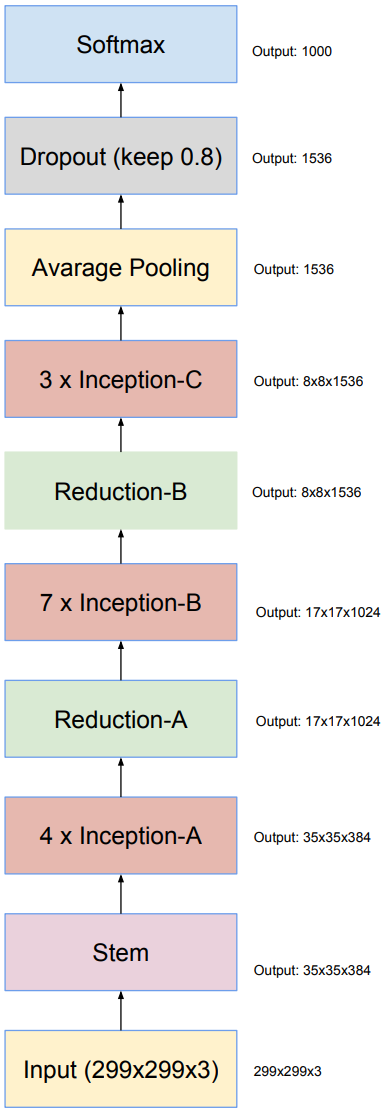
\includegraphics[angle=90,width=0.94\textwidth]{./Bilder/inceptionV4_architecture.png}
%\caption{InceptionV4 architecture \cite{InceptionV4}}
%\label{fig:inceptionv4}
%\end{figure}

\begin{figure}[!htb]
\centering
\begin{subfigure}[t]{0.47\textwidth}
   \resizebox{.99\linewidth}{!}{

\tikzset{every picture/.style={line width=0.75pt}} %set default line width to 0.75pt        

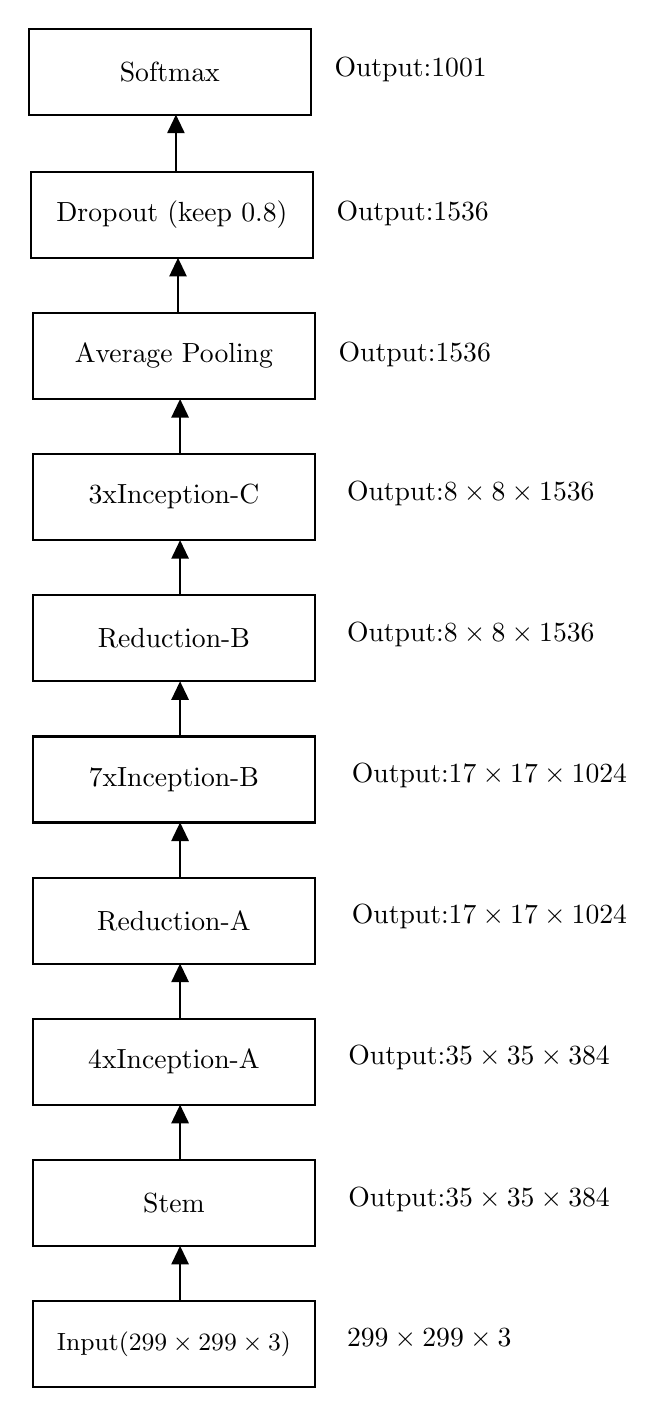
\begin{tikzpicture}[x=0.75pt,y=0.75pt,yscale=-1,xscale=1]
%uncomment if require: \path (0,742.7142868041992); %set diagram left start at 0, and has height of 742.7142868041992

%Flowchart: Process [id:dp9253173394290999] 
\draw   (98,621) -- (233.93,621) -- (233.93,662.43) -- (98,662.43) -- cycle ;
%Flowchart: Process [id:dp47578347996398307] 
\draw   (98,553) -- (233.93,553) -- (233.93,594.43) -- (98,594.43) -- cycle ;
%Straight Lines [id:da2925025767777827] 
\draw    (168.93,621.43) -- (168.93,596.43) ;
\draw [shift={(168.93,594.43)}, rotate = 450] [fill={rgb, 255:red, 0; green, 0; blue, 0 }  ][line width=0.75]  [draw opacity=0] (8.93,-4.29) -- (0,0) -- (8.93,4.29) -- cycle    ;

%Flowchart: Process [id:dp5382364848384393] 
\draw   (98,485) -- (233.93,485) -- (233.93,526.43) -- (98,526.43) -- cycle ;
%Straight Lines [id:da06940381159807729] 
\draw    (168.93,553.43) -- (168.93,528.43) ;
\draw [shift={(168.93,526.43)}, rotate = 450] [fill={rgb, 255:red, 0; green, 0; blue, 0 }  ][line width=0.75]  [draw opacity=0] (8.93,-4.29) -- (0,0) -- (8.93,4.29) -- cycle    ;

%Flowchart: Process [id:dp21301144435418706] 
\draw   (98,417) -- (233.93,417) -- (233.93,458.43) -- (98,458.43) -- cycle ;
%Straight Lines [id:da45627711718103714] 
\draw    (168.93,485.43) -- (168.93,460.43) ;
\draw [shift={(168.93,458.43)}, rotate = 450] [fill={rgb, 255:red, 0; green, 0; blue, 0 }  ][line width=0.75]  [draw opacity=0] (8.93,-4.29) -- (0,0) -- (8.93,4.29) -- cycle    ;

%Flowchart: Process [id:dp7231968775803179] 
\draw   (98,349) -- (233.93,349) -- (233.93,390.43) -- (98,390.43) -- cycle ;
%Straight Lines [id:da7165121439179447] 
\draw    (168.93,417.43) -- (168.93,392.43) ;
\draw [shift={(168.93,390.43)}, rotate = 450] [fill={rgb, 255:red, 0; green, 0; blue, 0 }  ][line width=0.75]  [draw opacity=0] (8.93,-4.29) -- (0,0) -- (8.93,4.29) -- cycle    ;

%Flowchart: Process [id:dp20620702942862734] 
\draw   (98,281) -- (233.93,281) -- (233.93,322.43) -- (98,322.43) -- cycle ;
%Straight Lines [id:da10564528480224444] 
\draw    (168.93,349.43) -- (168.93,324.43) ;
\draw [shift={(168.93,322.43)}, rotate = 450] [fill={rgb, 255:red, 0; green, 0; blue, 0 }  ][line width=0.75]  [draw opacity=0] (8.93,-4.29) -- (0,0) -- (8.93,4.29) -- cycle    ;

%Flowchart: Process [id:dp6409642010028676] 
\draw   (98,213) -- (233.93,213) -- (233.93,254.43) -- (98,254.43) -- cycle ;
%Straight Lines [id:da583110185704452] 
\draw    (168.93,281.43) -- (168.93,256.43) ;
\draw [shift={(168.93,254.43)}, rotate = 450] [fill={rgb, 255:red, 0; green, 0; blue, 0 }  ][line width=0.75]  [draw opacity=0] (8.93,-4.29) -- (0,0) -- (8.93,4.29) -- cycle    ;

%Flowchart: Process [id:dp747253235525678] 
\draw   (98,145) -- (233.93,145) -- (233.93,186.43) -- (98,186.43) -- cycle ;
%Straight Lines [id:da9482962038382927] 
\draw    (168.93,213.43) -- (168.93,188.43) ;
\draw [shift={(168.93,186.43)}, rotate = 450] [fill={rgb, 255:red, 0; green, 0; blue, 0 }  ][line width=0.75]  [draw opacity=0] (8.93,-4.29) -- (0,0) -- (8.93,4.29) -- cycle    ;

%Flowchart: Process [id:dp47103409298757426] 
\draw   (97,77) -- (232.93,77) -- (232.93,118.43) -- (97,118.43) -- cycle ;
%Straight Lines [id:da30249651940608824] 
\draw    (167.93,145.43) -- (167.93,120.43) ;
\draw [shift={(167.93,118.43)}, rotate = 450] [fill={rgb, 255:red, 0; green, 0; blue, 0 }  ][line width=0.75]  [draw opacity=0] (8.93,-4.29) -- (0,0) -- (8.93,4.29) -- cycle    ;

%Flowchart: Process [id:dp5661311837160838] 
\draw   (96,8) -- (231.93,8) -- (231.93,49.43) -- (96,49.43) -- cycle ;
%Straight Lines [id:da5142446239913938] 
\draw    (166.93,76.43) -- (166.93,51.43) ;
\draw [shift={(166.93,49.43)}, rotate = 450] [fill={rgb, 255:red, 0; green, 0; blue, 0 }  ][line width=0.75]  [draw opacity=0] (8.93,-4.29) -- (0,0) -- (8.93,4.29) -- cycle    ;


% Text Node
\draw (165.96,641.71) node  [align=left] {{\small Input($\displaystyle 299\times 299\times 3$)}};
% Text Node
\draw (165.96,573.71) node  [align=left] {Stem};
% Text Node
\draw (289,639) node  [align=left] {$\displaystyle 299\times 299\times 3$};
% Text Node
\draw (313,572) node  [align=left] {Output:$\displaystyle 35\times 35\times 384$};
% Text Node
\draw (165.96,505.71) node  [align=left] {4xInception-A};
% Text Node
\draw (313,504) node  [align=left] {Output:$\displaystyle 35\times 35\times 384$};
% Text Node
\draw (165.96,437.71) node  [align=left] {Reduction-A};
% Text Node
\draw (318,436) node  [align=left] {Output:$\displaystyle 17\times 17\times 1024$};
% Text Node
\draw (165.96,369.71) node  [align=left] {7xInception-B};
% Text Node
\draw (318,368) node  [align=left] {Output:$\displaystyle 17\times 17\times 1024$};
% Text Node
\draw (165.96,301.71) node  [align=left] {Reduction-B};
% Text Node
\draw (309,300) node  [align=left] {Output:$\displaystyle 8\times 8\times 1536$};
% Text Node
\draw (165.96,233.71) node  [align=left] {3xInception-C};
% Text Node
\draw (309,232) node  [align=left] {Output:$\displaystyle 8\times 8\times 1536$};
% Text Node
\draw (165.96,165.71) node  [align=left] {Average Pooling};
% Text Node
\draw (282,165) node  [align=left] {Output:$\displaystyle 1536$};
% Text Node
\draw (164.96,97.71) node  [align=left] {Dropout (keep $\displaystyle 0.8$)};
% Text Node
\draw (281,97) node  [align=left] {Output:$\displaystyle 1536$};
% Text Node
\draw (163.96,28.71) node  [align=left] {Softmax};
% Text Node
\draw (280,28) node  [align=left] {Output:$\displaystyle 1001$};


\end{tikzpicture}}
   \caption{InceptionV4 architecture \cite{InceptionV4}}
   \label{fig:inceptionv4Archi} 
\end{subfigure}%
\begin{subfigure}[t]{0.47\textwidth}
   %%Verify the architectures again
   \resizebox{.99\linewidth}{!}{

\tikzset{every picture/.style={line width=0.75pt}} %set default line width to 0.75pt        

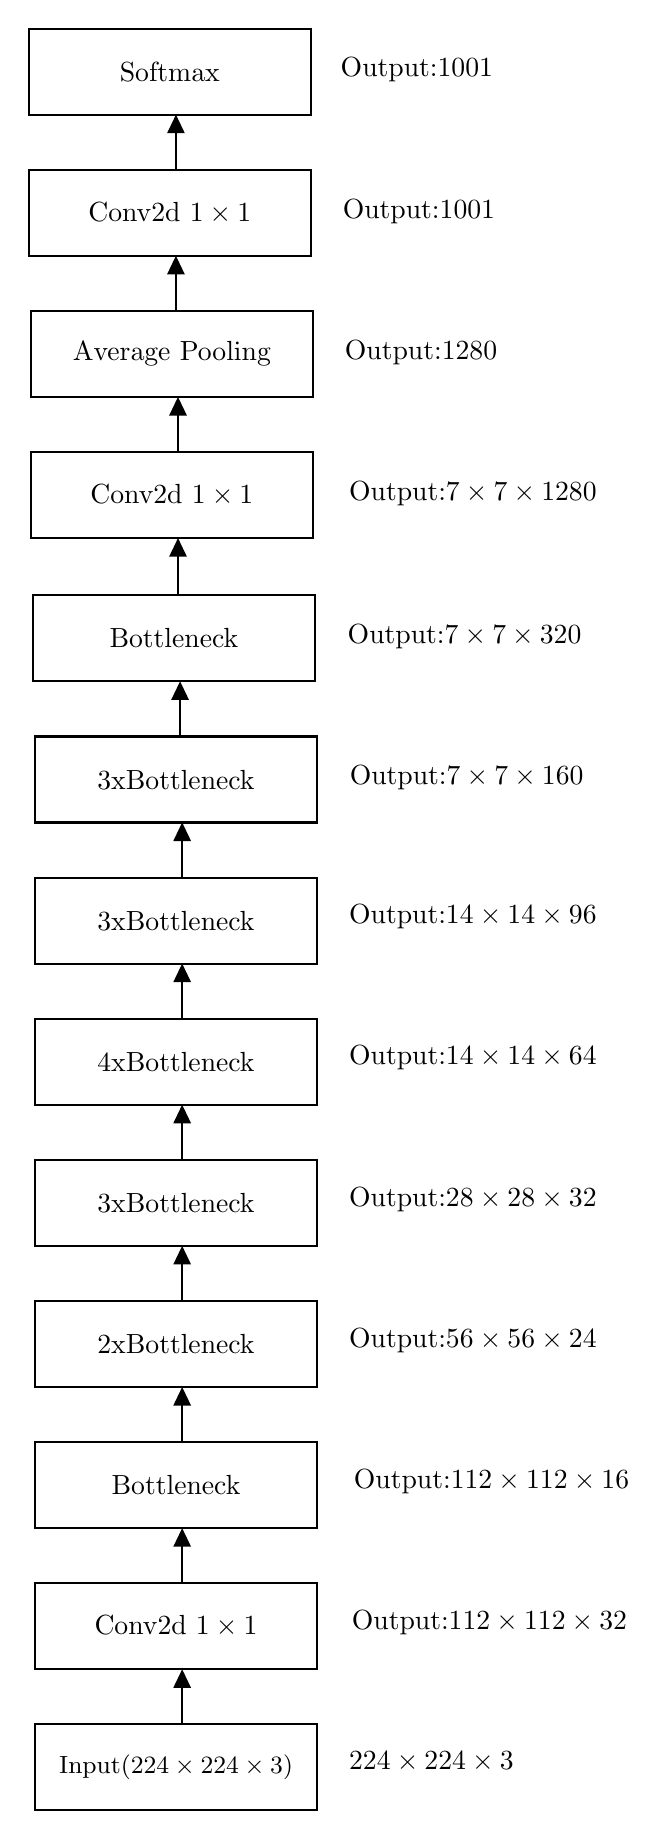
\begin{tikzpicture}[x=0.75pt,y=0.75pt,yscale=-1,xscale=1]
%uncomment if require: \path (0,948.6666870117188); %set diagram left start at 0, and has height of 948.6666870117188

%Flowchart: Process [id:dp9253173394290999] 
\draw   (98,897) -- (233.93,897) -- (233.93,938.43) -- (98,938.43) -- cycle ;
%Flowchart: Process [id:dp47578347996398307] 
\draw   (98,829) -- (233.93,829) -- (233.93,870.43) -- (98,870.43) -- cycle ;
%Straight Lines [id:da2925025767777827] 
\draw    (168.93,897.43) -- (168.93,872.43) ;
\draw [shift={(168.93,870.43)}, rotate = 450] [fill={rgb, 255:red, 0; green, 0; blue, 0 }  ][line width=0.75]  [draw opacity=0] (8.93,-4.29) -- (0,0) -- (8.93,4.29) -- cycle    ;

%Flowchart: Process [id:dp5382364848384393] 
\draw   (98,761) -- (233.93,761) -- (233.93,802.43) -- (98,802.43) -- cycle ;
%Straight Lines [id:da06940381159807729] 
\draw    (168.93,829.43) -- (168.93,804.43) ;
\draw [shift={(168.93,802.43)}, rotate = 450] [fill={rgb, 255:red, 0; green, 0; blue, 0 }  ][line width=0.75]  [draw opacity=0] (8.93,-4.29) -- (0,0) -- (8.93,4.29) -- cycle    ;

%Flowchart: Process [id:dp21301144435418706] 
\draw   (98,693) -- (233.93,693) -- (233.93,734.43) -- (98,734.43) -- cycle ;
%Straight Lines [id:da45627711718103714] 
\draw    (168.93,761.43) -- (168.93,736.43) ;
\draw [shift={(168.93,734.43)}, rotate = 450] [fill={rgb, 255:red, 0; green, 0; blue, 0 }  ][line width=0.75]  [draw opacity=0] (8.93,-4.29) -- (0,0) -- (8.93,4.29) -- cycle    ;

%Flowchart: Process [id:dp7231968775803179] 
\draw   (98,625) -- (233.93,625) -- (233.93,666.43) -- (98,666.43) -- cycle ;
%Straight Lines [id:da7165121439179447] 
\draw    (168.93,693.43) -- (168.93,668.43) ;
\draw [shift={(168.93,666.43)}, rotate = 450] [fill={rgb, 255:red, 0; green, 0; blue, 0 }  ][line width=0.75]  [draw opacity=0] (8.93,-4.29) -- (0,0) -- (8.93,4.29) -- cycle    ;

%Flowchart: Process [id:dp20620702942862734] 
\draw   (98,557) -- (233.93,557) -- (233.93,598.43) -- (98,598.43) -- cycle ;
%Straight Lines [id:da10564528480224444] 
\draw    (168.93,625.43) -- (168.93,600.43) ;
\draw [shift={(168.93,598.43)}, rotate = 450] [fill={rgb, 255:red, 0; green, 0; blue, 0 }  ][line width=0.75]  [draw opacity=0] (8.93,-4.29) -- (0,0) -- (8.93,4.29) -- cycle    ;

%Flowchart: Process [id:dp6409642010028676] 
\draw   (98,489) -- (233.93,489) -- (233.93,530.43) -- (98,530.43) -- cycle ;
%Straight Lines [id:da583110185704452] 
\draw    (168.93,557.43) -- (168.93,532.43) ;
\draw [shift={(168.93,530.43)}, rotate = 450] [fill={rgb, 255:red, 0; green, 0; blue, 0 }  ][line width=0.75]  [draw opacity=0] (8.93,-4.29) -- (0,0) -- (8.93,4.29) -- cycle    ;

%Flowchart: Process [id:dp747253235525678] 
\draw   (98,421) -- (233.93,421) -- (233.93,462.43) -- (98,462.43) -- cycle ;
%Straight Lines [id:da9482962038382927] 
\draw    (168.93,489.43) -- (168.93,464.43) ;
\draw [shift={(168.93,462.43)}, rotate = 450] [fill={rgb, 255:red, 0; green, 0; blue, 0 }  ][line width=0.75]  [draw opacity=0] (8.93,-4.29) -- (0,0) -- (8.93,4.29) -- cycle    ;

%Flowchart: Process [id:dp47103409298757426] 
\draw   (97,353) -- (232.93,353) -- (232.93,394.43) -- (97,394.43) -- cycle ;
%Straight Lines [id:da30249651940608824] 
\draw    (167.93,421.43) -- (167.93,396.43) ;
\draw [shift={(167.93,394.43)}, rotate = 450] [fill={rgb, 255:red, 0; green, 0; blue, 0 }  ][line width=0.75]  [draw opacity=0] (8.93,-4.29) -- (0,0) -- (8.93,4.29) -- cycle    ;

%Flowchart: Process [id:dp5661311837160838] 
\draw   (96,284) -- (231.93,284) -- (231.93,325.43) -- (96,325.43) -- cycle ;
%Straight Lines [id:da5142446239913938] 
\draw    (166.93,352.43) -- (166.93,327.43) ;
\draw [shift={(166.93,325.43)}, rotate = 450] [fill={rgb, 255:red, 0; green, 0; blue, 0 }  ][line width=0.75]  [draw opacity=0] (8.93,-4.29) -- (0,0) -- (8.93,4.29) -- cycle    ;

%Flowchart: Process [id:dp8648151912409288] 
\draw   (96,216) -- (231.93,216) -- (231.93,257.43) -- (96,257.43) -- cycle ;
%Straight Lines [id:da21788225541174455] 
\draw    (166.93,284.43) -- (166.93,259.43) ;
\draw [shift={(166.93,257.43)}, rotate = 450] [fill={rgb, 255:red, 0; green, 0; blue, 0 }  ][line width=0.75]  [draw opacity=0] (8.93,-4.29) -- (0,0) -- (8.93,4.29) -- cycle    ;

%Flowchart: Process [id:dp5915277931570215] 
\draw   (95,148) -- (230.93,148) -- (230.93,189.43) -- (95,189.43) -- cycle ;
%Straight Lines [id:da2169186042376452] 
\draw    (165.93,216.43) -- (165.93,191.43) ;
\draw [shift={(165.93,189.43)}, rotate = 450] [fill={rgb, 255:red, 0; green, 0; blue, 0 }  ][line width=0.75]  [draw opacity=0] (8.93,-4.29) -- (0,0) -- (8.93,4.29) -- cycle    ;

%Flowchart: Process [id:dp09241683513730559] 
\draw   (95,80) -- (230.93,80) -- (230.93,121.43) -- (95,121.43) -- cycle ;
%Straight Lines [id:da3985231842573671] 
\draw    (165.93,148.43) -- (165.93,123.43) ;
\draw [shift={(165.93,121.43)}, rotate = 450] [fill={rgb, 255:red, 0; green, 0; blue, 0 }  ][line width=0.75]  [draw opacity=0] (8.93,-4.29) -- (0,0) -- (8.93,4.29) -- cycle    ;


% Text Node
\draw (165.96,917.71) node  [align=left] {{\small Input($\displaystyle 224\times 224\times 3$)}};
% Text Node
\draw (165.96,849.71) node  [align=left] {Conv2d $\displaystyle 1\times 1$};
% Text Node
\draw (289,915) node  [align=left] {$\displaystyle 224\times 224\times 3$};
% Text Node
\draw (317,848) node  [align=left] {Output:$\displaystyle 112\times 112\times 32$};
% Text Node
\draw (165.96,781.71) node  [align=left] {Bottleneck};
% Text Node
\draw (318,780) node  [align=left] {Output:$\displaystyle 112\times 112\times 16$};
% Text Node
\draw (165.96,713.71) node  [align=left] {2xBottleneck};
% Text Node
\draw (309,712) node  [align=left] {Output:$\displaystyle 56\times 56\times 24$};
% Text Node
\draw (165.96,645.71) node  [align=left] {3xBottleneck};
% Text Node
\draw (309,644) node  [align=left] {Output:$\displaystyle 28\times 28\times 32$};
% Text Node
\draw (165.96,577.71) node  [align=left] {4xBottleneck};
% Text Node
\draw (309,576) node  [align=left] {Output:$\displaystyle 14\times 14\times 64$};
% Text Node
\draw (165.96,509.71) node  [align=left] {3xBottleneck};
% Text Node
\draw (309,508) node  [align=left] {Output:$\displaystyle 14\times 14\times 96$};
% Text Node
\draw (165.96,441.71) node  [align=left] {3xBottleneck};
% Text Node
\draw (306,441) node  [align=left] {Output:$\displaystyle 7\times 7\times 160$};
% Text Node
\draw (164.96,373.71) node  [align=left] {Bottleneck};
% Text Node
\draw (305,373) node  [align=left] {Output:$\displaystyle 7\times 7\times 320$};
% Text Node
\draw (163.96,304.71) node  [align=left] {Conv2d $\displaystyle 1\times 1$};
% Text Node
\draw (309,304) node  [align=left] {Output:$\displaystyle 7\times 7\times 1280$};
% Text Node
\draw (163.96,236.71) node  [align=left] {Average Pooling};
% Text Node
\draw (284,236) node  [align=left] {Output:$\displaystyle 1280$};
% Text Node
\draw (162.96,168.71) node  [align=left] {Conv2d $\displaystyle 1\times 1$};
% Text Node
\draw (283,168) node  [align=left] {Output:$\displaystyle 1001$};
% Text Node
\draw (162.96,100.71) node  [align=left] {Softmax};
% Text Node
\draw (282,100) node  [align=left] {Output:$\displaystyle 1001$};


\end{tikzpicture}}
   \caption{MobileNetV2 architecture \cite{DBLP:journals/corr/abs-1801-04381}}
   \label{fig:MobileNetArchi}
\end{subfigure}

\caption{Architectures of InceptionV4 and MobileNetV2}
%%NO DROPOUT AT INFERENCE
\end{figure}



\subsection{Android Benchmark Application}
\label{chap:androidApp}
To conduct the experiments for both edge and cloud inference we developed and implemented an Android benchmark application using Kotlin.
This application implements all function needed to preprocess real workload images and perform the inference on either the Android device itself or sent the image to a cloud-backend.
For both preprocessing and inference the application logs metrics such as inference latency, time of the experiments etc. and stores them to a \emph{CSV} file, which then can be used to evaluation purposes.

Both edge and cloud inference implementations are based on the example implementations in the respective GitHub repositories to ensure optimal performance. 


\begin{figure}[htb]
\centering
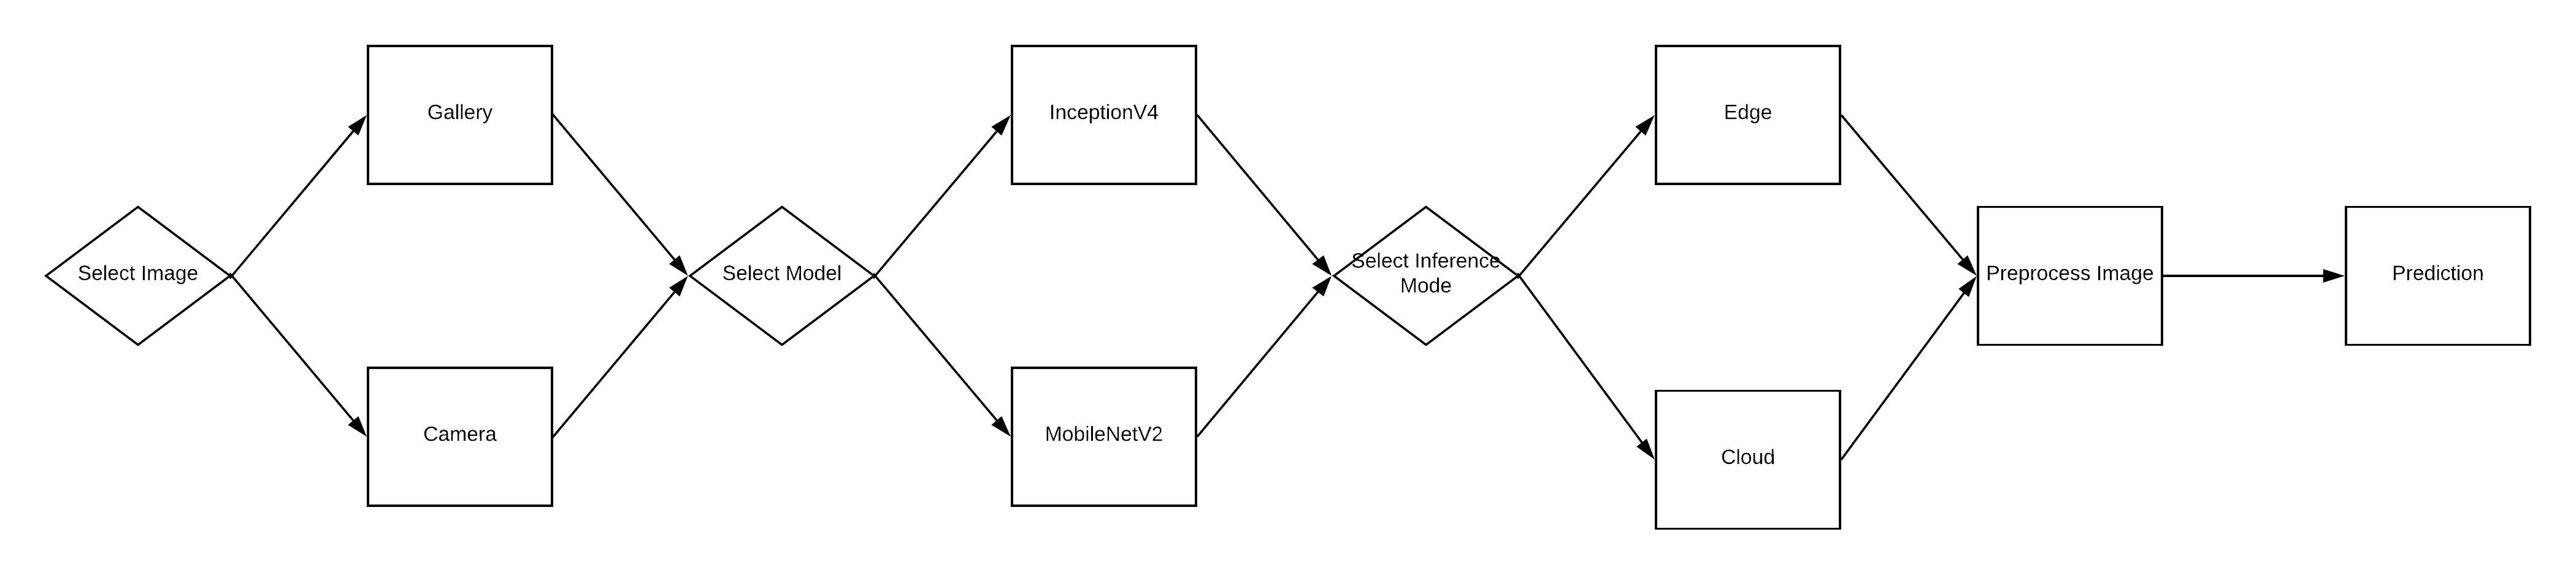
\includegraphics[width=0.97\textwidth]{./Bilder/FlowChart_App.png}
\caption{Flowchart of the Benchmark Application showing the whole inference process of selecting an image until getting a prediction}
\label{fig:app}
\end{figure}
In figure \ref{fig:app} the work-flow to perform the inference is seen. First, a image needs to be selected. Afterwards the image classification model needs to be chosen. Now the user selects whether the inference should be performed on the cloud-backend or directly on the edge device, in this case a Android phone. In the case of edge inference it needs to be decided if the NNAPI should be used by TensorFlow Lite. For cloud inference the preprocessing mode needs to be selected (edge/cloud). Now the preprocessing operations can be performed based on the previous selected options (Even for the case of cloud inference with cloud preprocessing some preprocessing needs to be done on the edge beforehand like building a \emph{PredictRequest} containing the request for the cloud-backend). Now, that the input is preprocessed, the actual inference is performed as a last step, resulting in a prediction. For both preprocessing and inference the measurements mentioned in section \ref{chap:insta_measurements} are logged.

\begin{figure}[htb]
\centering
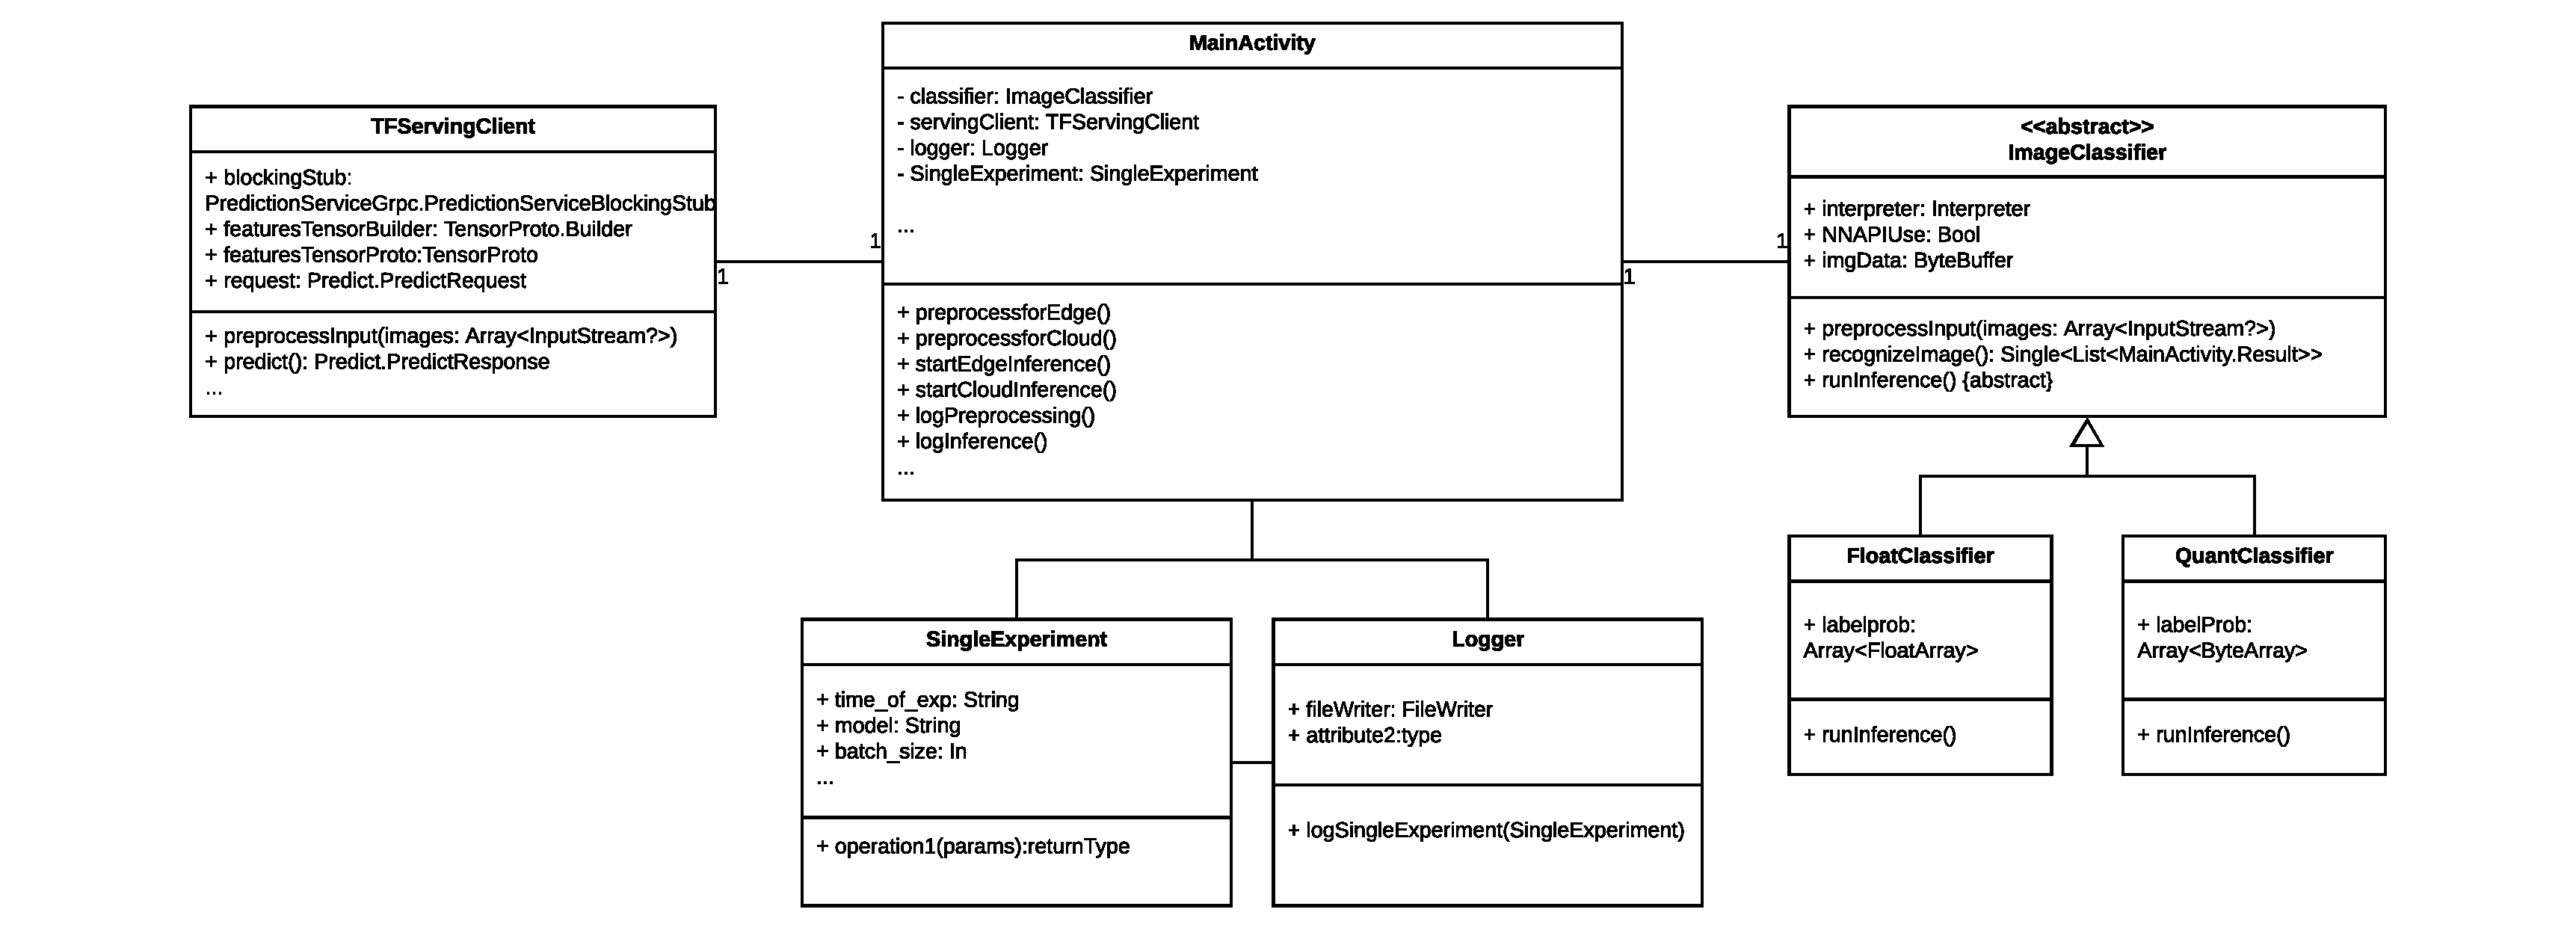
\includegraphics[width=0.99\textwidth]{./Bilder/UML.pdf}
\caption{UML class diagram of the benchmark application}
\label{fig:UML}
\end{figure}
Figure \ref{fig:UML} depicts an UML class diagram of the application featuring the most important classes, functions and variables. 
The main class is called \emph{MainActivity} and implements all of the graphical aspects. 
The \emph{MainActivity} handles requests for both cloud and edge inference by delegating the requests to instances of the classes \emph{TFServingClient} and \emph{ImageClassifier}, respectively. Both of these classes also take care of the preprocessing steps.
The abstract class \emph{ImageClassifier} has two subclasses \emph{FloatClassifier} and \emph{QuantClassifier}. The first class runs the inference for floating point models and the second for quantized models.
This separation is needed since these different model types require different input and output types.

The \emph{MainActivity} writes the collected measurements and the parameter configurations of an experiment to a instance of \emph{SingleExperiment}. After the experiment is completed \emph{MainActivity} tells a \emph{Logger} instance to save the contents of the \emph{SingleExperiment} object. The Logger then saves all collected data to a \emph{CSV} file.

\subsubsection{Preprocessing}
%%mention png
For the case of image classification, the images need to have the correct size ($224\times224$ for MobilenetV2 and $299\times299$ for InceptionV4) and the RGB values need to be normalized to the interval $[-1,1]$. After preprocessing the image has been transformed into the shape $224\times224\times3$ with all values between $[-1,1]$, where the the first two dimensions represent the image height and width, while the last dimension represent the number of channels (3 since the images are RGB)
\begin{figure}[H]
\centering


\tikzset{every picture/.style={line width=0.75pt}} %set default line width to 0.75pt        

\begin{tikzpicture}[x=0.75pt,y=0.75pt,yscale=-1,xscale=1]
%uncomment if require: \path (0,484.3333282470703); %set diagram left start at 0, and has height of 484.3333282470703

%Shape: Square [id:dp1081653036325061] 
\draw  [fill={rgb, 255:red, 0; green, 0; blue, 255 }  ,fill opacity=1 ] (217.67,92) -- (317,92) -- (317,191.33) -- (217.67,191.33) -- cycle ;
%Shape: Square [id:dp8785233930816818] 
\draw  [fill={rgb, 255:red, 0; green, 255; blue, 0 }  ,fill opacity=1 ] (207.67,100) -- (307,100) -- (307,199.33) -- (207.67,199.33) -- cycle ;
%Image [id:dp7451570314710638] 
\draw (67,158.49) node  {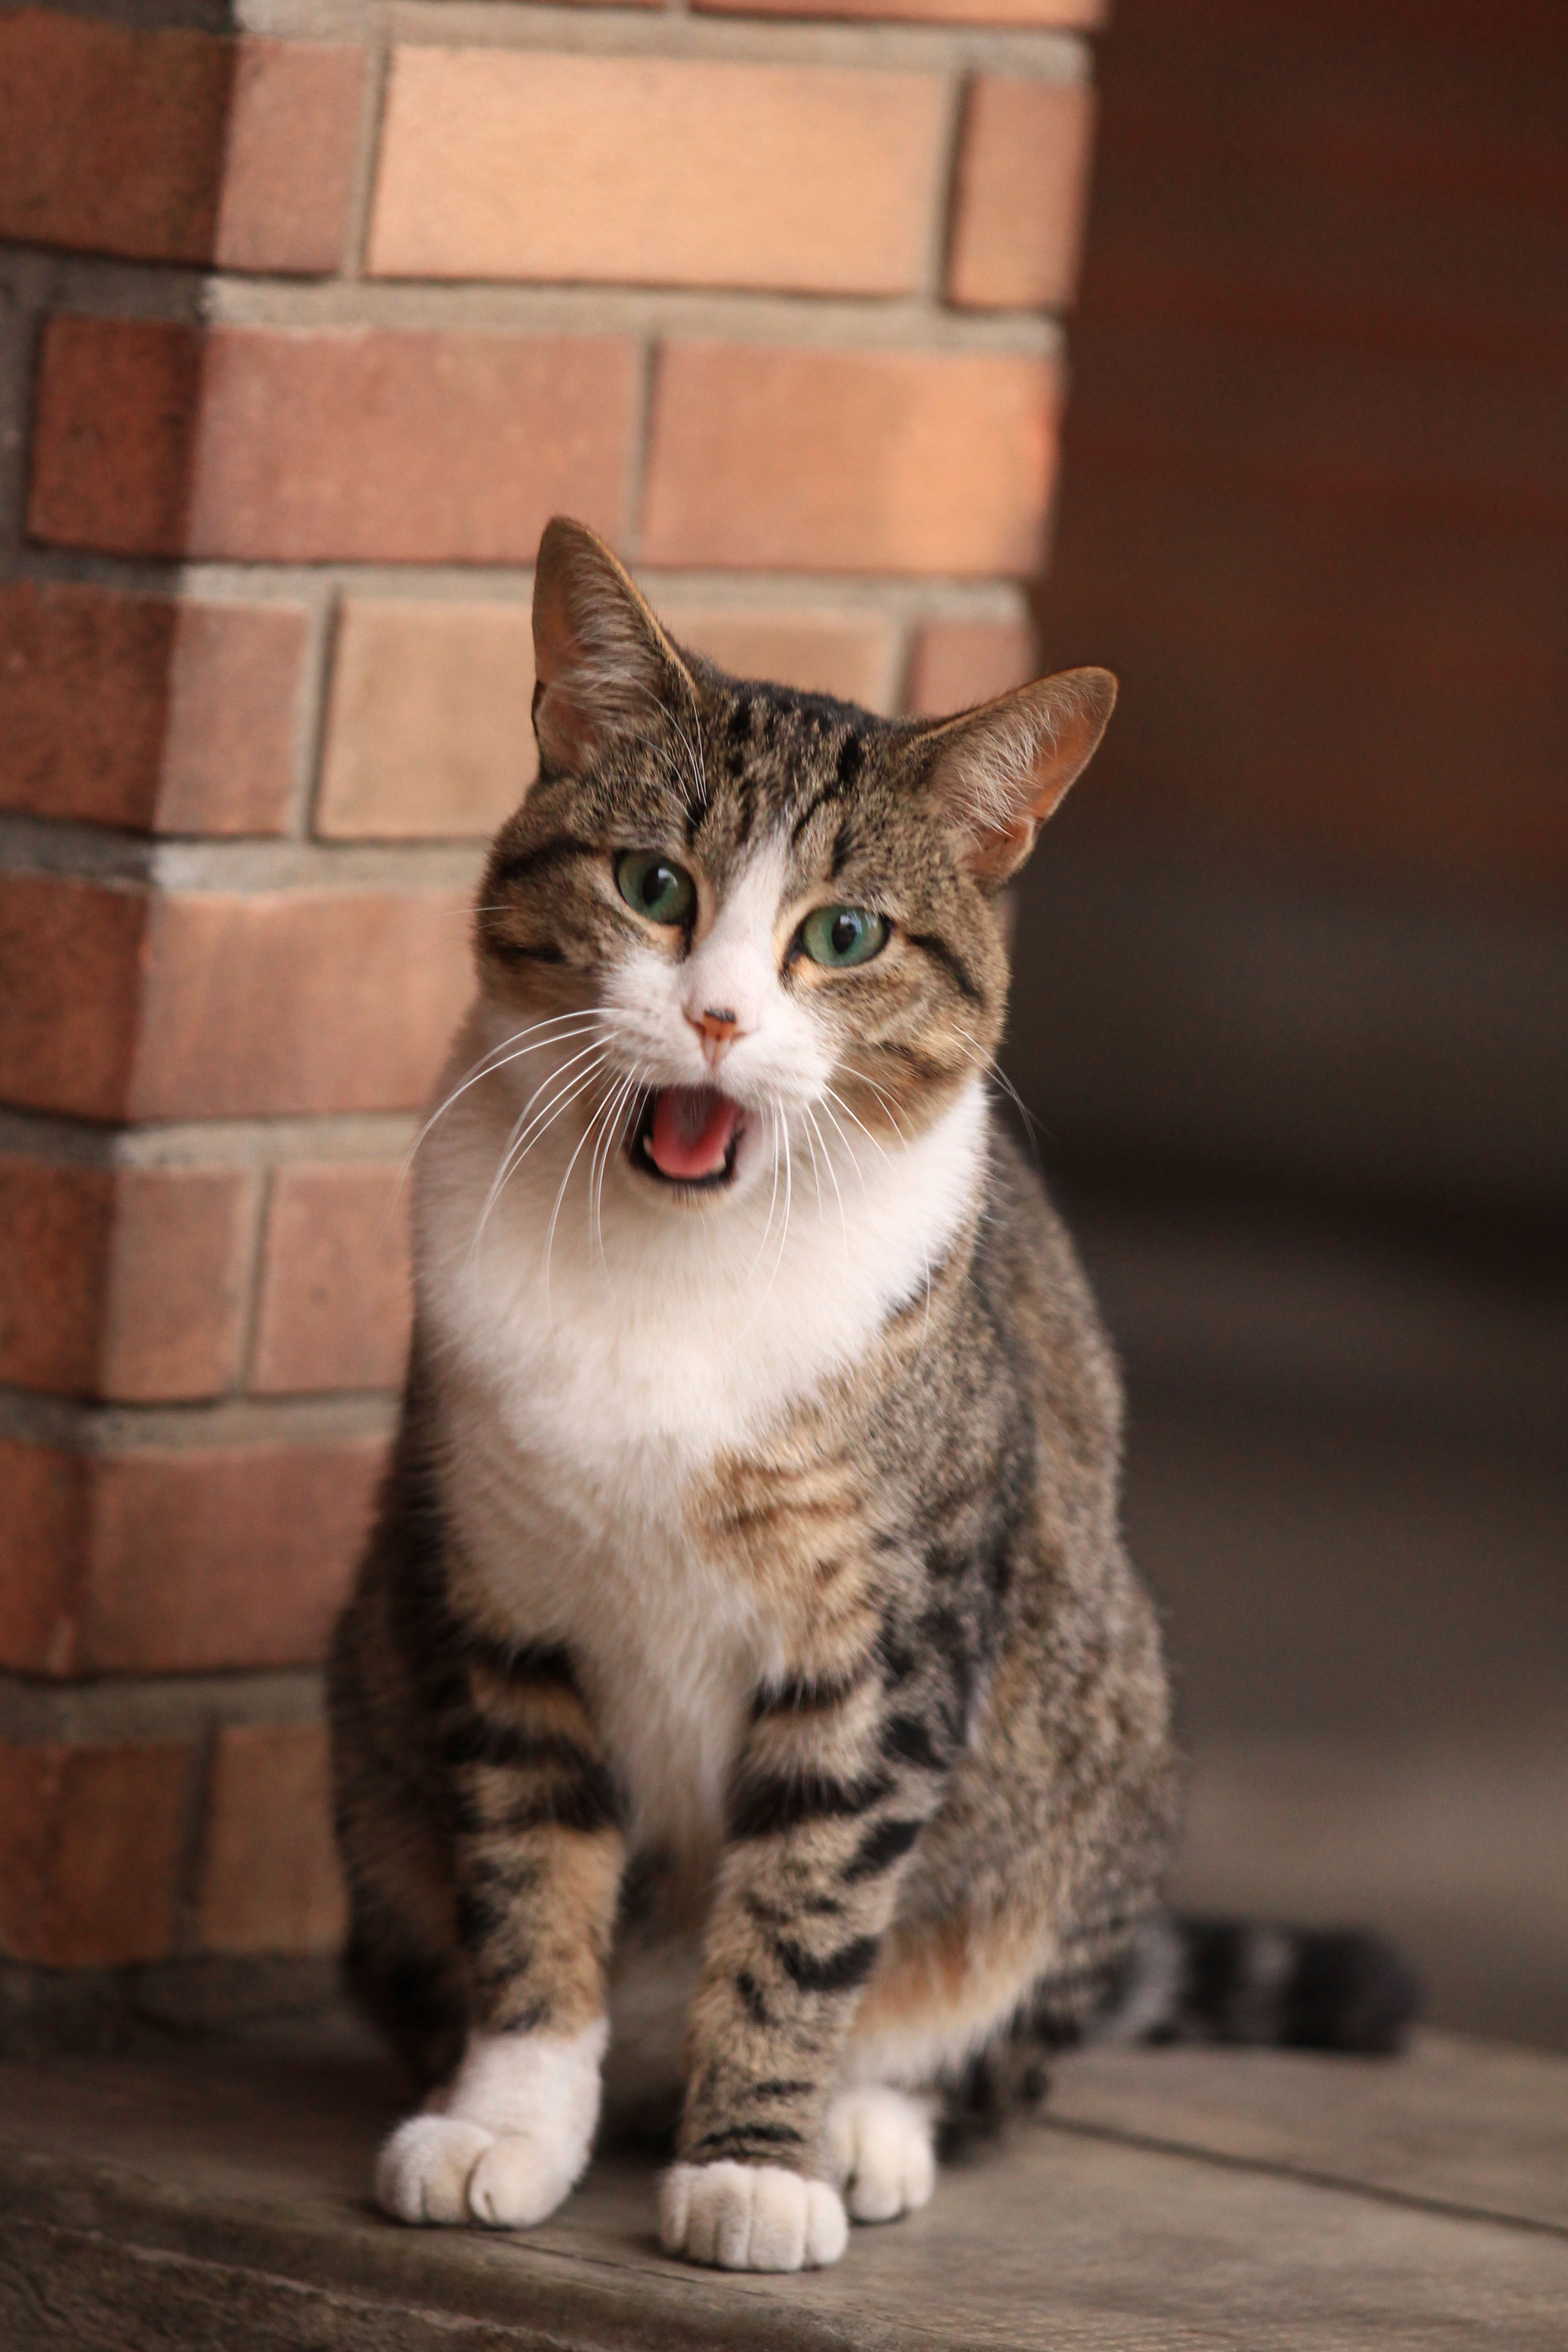
\includegraphics[width=52.5pt,height=78.73pt]{Bilder/European_cat_02_16_mp.jpg}};
%Shape: Square [id:dp7219434207477922] 
\draw  [fill={rgb, 255:red, 255; green, 0; blue, 0 }  ,fill opacity=1 ] (199.67,110) -- (299,110) -- (299,209.33) -- (199.67,209.33) -- cycle ;
%Straight Lines [id:da9021822569380376] 
\draw    (106.17,157.33) -- (177.17,157.33) ;
\draw [shift={(179.17,157.33)}, rotate = 180] [fill={rgb, 255:red, 0; green, 0; blue, 0 }  ][line width=0.75]  [draw opacity=0] (8.93,-4.29) -- (0,0) -- (8.93,4.29) -- cycle    ;

%Straight Lines [id:da9159956987115614] 
\draw    (337.17,157.33) -- (408.17,157.33) ;
\draw [shift={(410.17,157.33)}, rotate = 180] [fill={rgb, 255:red, 0; green, 0; blue, 0 }  ][line width=0.75]  [draw opacity=0] (8.93,-4.29) -- (0,0) -- (8.93,4.29) -- cycle    ;

%Straight Lines [id:da07325949392344144] 
\draw  [dash pattern={on 0.84pt off 2.51pt}]  (232.17,121.33) -- (277.17,121.33) ;


%Straight Lines [id:da9028616351053764] 
\draw  [dash pattern={on 0.84pt off 2.51pt}]  (233.17,196.33) -- (278.17,196.33) ;


%Straight Lines [id:da27535102010063794] 
\draw  [dash pattern={on 0.84pt off 2.51pt}]  (217.17,136.33) -- (217.17,184.33) ;


%Straight Lines [id:da9334949593538635] 
\draw  [dash pattern={on 0.84pt off 2.51pt}]  (286.17,133.33) -- (286.17,181.33) ;


%Straight Lines [id:da021722670153532242] 
\draw  [dash pattern={on 0.84pt off 2.51pt}]  (228.17,131.33) -- (278.17,183.33) ;


%Shape: Square [id:dp4109817022076603] 
\draw  [fill={rgb, 255:red, 255; green, 255; blue, 255 }  ,fill opacity=1 ] (449.67,90) -- (549,90) -- (549,189.33) -- (449.67,189.33) -- cycle ;
%Shape: Square [id:dp544671777438523] 
\draw  [fill={rgb, 255:red, 255; green, 255; blue, 255 }  ,fill opacity=1 ] (439.67,98) -- (539,98) -- (539,197.33) -- (439.67,197.33) -- cycle ;
%Shape: Square [id:dp9050599364199439] 
\draw  [fill={rgb, 255:red, 255; green, 255; blue, 255 }  ,fill opacity=1 ] (431.67,108) -- (531,108) -- (531,207.33) -- (431.67,207.33) -- cycle ;
%Straight Lines [id:da02360170094364733] 
\draw  [dash pattern={on 0.84pt off 2.51pt}]  (455.17,120.33) -- (500.17,120.33) ;


%Straight Lines [id:da10167634289204797] 
\draw  [dash pattern={on 0.84pt off 2.51pt}]  (455.17,194.33) -- (500.17,194.33) ;


%Straight Lines [id:da23003293896688182] 
\draw  [dash pattern={on 0.84pt off 2.51pt}]  (443.17,135.33) -- (443.17,183.33) ;


%Straight Lines [id:da28496973593396335] 
\draw  [dash pattern={on 0.84pt off 2.51pt}]  (521.17,134.33) -- (521.17,182.33) ;


%Straight Lines [id:da06739883279353798] 
\draw  [dash pattern={on 0.84pt off 2.51pt}]  (452.17,127.33) -- (514.17,183.33) ;



% Text Node
\draw (250,217) node  [align=left] {$\displaystyle 224$};
% Text Node
\draw (188.17,157.33) node [rotate=-270] [align=left] {$\displaystyle 224$};
% Text Node
\draw (314,202) node [rotate=-319.82] [align=left] {$\displaystyle 3$};
% Text Node
\draw (141,170) node  [align=left] {Resizing};
% Text Node
\draw (371,171) node  [align=left] {Normalization};
% Text Node
\draw (215.67,197.33) node  [align=left] {$\displaystyle 255$};
% Text Node
\draw (216,120) node  [align=left] {$\displaystyle 255$};
% Text Node
\draw (287,196) node  [align=left] {$\displaystyle 0$};
% Text Node
\draw (286,120) node  [align=left] {$\displaystyle 0$};
% Text Node
\draw (442.67,194.33) node  [align=left] {$\displaystyle 1$};
% Text Node
\draw (444,118) node  [align=left] {$\displaystyle 1$};
% Text Node
\draw (519,193) node  [align=left] {$\displaystyle -1$};
% Text Node
\draw (518,118) node  [align=left] {$\displaystyle -1$};
% Text Node
\draw (421.17,155.33) node [rotate=-270] [align=left] {$\displaystyle 224$};
% Text Node
\draw (484,215) node  [align=left] {$\displaystyle 224$};
% Text Node
\draw (546,203) node [rotate=-319.82] [align=left] {$\displaystyle 3$};
% Text Node
\draw (67,220) node  [align=left] {$\displaystyle 1633$};
% Text Node
\draw (22,153) node [rotate=-270.5] [align=left] {$\displaystyle 2449$};
% Text Node
\draw (69,98) node  [align=left] {{\scriptsize source: [SeL] }};


\end{tikzpicture}
\caption{Preprocessing steps for image classifcation: Resizing to the model input size and normalization of the pixel values to $[-1,1]$}
\label{fig:prepro}
\end{figure}
\paragraph{Edge Preprocessing}
\label{chap:preproImpl}
In the case of edge preprocessing all preprocessing steps are done on the edge device, meaning that the input can be fed directly into the neural network afterwards, either on the edge device itself or on a cloud-backend.
We perform these steps the following way: After loading the PNG image into an \emph{InputStream} we create a scaled Bitmap of the image (scaled to either $224\times224$ or $299\times299$) by calling the \emph{createScaledBitmap} function. 
Afterwards we normalize the RGB values to $[-1,1]$ during the conversion from the bitmap to a \emph{ByteBuffer}. 
For the case of float models this buffer contains all the pixels in float format and for quantized model in bytes, since quantized models work with lower represenations.
%%%mehr erklären?
We do this conversion since feeding \emph{ByteBuffers} to TensorFlow Lite is performance enhancing. %add cite here
For cloud inference we then construct \emph{PredictRequest} object containing this \emph{ByteBuffer}.

For batch size larger than one we parallize the preprocessing to speed up the proprocessing latency at the cost of higher maximum memory consumption. We start $n$ threads, where each thread is preprocessing one image in the way described above. After each image is preprocessed we concatenate all \emph{ByteBuffers} into a single one, which then can be fed to the TensorFlow Lite interpreter. Note that $n$ is determined by both batch size and available CPU cores on the edge device. There are never more threads than available cores, but if the batch size is smaller than the number of cores, we only start $n$ threads, where $n$ is the batch size. 

\paragraph{Cloud Preprocessing}

In the case of cloud inference the images can also be preprocessed directly on the cloud, resulting in nearly no preprocessing done on the edge. While the resizing and scaling steps are no longer done on the edge, the image still needs to converted into a \emph{PredictRequest} object that TensorFlow Serving can handle.
To achieve this we again load the PNG image into an \emph{InputStream}, convert it to a \emph{ByteArray} which then can be feed to the \emph{PredictRequest} object as a \emph{ByteString}. 

%Add TensorFlow Serving preprocessing here


\subsubsection{Inference}
To get the predictions for our now preprocessed image we need to run the inference operation of the inference framework with the deep learning model laoded, which is loaded either directly on the edge or on the remote cloud-backend. 
The inference is done using the steps described in section \ref{chap:TFLite} (TensorFlow Lite) and \ref{chap:TFServing} (TensorFlow Serving).
\paragraph{Edge Inference}
To perform the inference operation we two things into the \emph{run} function of an interpreter of TensorFlow Lite: The \emph{ByteBuffer} created in the preprocessing step and an array (float models: \emph{FloatArray}, quantized models: \emph{ByteArray}) with the length 1001 (number of classes). TensorFlow lite then writes the confidence levels of the different classes to this array. We then sort the array for the five classes with the highest confidence and print them to the screen.

\paragraph{Cloud Inference}

For the cloud inference we send the \emph{PredictRequest} object created in the preprocessing process to the TensorFlow Serving server, where the inference (and in the case of cloud preprocessing also the preprocessing) computations are executed.
To sent the \emph{PredictRequest} object to the server we call the \emph{predict} function of the previous created TensorFlow Serving gRPC stub.
Afterwards the client receives the \emph{PredictResponse} from the server containing the predictions for the sent image. We configured the TensorFlow Serving models to return the five classes with the highest confidence, hence we extract these five classes from the \emph{PredictResponse} and print them to the screen.

To preprocess the image on the cloud we add TensorFlows preprocessing functions to the model graphs before we export them to the TensorFlow Serving format. The images arrive at the server in the \emph{PNG} format, therefore we first decode them with \emph{tf.image.decode\_jpeg}, then resize with \emph{tf.image.resize\_bilinear} and finally normalize the tensor values to $[-1,1]$ using the the \emph{subtract} and \emph{multiply} functions. Now the input has the same shape as if they would have been preprocessed on the edge can be fed to the actual model graphs.
\section{Instantiation}
Using the experimental design presented in the previous section, we now describe which parameters we change in the course of the experiments as well as how the performance metrics are measured.
\subsection{Parameters}
We run each parameter configuration 15 times to reduce variance and stabilize our results.
During the experiments no other applications are running on either the edge or the cloud device.
In the course of the experiments we change the configurations of the following parameters:
%%%293,performance analysis buch
\paragraph{Model}
We conduct experiments for all three models listed presented in \ref{chap:models}: InceptionV4, MobileNetV2 and MobileNetV2 quantized.

\paragraph{Preprocessing Mode}
For the case of cloud inference the major parts of the needed preprocessing is either done on the edge before sending the image to the cloud or done on cloud. Therefore we evaluate both options.
\paragraph{Inference Mode}
The inference can either be performed on the edge or an a cloud-backend.

\paragraph{Image Size}
%%Add table here?
%224: 83KB
%299: 141KB
%2MP: 2411KB
%4MP: 4309KB
%8MP: 7515KB
%16MP: 10077KB
We evaluate the performance of 2MP($1732\times1155$, $2411$KB), 4MP($2449\times1633$, $4309$KB), 8MP($3464\times2309$, $7515$KB) and 16MP($4899\times3266$, $10077$KB) PNG images, as the OnePlus 6T is capable of taking pictures with 16 megapixel. This way the effect of different image sizes on the performance of the preprocessing step can assessed. We also evaluate an image where no resizing is needed ($224\times224$, $83$KB or $299\times299$, $141$KB depending on the model) to study the impact of image resizing. A picture of a cat (see figure \ref{fig:cat}) scaled to the different sizes will serve as the picture for the experiments.
\begin{figure}[H]
\centering
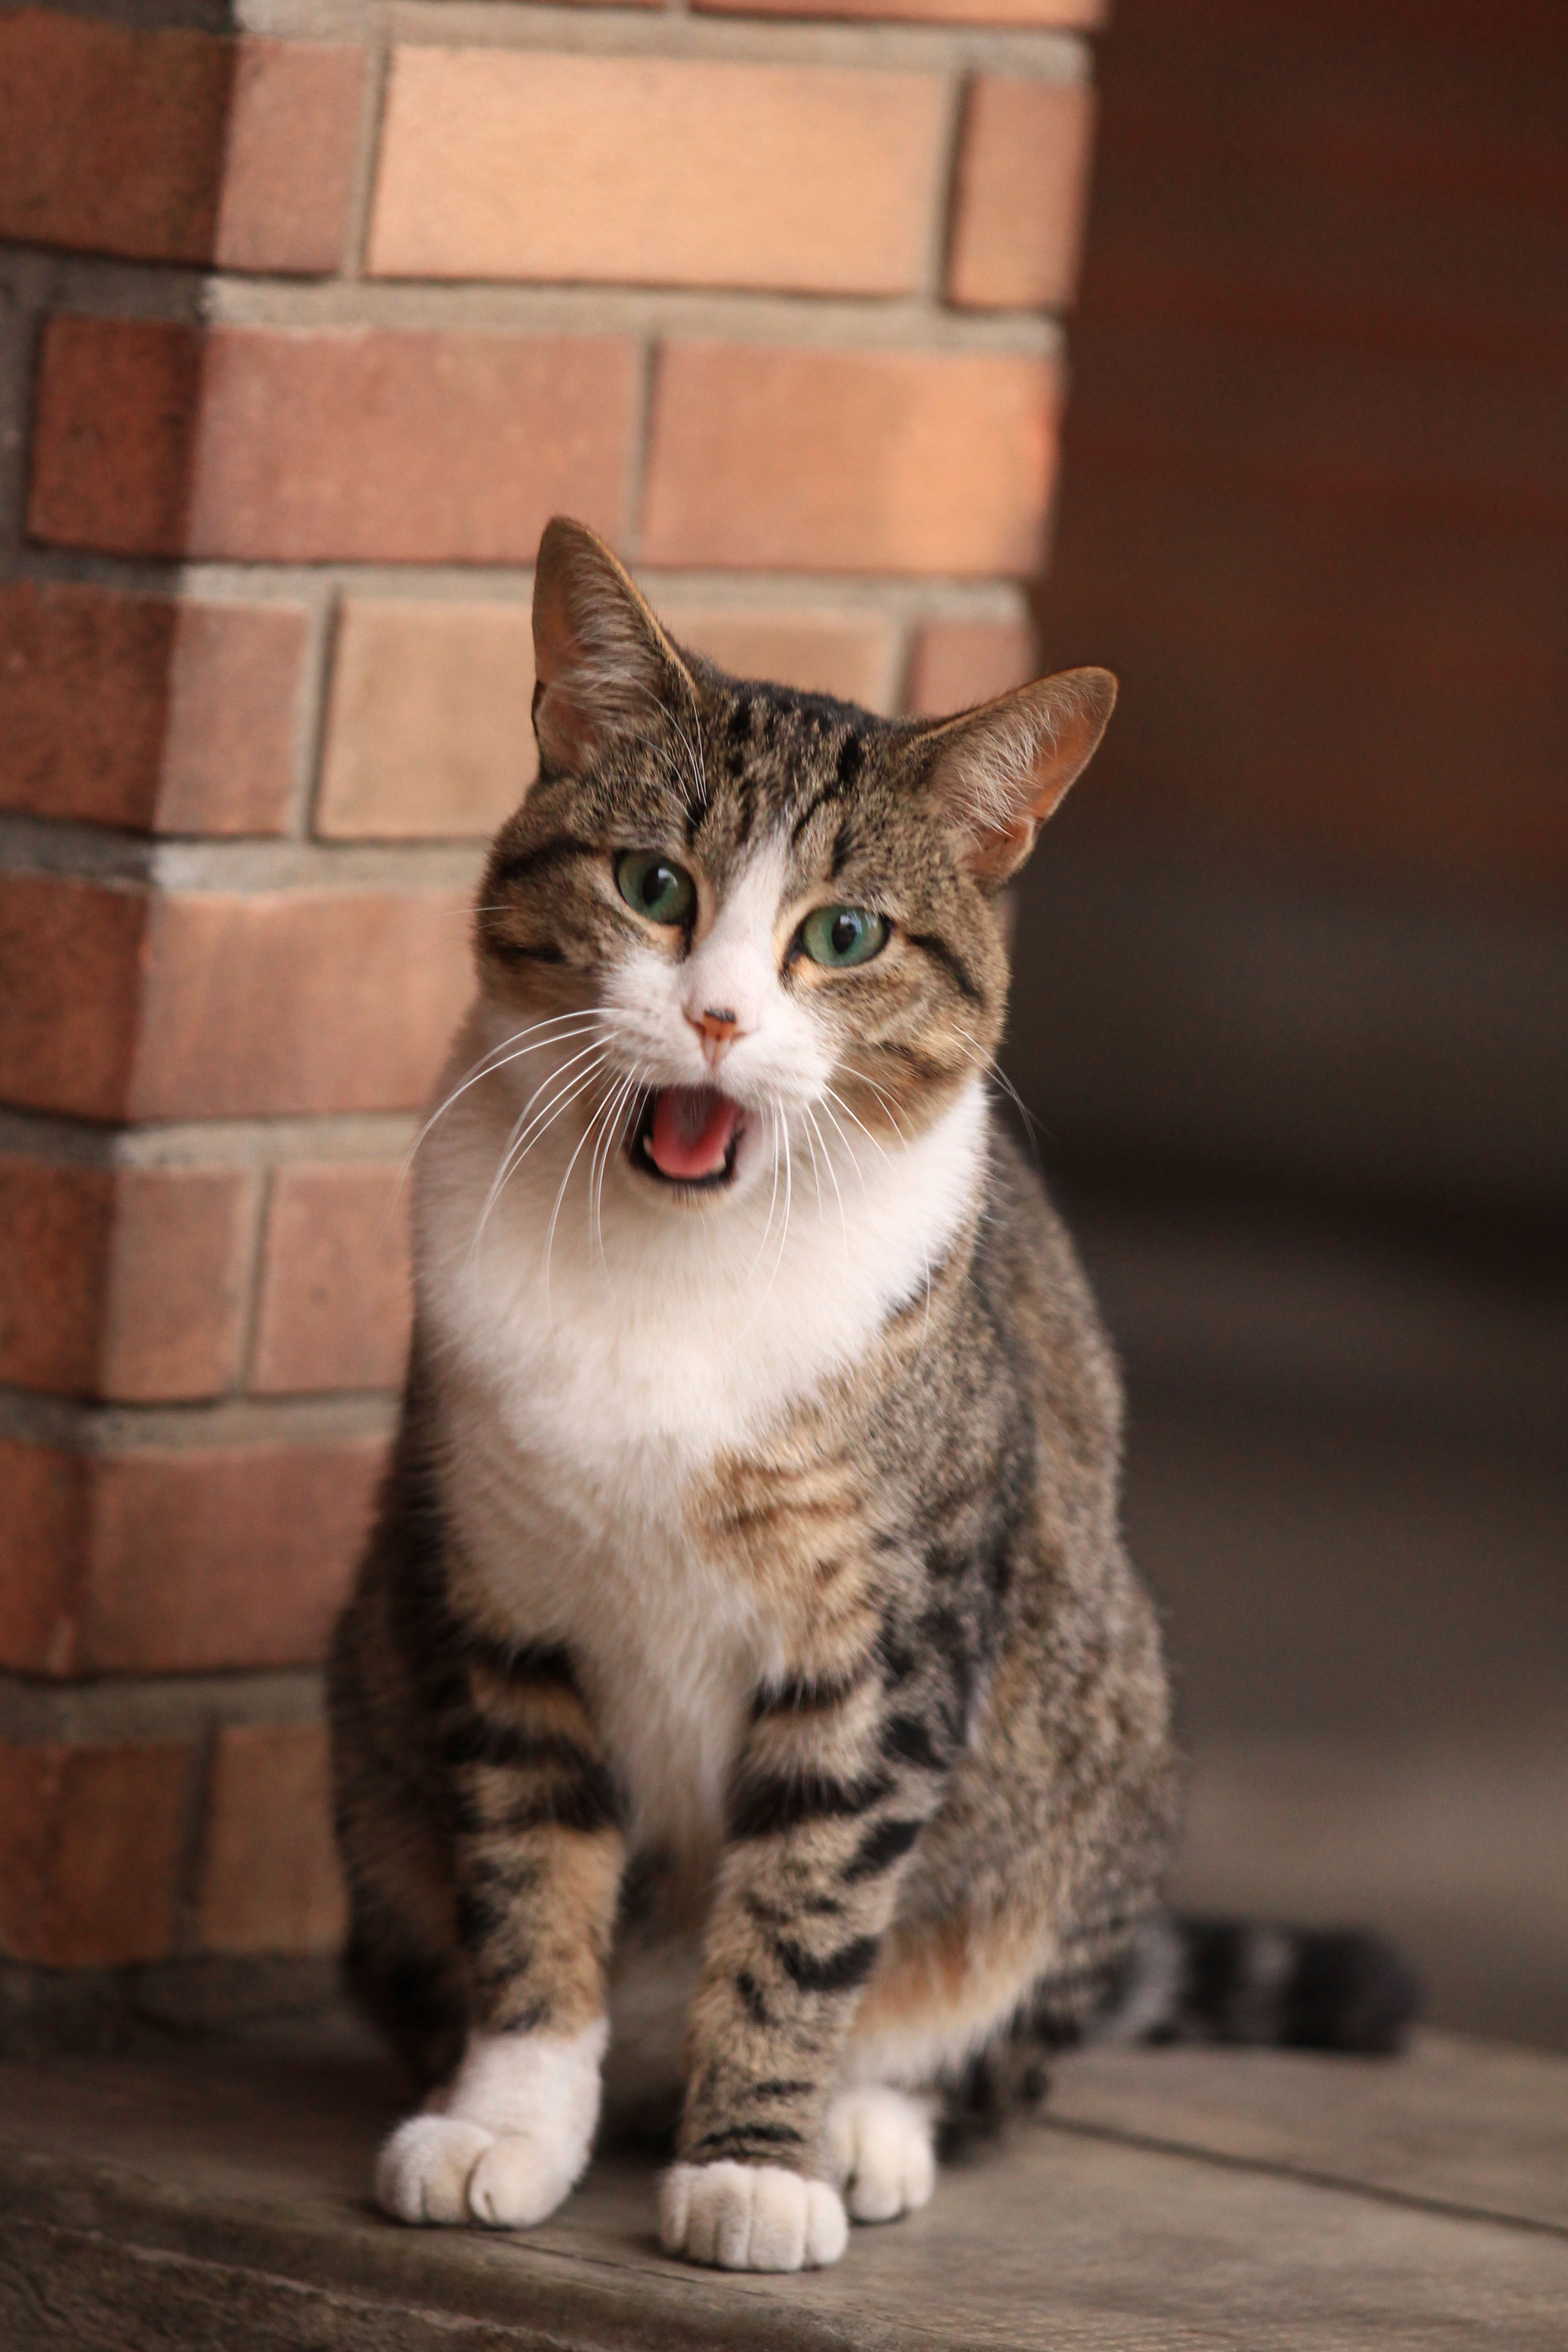
\includegraphics[width=0.3\textwidth]{./Bilder/European_cat_02_16_mp.jpg}
\caption{Picture used for the experiments \cite{cat}}
\label{fig:cat}
\end{figure}
\paragraph{Batch Size}
%%mathe defs of throughput?
Batch Size denotes the number of images fed into the deep learning model in a single inference operation. 
Feeding more than one image to the network can lead to a higher throughput, if enough computational power is available. This increase in throughput often comes at the cost of increased latency and general resource consumption.

To study these trade-offs we conduct experiments with the following batch sizes: 1, 2, 16, 32. Since at the point of these experiments a batch size greater than one is not supported for the TensorFlow Lite versions of MobilenetV2 (both float and quantized), measurements with these batch sizes cannot be performed for the case of edge inference at this point.
\paragraph{NNAPI}
The Android Neural Network API (NNAPI), presented in section \ref{chap:NNAPI}, is supposed to enhance the inference performance of TensorFlow Lite. Therefore we take a look into the effect of this framework.
%%Mention GPU use here
\paragraph{GPU Usage}
Since January 16 an experimental release of TensorFlow Lite supporting GPU usage on Android using OpenGL ES 3.1 Compute Shaders \cite{tfLiteGPU}.
So far only four public models and their operators are supported, including MobileNetV2, but not InceptionV4. 
Therefore we omit the test of this new feature in our experimentation, but our initial testing indicated that the use of NNAPI provides faster inference latencies for MobileNetV2 than the GPU version.
%%https://medium.com/tensorflow/tensorflow-lite-now-faster-with-mobile-gpus-developer-preview-e15797e6dee7
%experimental
%only mobilenet supported
%worse performance than NNAPI so far


\begin{figure}[H]
\centering
 \scalebox{.7}{%\documentclass[border=10pt]{standalone}
%\usepackage{tikz}
%\begin{document}
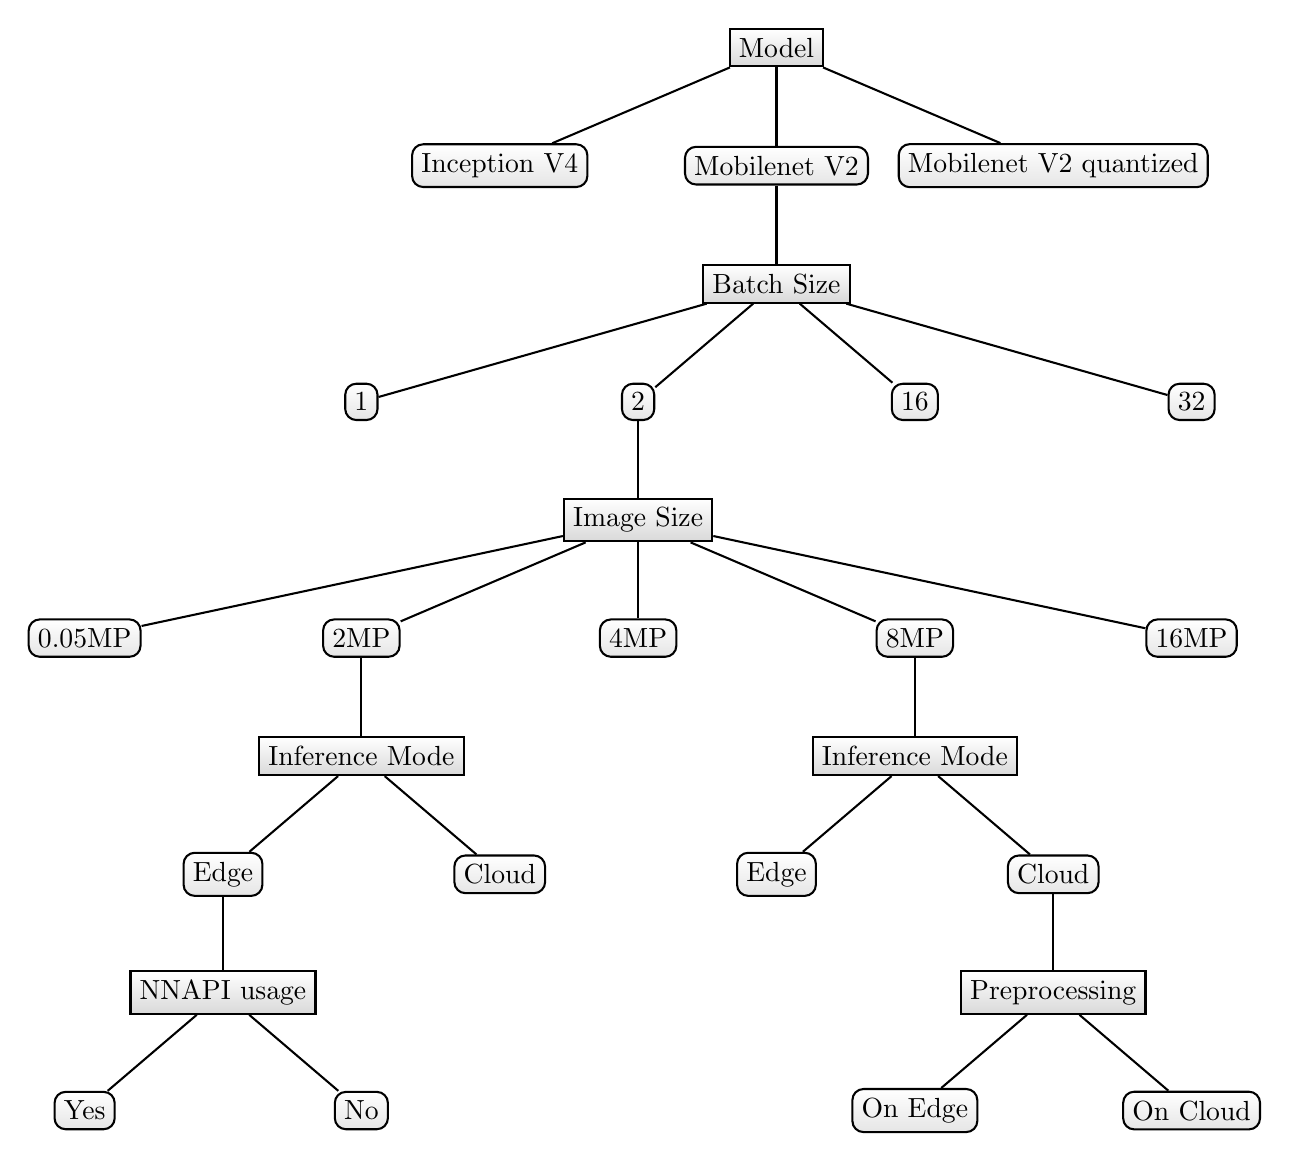
\begin{tikzpicture}[sibling distance=10em,
  param/.style={shape=rectangle,
    draw, align=center,
    top color=white, bottom color=gray!30},
  conf/.style={shape=rectangle, rounded corners,
    draw, align=center,
    top color=white, bottom color=gray!20}  ]  ]
    
  \node[param] {Model}
    child { node [conf]{Inception V4} }
    child { node [conf]{Mobilenet V2}
      child { node [param]{Batch Size}
        child { node [conf]{1} }
        child { node [conf]{2} 
            child { node [param]{Image Size}
                child { node [conf]{0.05MP}}
                child { node [conf]{2MP}
                child { node [param]{Inference Mode}
                        child { node[conf] {Edge}
                            child { node[param] {NNAPI usage}
                                 child { node[conf] {Yes}}
                                 child { node [conf]{No}}}}
                        child { node [conf]{Cloud}
                            }}}
                child { node [conf]{4MP}
                    }
                child { node [conf]{8MP}
                child { node [param]{Inference Mode}
                        child { node[conf] {Edge}}
                        child { node [conf]{Cloud}
                            child { node [param]{Preprocessing}
                               child { node [conf]{On Edge}}
                                child { node [conf]{On Cloud}}}}}}
                child { node [conf]{16MP}}}}
        child { node[conf] {16} }
        child { node [conf]{32} }} }
    child { node [conf]{Mobilenet V2 quantized} };
\end{tikzpicture}
%\end{document}}

\caption{Excerpt of the performed experiments configurations}
\label{fig:tree}
\end{figure}
Figure \ref{fig:tree} shows a part of our experimentation tree. In theory there would be 240 different parameter configurations, but due to a number of reasons the number of different configurations reduced to 113 in total.

First, the Usage of NNAPI is independent of the image size hence we only perform experiments without NNAPI for a single image size. Also the usage of NNAPI leads to a way better performance for edge inference and we want to compare edge and cloud inference, so we only carry out experiments without NNAPI for a batch size of one.
We omit the cloud inference for the quantized MobileNetV2 because the model is so small the network overhead would be overwhelming.%INSERT REASON.

%of limited capacity/time and
Lastly due to lack of support certain operations in TensorFlow Lite for the MobileNetV2 models, we can not perform inference experiment for MobileNetV2 with a batch size larger than one.
\subsection{Performance Metrics}
\label{chap:insta_measurements}
In the following section we describe how we measure the performance metrics defined in \ref{chap:metrics}.
We conduct the measurements either directly in the source code or by using Android Studio Profiler (Version 3.3). Since Android Studio cannot collect all metrics the way we wanted, we wanted to used Trepn as a secondary profiling application. But since Trepn does not support our test device, we had to omit these metrics.

In the following definitions $t_{start}$ denotes the starting point of either the preprocessing or inference, while $t_{end}$ denotes the end point of the respective process.
\subsubsection{Latency}
We measure $Latency_{preprocessing}$ by measuring the time difference between start and end of the preprocessing process.
Note that all latency measurements are reported in milliseconds(ms).
\begin{equation*}
\begin{gathered}
Latency_{preprocessing} = t_{endPreprocessing} - t_{startPreprocessing}
\end{gathered}
\end{equation*}
To measure inference latency we need to distinguish between edge and cloud inference, since for the latter the network latency needs to be considered.

\paragraph{Edge Inference}To measure edge inference latency we measure the time the TensorFlow Lite interpreter needs to run the inference operation on the loaded model given the input image.
\begin{equation*}
\begin{gathered}
Latency_{inference} = t_{endInference} - t_{startInference}
\end{gathered}
\end{equation*}
\paragraph{Cloud Inference}
To measure the cloud inference latency we need to measure two latencies, which combined yield $Latency_{inference}$. The first latency is  $Latency_{server}$. This server latency describes the time difference between the point where TensorFlow Serving receives the inference request and the point in time where TensorFlow Serving sends the response back to the client.
The second latency $Latency_{network}$ denotes the time the prediction request needs to reach the cloud-backend.
These latencies are illustrated in figure \ref{fig:serverLat}.
\begin{figure}[!htb]
\centering


\tikzset{every picture/.style={line width=0.75pt}} %set default line width to 0.75pt        

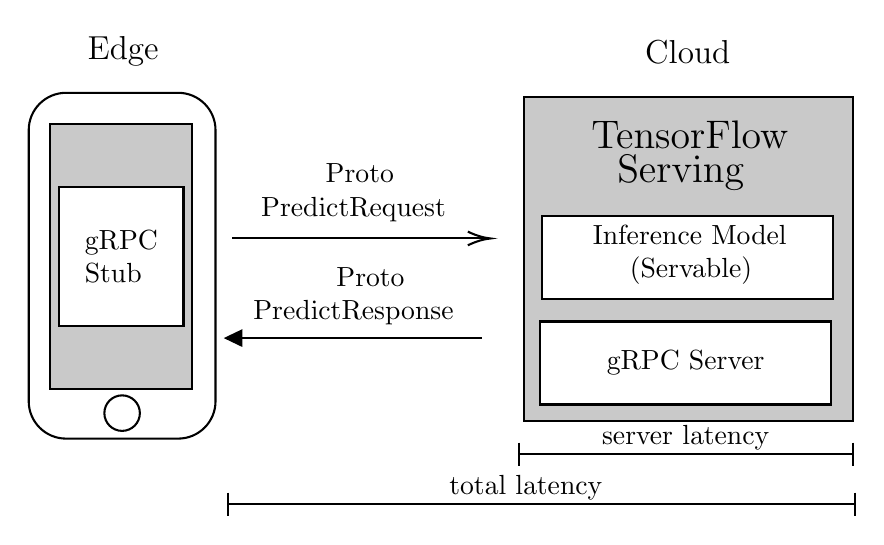
\begin{tikzpicture}[x=0.75pt,y=0.75pt,yscale=-1,xscale=1]
%uncomment if require: \path (0,300); %set diagram left start at 0, and has height of 300

%Straight Lines [id:da7072764839644827] 
\draw    (149.5,277) -- (451.5,277) ;
\draw [shift={(451.5,277)}, rotate = 180] [color={rgb, 255:red, 0; green, 0; blue, 0 }  ][line width=0.75]    (0,5.59) -- (0,-5.59)   ;
\draw [shift={(149.5,277)}, rotate = 180] [color={rgb, 255:red, 0; green, 0; blue, 0 }  ][line width=0.75]    (0,5.59) -- (0,-5.59)   ;
%Straight Lines [id:da9536138531960994] 
\draw    (289.5,253) -- (450.5,253) ;
\draw [shift={(450.5,253)}, rotate = 180] [color={rgb, 255:red, 0; green, 0; blue, 0 }  ][line width=0.75]    (0,5.59) -- (0,-5.59)   ;
\draw [shift={(289.5,253)}, rotate = 180] [color={rgb, 255:red, 0; green, 0; blue, 0 }  ][line width=0.75]    (0,5.59) -- (0,-5.59)   ;
%Shape: Rectangle [id:dp8902536871651789] 
\draw  [fill={rgb, 255:red, 201; green, 201; blue, 201 }  ,fill opacity=1 ] (63.91,93.69) -- (132.34,93.69) -- (132.34,221.63) -- (63.91,221.63) -- cycle ;
%Rounded Rect [id:dp41557214204551274] 
\draw   (53.5,96.82) .. controls (53.5,86.88) and (61.56,78.82) .. (71.5,78.82) -- (125.5,78.82) .. controls (135.44,78.82) and (143.5,86.88) .. (143.5,96.82) -- (143.5,227.43) .. controls (143.5,237.37) and (135.44,245.43) .. (125.5,245.43) -- (71.5,245.43) .. controls (61.56,245.43) and (53.5,237.37) .. (53.5,227.43) -- cycle ;
%Shape: Ellipse [id:dp8878397246816687] 
\draw   (89.95,233.16) .. controls (89.95,228.43) and (93.78,224.6) .. (98.5,224.6) .. controls (103.22,224.6) and (107.05,228.43) .. (107.05,233.16) .. controls (107.05,237.88) and (103.22,241.71) .. (98.5,241.71) .. controls (93.78,241.71) and (89.95,237.88) .. (89.95,233.16) -- cycle ;
%Straight Lines [id:da5813802620369573] 
\draw    (151.48,149) -- (274,149) ;
\draw [shift={(276,149)}, rotate = 540] [color={rgb, 255:red, 0; green, 0; blue, 0 }  ][line width=0.75]    (10.93,-3.29) .. controls (6.95,-1.4) and (3.31,-0.3) .. (0,0) .. controls (3.31,0.3) and (6.95,1.4) .. (10.93,3.29)   ;

%Straight Lines [id:da16220168680973557] 
\draw    (149.48,197) -- (272,197) ;

\draw [shift={(147.48,197)}, rotate = 360] [fill={rgb, 255:red, 0; green, 0; blue, 0 }  ][line width=0.75]  [draw opacity=0] (8.93,-4.29) -- (0,0) -- (8.93,4.29) -- cycle    ;
%Shape: Rectangle [id:dp8411150472244695] 
\draw  [fill={rgb, 255:red, 201; green, 201; blue, 201 }  ,fill opacity=1 ] (292,81) -- (450.5,81) -- (450.5,237) -- (292,237) -- cycle ;
%Shape: Rectangle [id:dp13557861576626729] 
\draw  [fill={rgb, 255:red, 255; green, 255; blue, 255 }  ,fill opacity=1 ] (301,138) -- (441,138) -- (441,178) -- (301,178) -- cycle ;
%Shape: Rectangle [id:dp5681963435258506] 
\draw  [fill={rgb, 255:red, 255; green, 255; blue, 255 }  ,fill opacity=1 ] (68.19,124.22) -- (128.07,124.22) -- (128.07,191.1) -- (68.19,191.1) -- cycle ;
%Shape: Rectangle [id:dp7458124222136935] 
\draw  [fill={rgb, 255:red, 255; green, 255; blue, 255 }  ,fill opacity=1 ] (300,189) -- (440,189) -- (440,229) -- (300,229) -- cycle ;

% Text Node
\draw (370,245) node  [align=left] {server latency};
% Text Node
\draw (293,269) node  [align=left] {total latency};
% Text Node
\draw (210,127) node  [align=left] { \ \ \ \ \ \ \ Proto\\PredictRequest};
% Text Node
\draw (99,59) node  [align=left] {{\large Edge}};
% Text Node
\draw (371,59) node  [align=left] {{\large Cloud}};
% Text Node
\draw (372,109) node  [align=left] {{\Large TensorFlow}\\{\Large  \ \ Serving}};
% Text Node
\draw (372,157) node  [align=left] {Inference Model\\ \ \ \ \ (Servable)};
% Text Node
\draw (210,177) node  [align=left] { \ \ \ \ \ \ \ \ \ Proto\\PredictResponse};
% Text Node
\draw (98.13,157.66) node  [align=left] {gRPC\\ Stub};
% Text Node
\draw (370,209) node  [align=left] {gRPC Server};


\end{tikzpicture}
\caption{Measurement of $Latency_{server}$ and $Latency_{network}$ for Cloud Inference}
\label{fig:serverLat}
\end{figure}


Similar to the edge inference, $Latency_{inference}$ is being measured by calculating the time difference between starting the inference process and receiving the prediction for the given inference request. This whole process is covered by the \emph{predict} function of TensorFlow Serving. Therefore we measure the wall clock time of this function.

Since TensorFlow Serving does not output the server latency, we needed to tweak the source code of gRPC, which is the underlying protocol of TensorFlow Serving. gRPC already logs this latency, so we adjust the source code to output this latency when a call to TensorFlow Serving is finished, repackage the source code and change to dependencies of TensorFlow Serving pointing to the adjusted packages.

We then calculate $Latency_{network}$ implicitly by subtracting $Latency_{server}$ from $Latency_{inference}$.

\begin{equation*}
\begin{gathered}
Latency_{inference} = t_{endInference} - t_{startInference}\\
Latency_{server}= t_{receive Request} - t_{send Response}\\
Latency_{network} = Latency_{inference} - Latency_{server}
\end{gathered}
\end{equation*}


The total latency $Latency_{total}$ for both edge and cloud inference is simply calculated by summing up the latencies of both preprocessing and inference.
\begin{equation*}
\begin{gathered}
Latency_{total} = Latency_{preprocessing} + Latency_{inference}
\end{gathered}
\end{equation*}
\subsubsection{Energy Consumption}
Since Android Studio Profiler only estimates the energy consumption in the form of low, medium and high, the tool is not fit to provide empiric measurements. The Trepn Power Profiler would provide such measurements, but does not support the device used for the experiments (OnePlus 6T).
\subsubsection{CPU Usage}
We measure the CPU usage(\%) of both preprocessing as the maximum CPU usage during the respective processes.
\begin{equation*}
\begin{gathered}
%%CPU_{preprocessing} = max_{[start_{preprocessing}, end_{preprocessing}]}(CPU)\\
%%CPU_{inference} = max_{[start_{inference}, end_{inference}]}(CPU)\\
CPU_{preprocessing} = \max\limits_{t_{startPreprocessing} \leq t \leq t_{endPreprocessing}} CPU_{Usage}(t)\\
CPU_{inference} = \max\limits_{t_{startInference} \leq t \leq t_{endInference}} CPU_{Usage}(t)
\end{gathered}
\end{equation*}
Android Studios’ CPU Profiler allows us to record the maximum CPU usage for both preprocessing and inference. To minimize the impact on the Android Profiler on the performance of the application we disable allocation tracking.
\begin{figure}[H]
\centering  
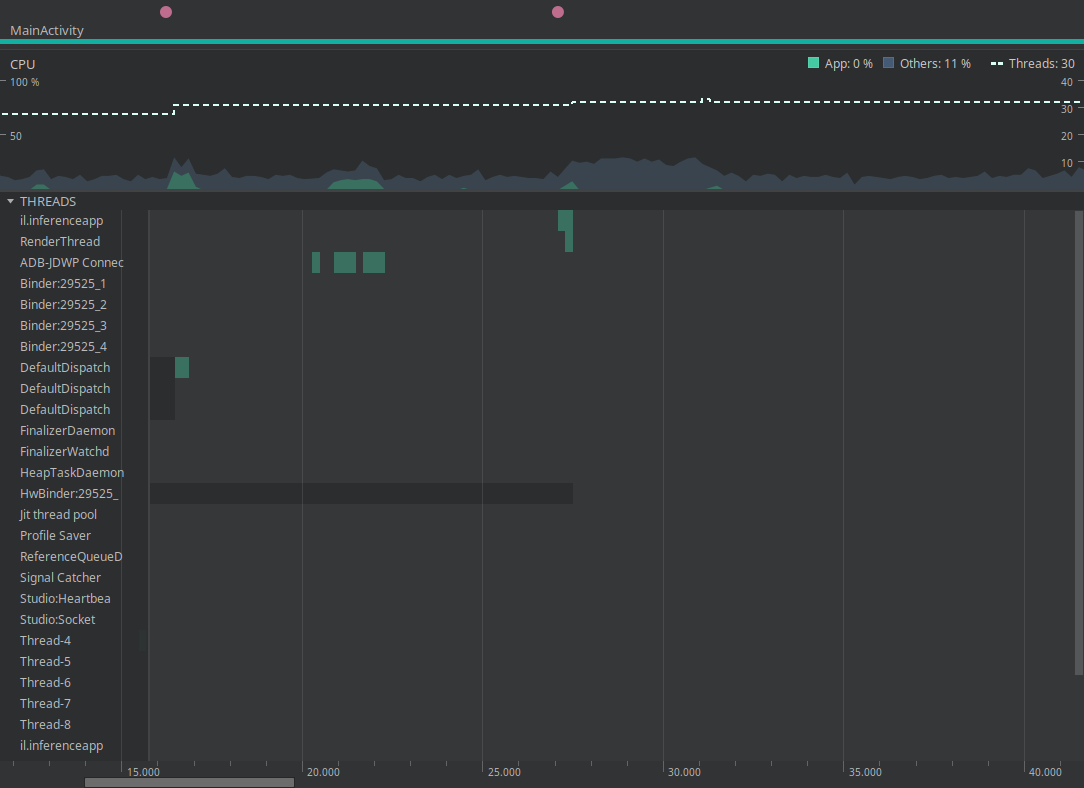
\includegraphics[width=0.6\textwidth]{./Bilder/profiler_CPU}
\caption{Android CPU Profiler}
\label{fig:prof_cpu}
\end{figure}
\subsubsection{Memory Usage}
We measure the memory usage by recording the maximum memory consumption during both processing and inference. Both of the following metrics are reported in megabytes(MB) in the result section.
\begin{equation*}
\begin{gathered}
Memory_{preprocessing} = \max\limits_{t_{startPreprocessing} \leq t \leq t_{endPreprocessing}} Memory(t)\\\\
Memory_{inference} = \max\limits_{t_{startInference} \leq t \leq t_{endInference}} Memory(t)\\
\end{gathered}
\end{equation*}
The Memory Profiler is part of Android Studio Profiler and shows the memory consumption of the app it is profiling. Memory allocations by the operating system or other apps are not recorded. Besides recording the total amount of memory allocated the Profiler also tracks the different categories, for example memory allocated by Java/Kotlin code. We always record the maximum consumed memory for each operation.
%%memory not accurate over 1GB
Note that for values greater than $1000$MB the profiler only reports gigabyte values with one decimal place. For example the profiler reports $1410$MB as $1.4$GB.

Figure \ref{fig:prof_mem} depicts an example of the Memory Profiler for a single experiment. The first peak in memory consumption is the preprocessing step, while the second peak is caused by the inference process.
The little trash can at the bottom of the figure shows that the garbage collection was called. The garbage collection was always manually called after the preprocessing in case not all unneeded memory allocations are collected before running the inference operation. 
Note that we report total memory consumption of the application, including memory consumed for the graphical interface or the \emph{Logger} class.
%In the case of preprocessing only the preprocessed image is needed, so the 
\begin{figure}[H]
\centering
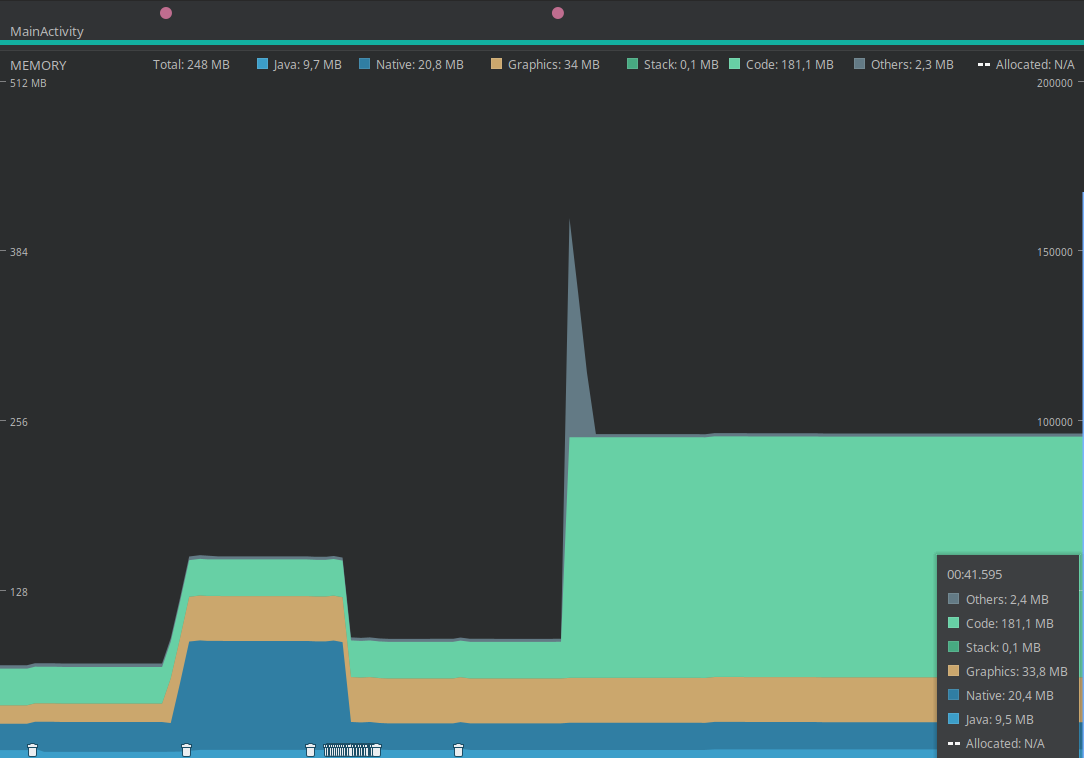
\includegraphics[width=0.6\textwidth]{./Bilder/profiler_MEM}
\caption{Android Memory Profiler showing the memory consumption during preprocessing and inference}
\label{fig:prof_mem}
\end{figure}
\subsubsection{GPU Usage}
Neither Android Studio nor Trepn can provide GPU metrics for the OnePlus 6T. Hence no GPU measurements can be conducted.
\subsubsection{Throughput}
We differentiate three types of throughput: the inference throughput, preprocessing throughput and the total throughput, which also includes preprocessing besides inference.
We calculate throughput in operations per second by 

\begin{equation*}
\begin{gathered}
Throughput_{preprocessing} =\frac{1000}{(Latency_{preprocessing}) / batchsize}\\
Throughput_{inference} =\frac{1000}{(Latency_{inference}) / batchsize}\\
Throughput_{total}  =\frac{1000}{(Latency_{total}) / batchsize}
\end{gathered}
\end{equation*}
\subsubsection{Data Consumption}
We measure both transmitted and received data by using the Android TrafficStats package (https://developer.android.com/reference/android/net/TrafficStats). We start measuring both transmitted and received bytes when the inference operation is started and stop when the response from the server is returned. We report both $Data_{transmitted}$ and $Data_{received}$ in kilobytes(KB).
\begin{equation*}
\begin{gathered}
Data_{transmitted} = \sum_{t_{startInference}}^{t_{endInference}} Data_{transmitted}(t)\\
Data_{received} = \sum_{t_{startInference}}^{t_{endInference}} Data_{received}(t)
\end{gathered}
\end{equation*}
\section{Results and Evaluation}
The previous section covered the experimental design, including used models, hardware devices and framework, as well as definition of performance metrics. Using this design specifications, we will now present and evaluate the results of the conducted experiments.

First, we take a look into the individual results of edge and cloud inference and afterwards compare them against each other. In each of these sections first the preprocessing and then the inference results are presented. 
In the last subsection we take a seperate look at batch sizes larger than one.

%die 83mb aufschlüsseln in GUI etc 
%Logger verbrauch erwähnen
Note that the Android application consumed around 83MB in memory and 0\% CPU during idle. Additionally the logger, which is used to save the measurements of the experiments consumes memory as well, hence the memory consumption shown in the results include both logger and other memory overhead caused by the graphical interface etc.

For precise mean values and standard deviations of all measured metrics refer to tables \ref{measurementsInception} and \ref{measurementsMobilenet}.

The black bar on top of each bar of the following bar chart and translucent areas around the lines of the line plots represent the standard deviation.

Preprocessing is performed without any models loaded on the edge. but with the image loaded into memory before the start of preprocessing to prevent the I/O operations to influence the preprocessing performance.
Edge Inference is done using a loaded model. We do not consider model loading latency in this thesis.

All experiments are done using the eduroam Wi‑Fi, since the cloud-backend server hosted at the LRZ is only reachable within the Münchner Wissenschaftsnetz (MWN) and a VPN would have an impact on network latencies.

We conducted the experiments in multiple sessions, where each session consists of $100$ experiments distributed over about two hours, thus preventing the results to be skewed by thermal throttling.
\subsection{Edge Inference}
This section covers the results of the edge inference experiments with OnePlus 6T device presented in section \ref{chap:hardwareEdge}.

Note that this section only covers the results for a batch size of one, for the results of larger batch sizes please refer to section \ref{chap:resultsBatchSize}.

\FloatBarrier
\subsubsection{Preprocessing}
\label{chap:edgePrepro}
Figure \ref{fig:EdgePrepro} shows the $Latency_{preprocessing}$ and $Memory_{preprocessing}$ for the different image sizes and models.

There is little difference in both latency and memory for the different models. 
InceptionV4 uses on average $7.5$MB more memory (or $5\%$) than the MobileNetV2 models, which is caused by the models higher input size (InceptionV4 $299\times299$, MobileNetV2 $224\times224$). 
These small differences are expected, since both all three model require roughly the same input specifications, with the exception of input size, but the difference between the two input sizes is relatively small.

While the different models have little difference in memory and latency, the image size has an significant impact on both of these metrics.
A $16$ megapixel image takes on average across all models more than $10$ times as long to preprocess as well as using $1.5$ times more memory in comparison to a $224^2/299^2$ image.
Figure \ref{fig:EdgePrepro} shows a steady increase of $Latency_{preprocessing}$ and $Memory_{preprocessing}$ across the increasing image sizes.
Preprocessing of large images is therefore mainly affected by the resizing process, not the pixel normalization or conversion to a \emph{ByteBuffer}, since these steps are performed after the resizing, thus having the same impact on performance as they would have on an $224^2/299^2$ image.

The standard deviation of both memory and latency are both low, indicating a stable resource consumption.


%%factors reinbringen auch kb größe der bilder
%%mehr impact on latency than memory

\begin{figure}[!htb]
\centering
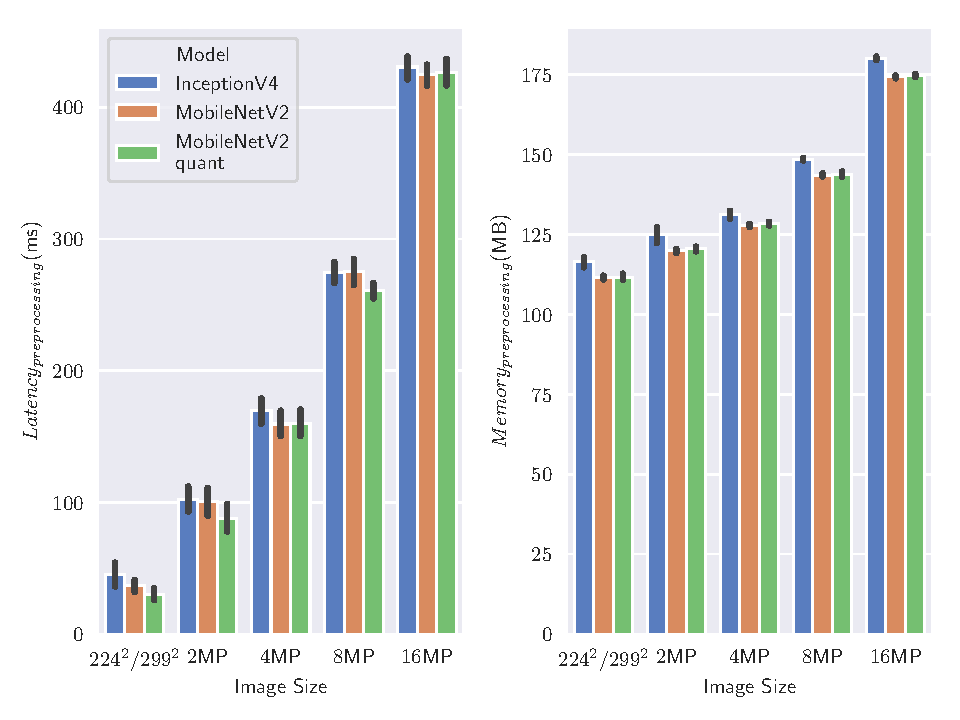
\includegraphics[width=0.8\textwidth]{./Bilder/single_plots/edge_inference_plots/Edge_Inference_Preprocessing.pdf}
\caption[Edge Inference: Preprocessing $Latency_{preprocessing}$, $Memory_{preprocessing}$]{Edge Inference: Preprocessing $Latency_{preprocessing}$, $Memory_{preprocessing}$ -  lower is better: Increasing image sizes have increasing impact on both memory and latency, independent of model type}
\label{fig:EdgePrepro}
\end{figure}
%%Was über CPU hier sagen
%%CPU usage in obere grafik integrieren?
Looking the CPU usages during preprocessing (see figure \ref{fig:CloudEdgePreproCPU}) one can see that the usages are very similar across all models and image sizes. This is probably due to the fact that the preprocessing of a single image is done on a single core. Since the OnePlus 6T has $8$ cores, the maximal CPU usage cause by a single core is $12.5\%$, which also is displayed in the plot, where all usages are close to this number.
%%High variance
%%around?

\FloatBarrier
\subsubsection{Inference}
This section presents the results for edge inference, in particular the effect of the Android Neural Network API.
Different image sizes have no effect on edge inference, as image are always preprocessed when they reach the inference step.
Hence we do not consider the different image sizes in the majority of this section.


\begin{comment}
\begin{figure}[H]
\centering
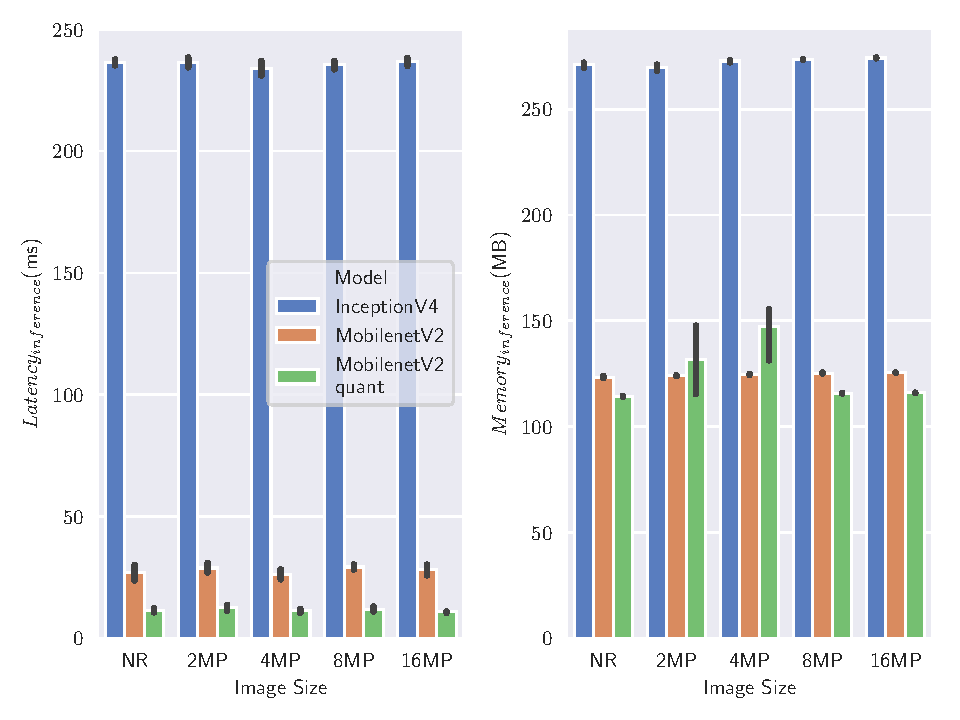
\includegraphics[width=0.8\textwidth]{./Bilder/single_plots/edge_inference_plots/Edge_Inference_Inference.pdf}
\caption{Edge Inference: Inference metrics - lower is better}
\label{fig:EdgeInference}
\end{figure}


\end{comment}
\subsubsection{Effect of NNAPI}
%%effcient
The Android Neural Network API (NNAPI) is supposed to speed up inference of neural network on Android by introducing optimised kernels/operators. 
The effect of this framework can be seen in figure \ref{fig:NNAPI} and show the significant performance improvement caused by the NNAPI, not only affecting $Latency_{inference}$, but also $Memory_{inference}$ and $CPU_{inference}$.

%%Genauere factors einfügen : inferecen zweimal so schnell...
This effect can be observed across all tested models, but especially on the InceptionV4 network.

Note that the NNAPI uses the GPU of the OnePlus 6T for a part of its inference, therefore while reducing the CPU usage during inference, the NNAPI probably causes higher GPU usages.

Since the NNAPI leads to performance improvements in all measured metrics, it will be used for all further edge inference results.

\begin{figure}[!htb]
\centering
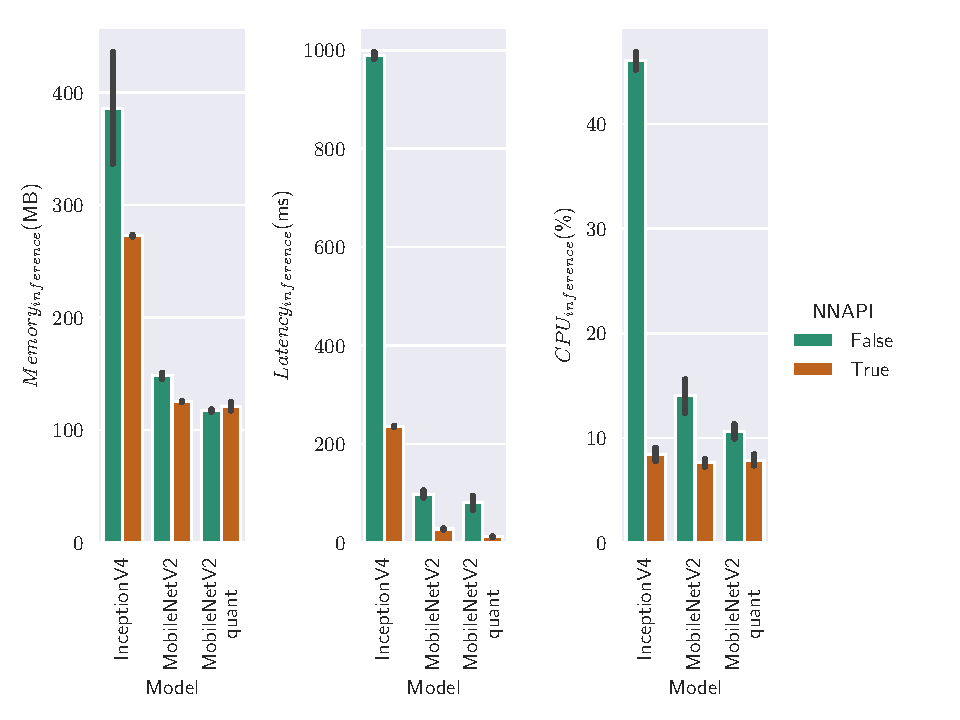
\includegraphics[width=0.9\textwidth]{./Bilder/single_plots/edge_inference_plots/NNAPI_behavior.pdf}
\caption[Edge Inference - Effect of NNAPI on Inference]{Edge Inference - Effect of NNAPI on Inference - lower is better: NNAPI has a significant positive effect on the inference metrics latency, memory and CPU usage.}
\label{fig:NNAPI}
\end{figure}

%, InceptionV4, MobileNetV2 and the quantized version of MobileNetV2,
When comparing the different models with NNAPI enabled it can be stated that there a significant performance differences between these models.
%%MobileNet und Inception vergleichen
%begründen: effect of quant mit paper vergleichen
%unterschiede mobileNet inception vergleichen
%%danahc MobileNet mit quantized
On average, InceptionV4 inference causes higher inference latencies of factor $8$ and consumes twice as much memory as MobileNetV2.
This contrast in performance is as expected, since MobileNetV2 architecture only contains $8\%$ of InceptionV4's parameter number (see table \ref{table:modelOverview}).
This bigger architecture as well as bigger input size lead to higher memory demands and latencies, thus explaining the performance differences.

A similar difference in inference latency can be seen when comparing MobileNetV2 against its quantized version, where the quantized version is more than $2$ times faster, confirming the study results of \cite{Quantizing} presented in section \ref{chap:quant}.
While there is a difference in latency between the quantized and non quantized versions of MobileNetV2, there is no significant discrepancy in memory consumption.



While having big impact on both latency and memory, the different models have 
negligible CPU usage differences, but probably not on GPU usage, which we can not report in this thesis.




%%%%%%%%%%%%%%%%%%%%%%%%%%%%%%%%%%%%%%%%%%%%%%%%%%%%%%%%%%%%%%%%%%%
%%%%%Edge Inference Prepro Vs Inference%%%%%%%%%%%%%%%%%%%%%%%%%%%%%%%%%%

Figure \ref{fig:EdgeInferenceRatio} depicts the latency ratio between preprocessing and inference.
As image sizes increases, the preprocessing becomes more and more the bottleneck, especially for the MobileNetV2 models.
For the MobileNetV2 even $224\times224$ images take longer to preprocess than to perform the inference on them.
%The Inception models are far more computational intensive, hence the longer inference latencies, but still 
\begin{figure}[!htb]
\centering
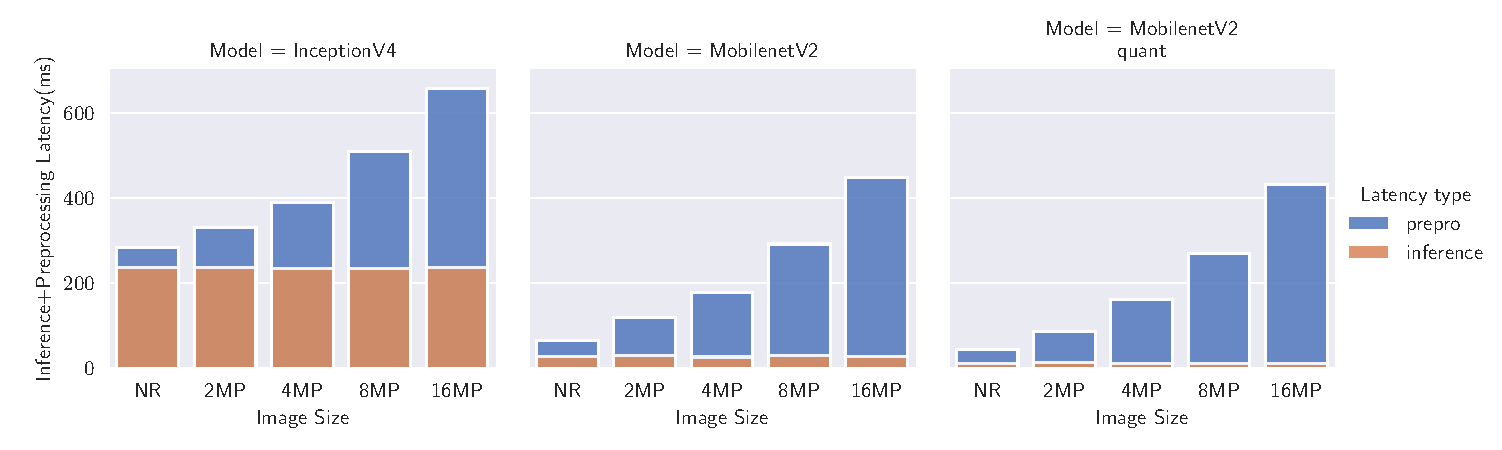
\includegraphics[width=0.95\textwidth]{./Bilder/single_plots/edge_inference_plots/Edge_Preprocessing_+_Inference.pdf}
\caption[Edge Inference - Ratio of Preprocessing and Inference in $Latency_{total}$]{Edge Inference - Ratio of Preprocessing and Inference in $Latency_{total}$ - lower is better: Preprocessing becomes the decisive factor for $Latency_{total}$ of both models for larger image sizes.}
\label{fig:EdgeInferenceRatio}
\end{figure}


\paragraph{Edge Inference - Key Takeaways}
\emph{
\begin{itemize}
    \item Preprocessing becomes bottleneck for larger image sizes.\\
          $16$ MP image in comparison to a $224^2/299^2$ image needs
    \begin{itemize}
        \item $10\times$ slower $Latency_{preprocessing}$
        \item $1.5\times$ more $Memory_{preprocessing}$
    \end{itemize}
    \item NNAPI leads to way better performance across all models:
    \begin{itemize}
        \item $4\times$ faster $Latency_{inference}$
        \item $1.2\times$ less $Memory_{inference}$
        \item $3\times$ less $CPU_{inference}$
    \end{itemize}
    \item In comparison to InceptionV4 MobileNetV2 leads to:
    \begin{itemize}
        \item $8.6\times$ faster $Latency_{inference}$
        \item $2.2\times$ more $Memory_{inference}$
    \end{itemize}
    \item Quantization of MobileNetV2 results in $2.3$x faster $Latency_{inference}$
    \item Preprocessing affects latency more than inference across all images sizes for small networks.
\end{itemize}}

\FloatBarrier
\subsection{Cloud Inference}
This section deals with the results of the cloud inference experiments and their evaluation, divided into preprocessing and inference.
Note that this section only covers the results for a batch size of one, for the results of larger batch sizes please refer to section \ref{chap:resultsBatchSize}.
We are evaluating $Latency_{inference}$ for the most cloud inference results, thus including the network component $Latency_{network}$, because this factor would also be present in real world AI applications. In our case we have a high speed connection with low network latency, thus being a lower bound for real-time AI applications.
%%add network proof (ping and upload)
\subsubsection{Preprocessing}
Cloud Inference allows two preprocessing methods, either on the edge beforehand or directly on the cloud.
This section present the results of these two methods, especially their impact on the resource consumption of edge devices.

Figures \ref{fig:cloudInferencePreproLat} and \ref{fig:cloudInferencePreproMemory} display the effect of preprocessing on either edge or cloud on the preprocessing latencies and memory consumption on the edge in respect to the different deep learning models and image sizes.

For Edge preprocessing, $Memory_{preprocessing}$ and $Latency_{preprocessing}$ are heavily affected by rising image sizes, but not by the different models and their different image input sizes.
Since preprocessing on the edge is very similar as in the edge inference case, please refer to section \ref{chap:edgePrepro} for full details on the edge preprocessing results.

Preprocessing on the cloud leads to an significant decrease in $Latency_{preprocessing}$, which is expected since nearly no preprocessing steps are done on the edge except building a \emph{PredictRequest} object for TensorFlow Serving.
Preprocessing an $224^2/299^2$ image on the edge instead of the cloud causes $20$ times ($1.9/39.8$ms) higher $Latency_{preprocessing}$ and an increase of factor $11$ ($37.9/431.1$ms) for an $16$MP image.
The impact of larger image sizes on memory in the case of cloud preprocessing is marginal, especially in comparison for the edge preprocessing counterparts. This is expected, since only compressed \emph{PNG} images are loaded into memory, in contrary to edge preprocessing, where in addition to the decoded \emph{PNG} images the resized images are also loaded to memory simultaneously.
While $Memory_{preprocessing}$ is lower for cloud preprocessing, the difference is nowhere as substantial as the latency differences. $16$MP images need $1.3$ times ($137.7/179.6$MB) more memory if preprocessing on the edge instead on the cloud.
%%Mention CPU

\begin{figure}[!htb]
\centering
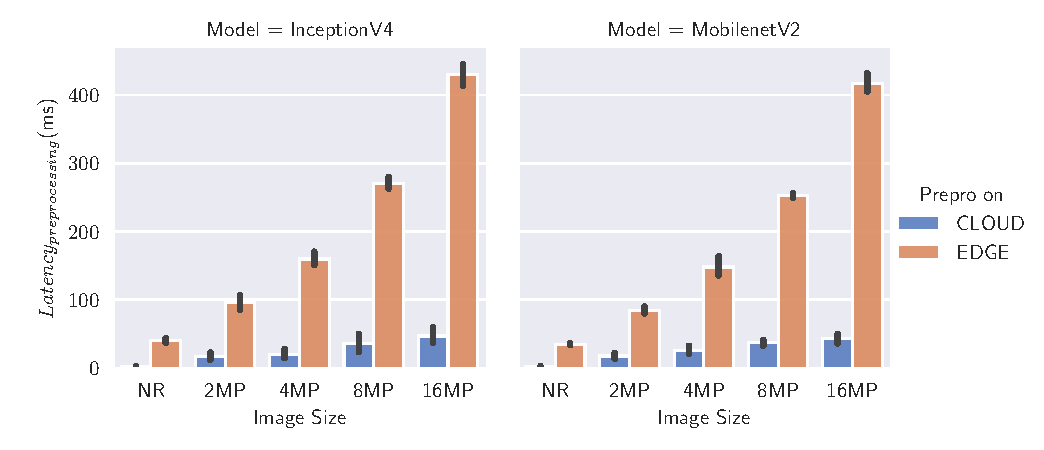
\includegraphics[width=0.95\textwidth]{./Bilder/single_plots/cloud_inference_plots/Cloud_Inference_Preprocessing_Latency.pdf}
\caption{Cloud Inference:  $Latency_{preprocessing}$ - lower is better}
\label{fig:cloudInferencePreproLat}
\end{figure}

\begin{figure}[!htb]
\centering
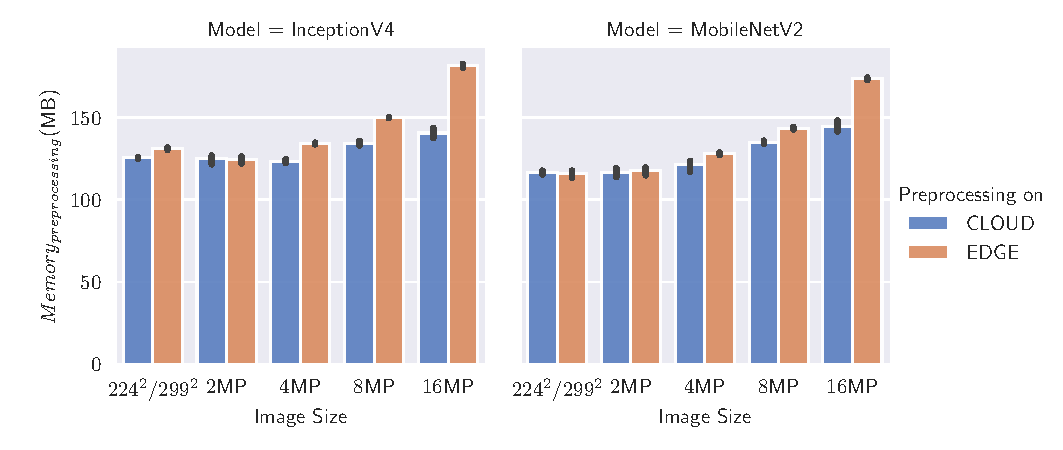
\includegraphics[width=0.95\textwidth]{./Bilder/single_plots/cloud_inference_plots/Cloud_Inference_Preprocessing_Memory.pdf}
\caption{Cloud Inference:  $Memory_{preprocessing}$ - lower is better:}
\label{fig:cloudInferencePreproMemory}
\end{figure}

\FloatBarrier
\subsubsection{Inference}
This section focuses on performance differences between the models and the impact of cloud preprocessing on cloud inference.
The inference metrics for cloud preprocessing include both preprocessing and inference.

%%Also includes preprocessing!!!!

Looking at the memory consumption during inference in figure \ref{fig:cloudInferenceInferenceMemory} one can see that $Memory_{inference}$ is very stable across all image sizes for edge preprocessing, which logical, since all image have been preprocessed to the same shape ($224^2/299^2$), therefore all requests sent to TensorFlow Serving have the same size.
MobileNetV2 uses $10.5$MB less memory on average than InceptionV4, because of its smaller model input size.

For cloud preprocessing the memory consumption increases for increasing image sizes, since larger images are being sent to the server, thus larger images are loaded into the \emph{PredictRequest} object, that is being sent to TensorFlow Serving.
$299^2/224^2$ images consume $123.8/112.34$MB, while $16$MP images $140.1/133.76$, therefore $Memory_{inference}$ increases by $19/13\%$ for InceptionV4/MobileNetV2 respectively.
%%add factor here
There are no $Memory_{inference}$  differences between the two models, since un-preprocessed images are being sent, except for the $224^2/299^2$ images, where the smaller $224^2$ image consumes $7.5$MB less memory on average.
\begin{figure}[!htb]
\centering
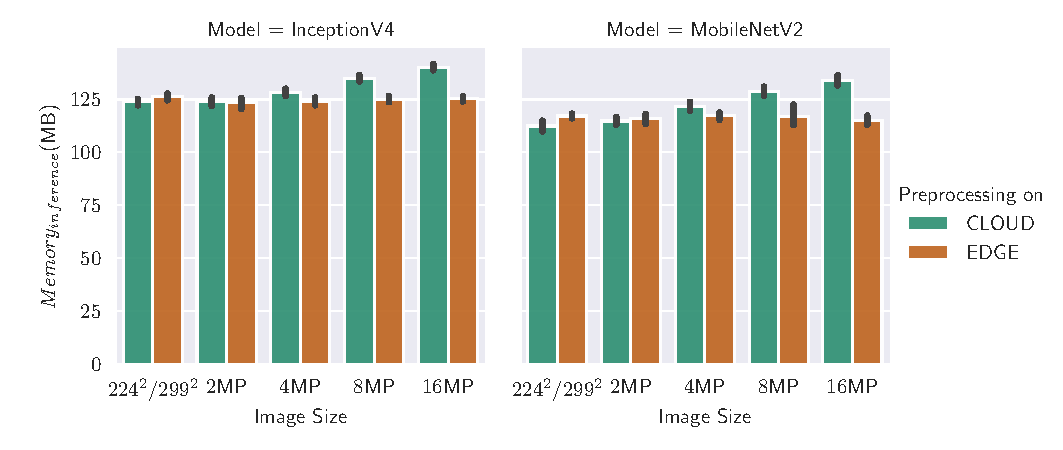
\includegraphics[width=0.95\textwidth]{./Bilder/single_plots/cloud_inference_plots/Cloud_Inference_Memory.pdf}
\caption{Cloud Inference:  $Memory_{inference}$ - lower is better}
\label{fig:cloudInferenceInferenceMemory}
\end{figure}
The $Latency_{inference}$ results can be seen in figure \ref{fig:cloudInferenceInferenceLatency}.
Like for the memory, the latency for edge preprocessing stays the same across all image sizes, since all image sizes are preprocessed on the edge beforehand. 
Mean latencies are $181.2$ms and $108.46$ms for InceptionV4 and MobileNetV2 respectively, therefore MobileNetV2 is $1.7$ times faster.
Figure \ref{fig:CloudInferenceRatioEdgetotal} displays the share of $Latency_{network}$ and $Latency_{server}$ in $Latency_{inference}$ and one can see that the network is accountable for about $20\%$ of the  inference latency for InceptionV4 and $30\%$ for MobileNetV2.

If the images are preprocessed on the cloud, the preprocessing step on the cloud has an significant impact on $Latency_{inference}$, as can be seen in figure \ref{fig:cloudInferenceInferenceLatency}.
While an $224^2/299^2$ image has an latency of $95.8/64.5$ms for InceptionV4/MobileNetV2, a $16$MP image needs $21.9/17.8$ times longer with a $1702.3/1414.8$ms mean latency.
\textbf{This increase applies to all image sizes in a linear proportion.}
Looking at  the share of $Latency_{network}$ in $Latency_{inference}$ in figure \ref{fig:CloudInferenceratioCloudtotal}, the network takes up to $50\%$ of the inference latency for $224^2/299^2$ images, but shrinks to less than $15\%$ for all remaining image sizes.
Therefore it can be stated that the network is not reason for the increase in latency for the larger image sizes, but rather the preprocessing done on the cloud-backend by TensorFlow Serving.
We think Tensorflow's \emph{resize\_bilinear} function, which we use to resize the images, causes the bottleneck in the preprocessing step on the cloud.%%add GPU kernel optimisations issues
%(enter source here)
The use of a other resize approach like nearest-neighbor could speed up preprocessing, but would probably have an impact on the accuracy of the predictions.
While the network connection in our experimentation environment is fast enough too prevent any bottlenecks caused by the network, a slower network connection could slow down inference for large image sizes.
%warum preprocessing s langsam bei tensorflow serving?

%%cloud preprocessing bigger images higher variance
Comparing the two cloud inference options, edge and cloud preprocessing,  $Latency_{inference}$ values for edge preprocessing of both models are faster for all image sizes except the $224^2/299^2$ images.
We believe the $224^2/299^2$ images are faster because of the lower I/O overhead in comparison to the larger preprocessed counter parts, even if the un-preprocessed images still have the decoded and normalized.


This stays also true for $Latency_{total}$ (see figures \ref{fig:CloudInference+PreproCloud} and \ref{fig:CloudInference+PreproEdge}), which includes both $Latency_{preprocessing}$ and $Latency_{inference}$. 
For $224^2/299^2$ images need $223.1/147.2$ms $Latency_{total}$ for InceptionV4/MobileNetV2 for edge preprocessing, while cloud preprocessing needs up $96.9/64.3$ms, therefore cloud preprocessing being $2.3$ times faster.
In contrast cloud inference with edge preprocessing is faster by a factor of $2.7$ for $16$MP images, with the latencies of InceptionV4/MobileNetV2 being $626.7/532$ms for edge preprocessing and $1673.4/1453.9$ms for cloud preprocessing. $2$MP images are $1.7/1.8$ times faster when using edge preprocessing, $4$MP $2.1/2.2$ and $8$MP $2.6/3$ times faster.
%latency edge vs cloud prepro inference:
While MobileNetV2 is $1.75$ times faster in $Latency_{inference}$ for edge preprocessing than InceptionV4, this latency difference shrinks for cloud preprocessing for larger images, started by a difference of factor $1.52$ for $224^2/299^2$ images and shrinking to $1.25/1.21/1.09/1.15$ for the respective image sizes $2/4/8/16$MP.
We believe this decrease is due to the fact as images for MobileNetV2 need to be resized to a smaller input size than InceptionV4, hence increasing the already high resize overhead and thus narrowing the latency difference between both models.
When comparing memory consumption of cloud inference with ether cloud preprocessing or edge preprocessing, the difference is only $3\%$ for  $224^2/299^2$ images ($121.5$MB for edge preprocessing and $118.1$Mb for cloud preprocessing), but $14\%$ for $16$MP images (edge preprocessing $120.0$Mb, cloud preprocessing $136.9$MB).

\begin{figure}[!htb]
\centering
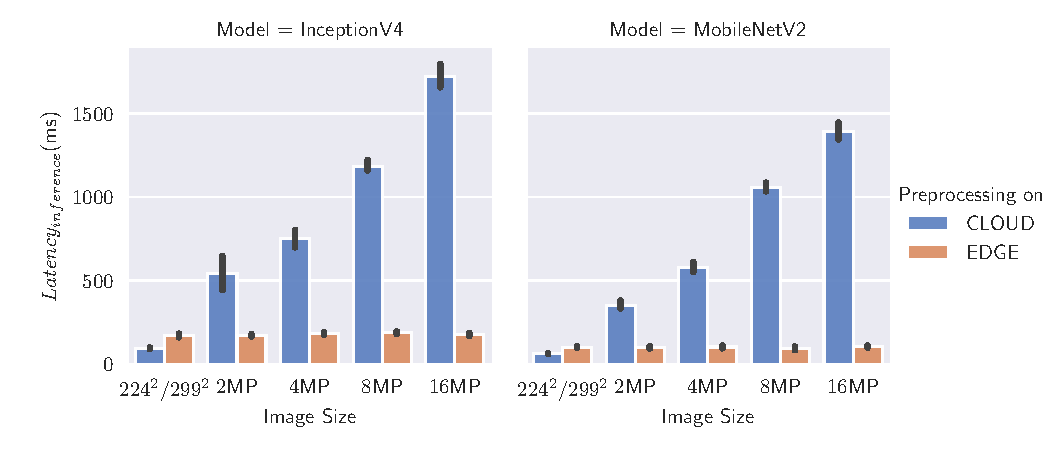
\includegraphics[width=0.95\textwidth]{./Bilder/single_plots/cloud_inference_plots/Cloud_Inference_Latency.pdf}
\caption{Cloud Inference:  $Latency_{inference}$ - lower is better}
\label{fig:cloudInferenceInferenceLatency}
\end{figure}



\begin{figure}[!htb]
\centering
\begin{subfigure}[b]{0.95\textwidth}
   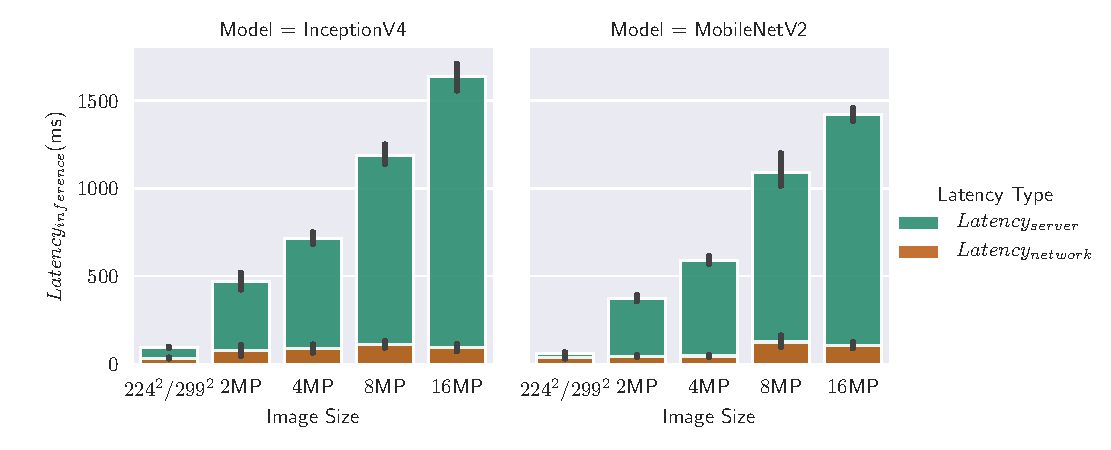
\includegraphics[width=1\linewidth]{./Bilder/single_plots/cloud_inference_plots/Cloud_Server_+_NetworkLatencies_cloudprepro.pdf}
   \caption{Cloud Preprocessing}
   \label{fig:CloudInferenceratioCloudtotal} 
\end{subfigure}

\begin{subfigure}[b]{0.95\textwidth}
   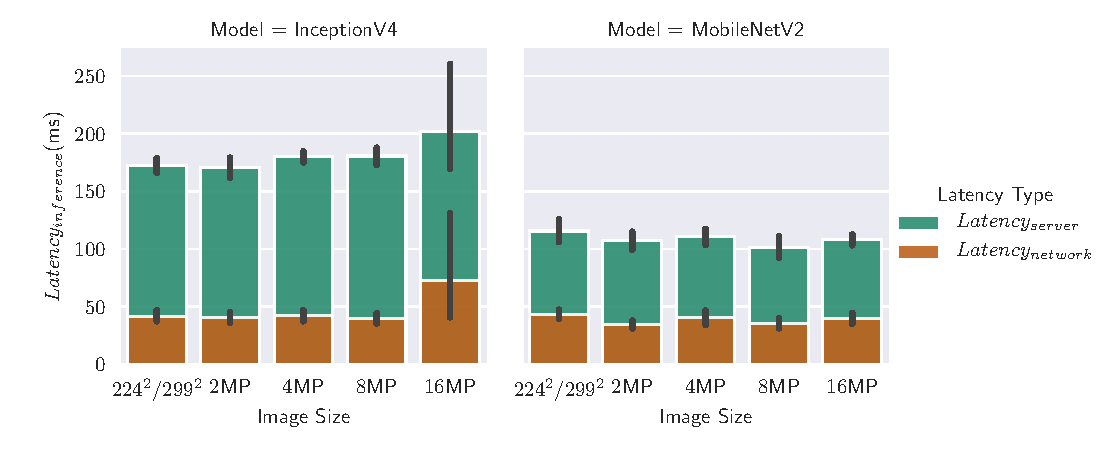
\includegraphics[width=1\linewidth]{./Bilder/single_plots/cloud_inference_plots/Cloud_Server_+_NetworkLatencies_edgeprepro.pdf}
   \caption{Edge Preprocessing}
   \label{fig:CloudInferenceRatioEdgetotal}
\end{subfigure}

\caption{Cloud Inference:  $Latency_{inference}$ including $Latency_{network}$ and $Latency_{server}$ - lower is better}
\end{figure}

\begin{comment}


\begin{figure}[!htb]
\centering
\begin{subfigure}[b]{0.95\textwidth}
   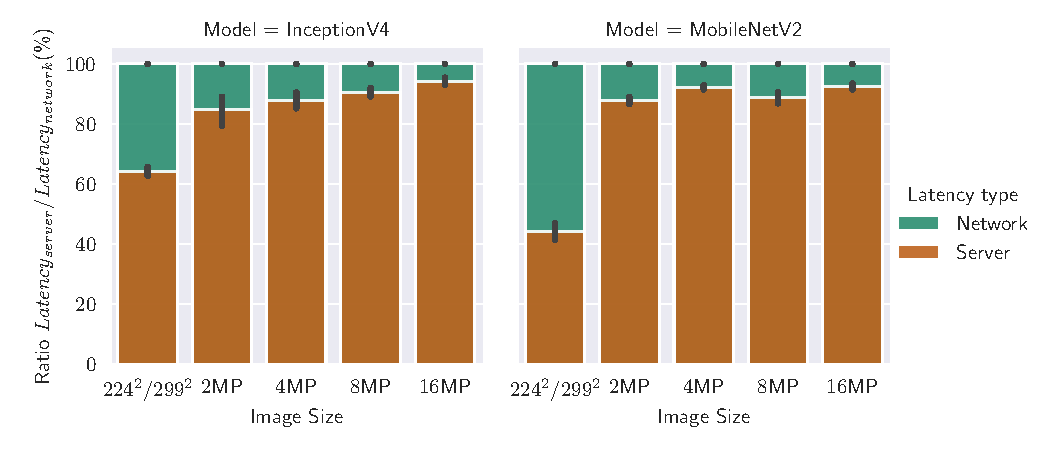
\includegraphics[width=1\linewidth]{./Bilder/single_plots/cloud_inference_plots/Cloud_ratio_server_total_latency_(cloud_prepro).pdf}
   \caption{Cloud Preprocessing}
   \label{fig:CloudInferenceratioCloudrel} 
\end{subfigure}

\begin{subfigure}[b]{0.95\textwidth}
   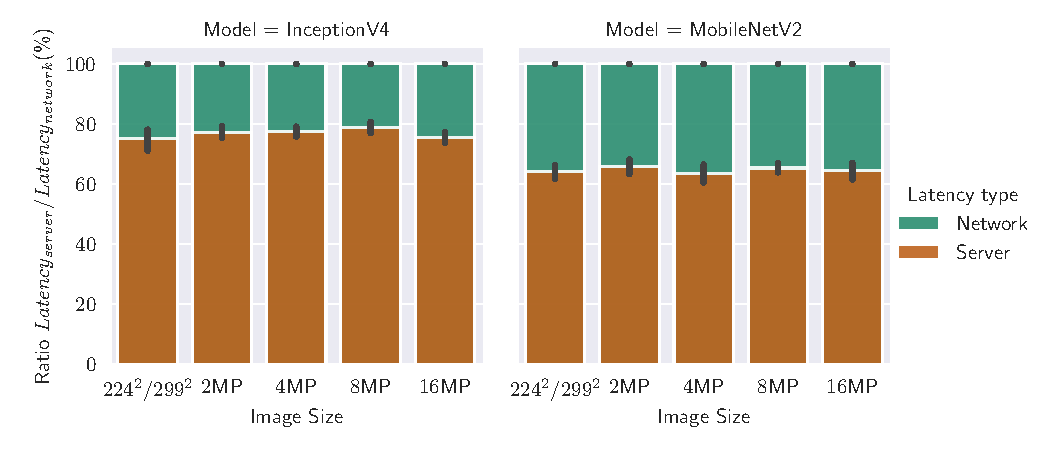
\includegraphics[width=1\linewidth]{./Bilder/single_plots/cloud_inference_plots/Cloud_ratio_server_total_latency_(edge_prepro).pdf}
   \caption{Edge Preprocessing}
   \label{fig:CloudInferenceRatioEdgerel}
\end{subfigure}

\caption{Cloud Inference:  Ratio between $Latency_{network}$ and $Latency_{server}$ - lower is better}
\end{figure}
\end{comment}


\begin{figure}[!htb]
\centering
\begin{subfigure}[b]{0.95\textwidth}
   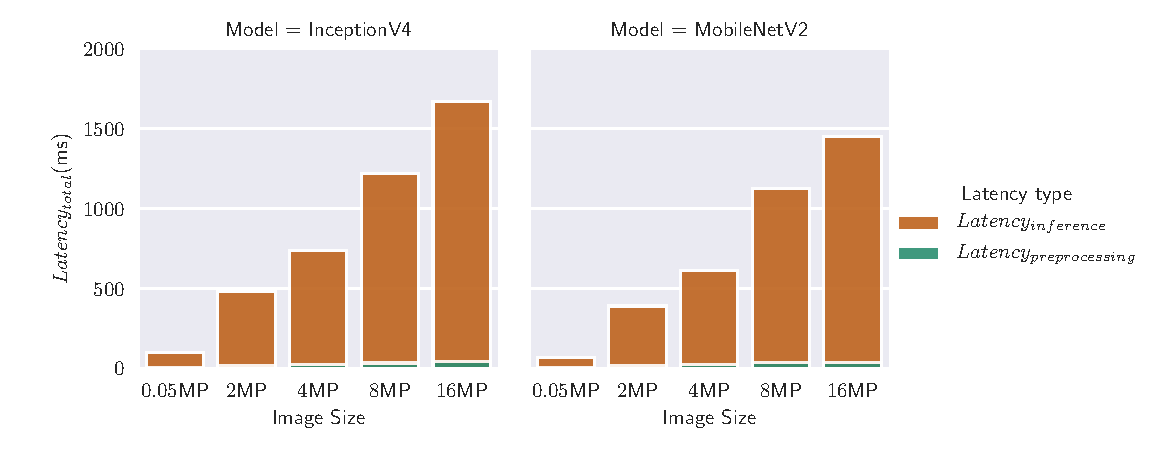
\includegraphics[width=1\linewidth]{./Bilder/single_plots/cloud_inference_plots/Cloud_Preprocessing_Inference_Comb_cloud_prepro.pdf}
   \caption{Cloud Preprocessing}
   \label{fig:CloudInference+PreproCloud} 
\end{subfigure}

\begin{subfigure}[b]{0.95\textwidth}
   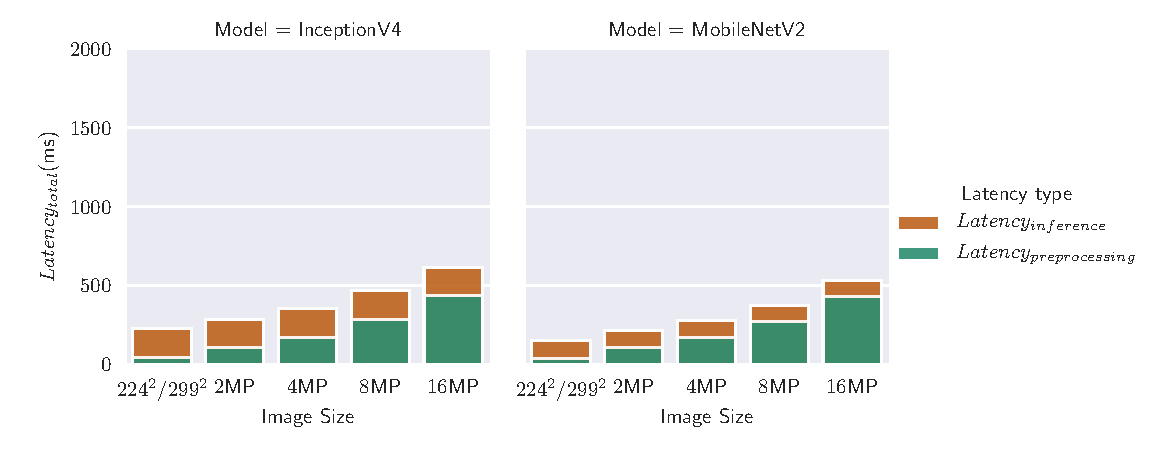
\includegraphics[width=1\linewidth]{./Bilder/single_plots/cloud_inference_plots/Cloud_Preprocessing_Inference_Comb_edge_prepro.pdf}
   \caption{Edge Preprocessing}
   \label{fig:CloudInference+PreproEdge}
\end{subfigure}

\caption{Cloud Inference:  $Latency_{preprocessing}$ and $Latency_{inference}$ combined - lower is better}
\end{figure}

Figures \ref{fig:CloudInferenceReceivedData} and \ref{fig:CloudInferenceTransmittedData} show the data transmitted and received from the edge client to the cloud-backend server for the different image sizes and preprocessing options.
For edge processed image the mean transmitted data is $1061.9/608.7$KB for InceptionV4/MobileNetV2 and $16.7/10.3$KB data received by the respective models.
Therefore $299^2$ images require $453.2$ kilobytes more than $224^2$ images.
For cloud preprocessing $Data_{transmitted}$ the amount of data sent is at maximum $100$KB larger than the sizes of the \emph{PNG} images ($224^2$: $83$KB, $299^2$: $141$KB, $2$MP: $2411$KB, $4$MP: $4309$KB, $8$MP: $7515$KB,  $16$MP: $10077$KB).
For both edge and cloud preprocessing the $Data_{received}$ rises for rising $Data_{transmitted}$ values, since the communication between server and client is done via TCP, thus more sent data results in more packages resulting in more ACK signals getting sent back to the client.
%%NR:[114.5] transmitted
%%NR:[3.] received
%%2MP:[2446.2] transmitted
%%2MP:[38.2] received
%%4MP:[4365.5] transmitted
%%4MP:[64.8] received
%%8MP:[7603.6] transmitted
%%8MP:[114.9] received
%%16MP:[10176.8] transmitted
%%16MP:[141.4] received
%299 png kleiner als 299 preporcessing
%%mit echter bildgröße abgleichen
%2MP($1732\times1155$, $2411$KB), 4MP($2449\times1633$, $4309$KB), 8MP($3464\times2309$, $7515$KB) and 16MP($4899\times3266$, $10077$KB) ($224\times224$, $83$KB or $299\times299$, $141$KB


\begin{figure}[!htb]
\centering
\begin{subfigure}[b]{0.95\textwidth}
   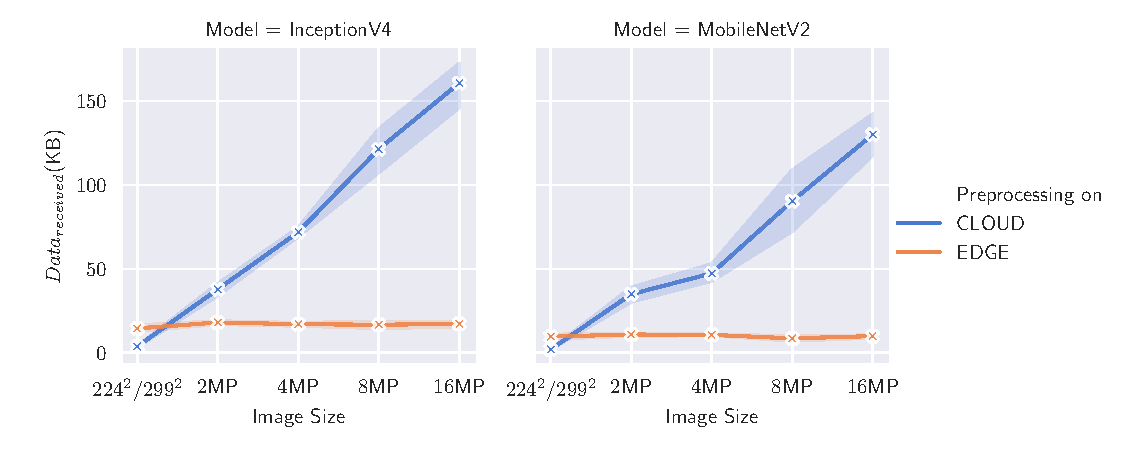
\includegraphics[width=1\linewidth]{./Bilder/single_plots/cloud_inference_plots/Cloud_Inference_Received_Data.pdf}
   \caption{$Data_{received}$}
   \label{fig:CloudInferenceReceivedData} 
\end{subfigure}

\begin{subfigure}[b]{0.95\textwidth}
   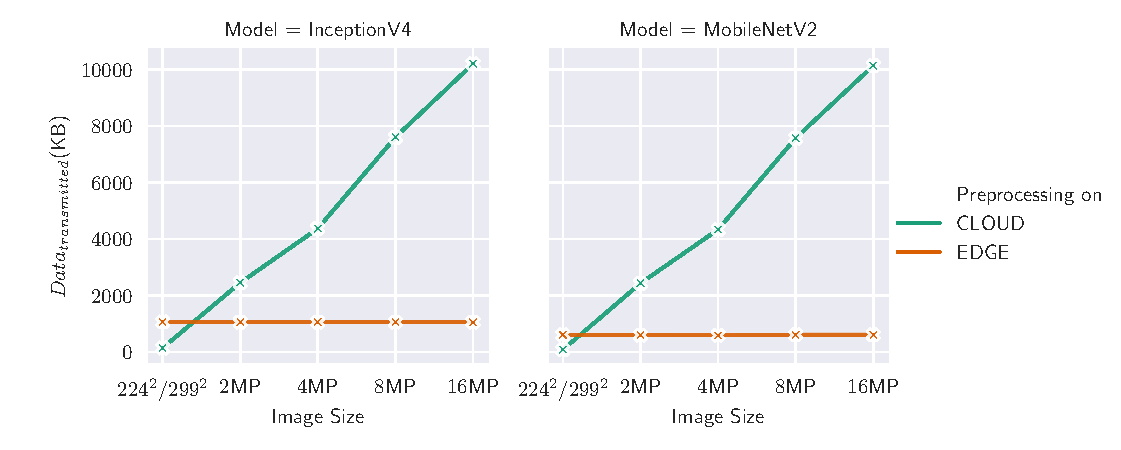
\includegraphics[width=1\linewidth]{./Bilder/single_plots/cloud_inference_plots/Cloud_Inference_Transmitted_Data.pdf}
   \caption{$Data_{transmitted}$}
   \label{fig:CloudInferenceTransmittedData}
\end{subfigure}

\caption{Cloud Inference:  $Data_{received}$ vs. $Data_{transmitted}$ - lower is better}
\end{figure}

\FloatBarrier
\paragraph{Cloud Inference - Key Takeaways}
%cloud prepro less preprocessing memory and latency
%cloud prepro more inference memory
%cloud preprocessing very slow for large image sizes
%edge prepro faster for all image sizes except 224/299
%network not a bottlneck
%resize binlinear bad implementation?
\emph{
\begin{itemize}
    \item Preprocessing on the cloud in comparison to edge preprocessing causes:
    \begin{itemize}
        \item $20\times$ faster $Latency_{preprocessing}$ for $224^2/299^2$ images
        \item $10\times$ faster $Latency_{preprocessing}$ for $16$MP images
        \item $1.28\times$ less $Memory_{preprocessing}$ for $16$MP images
    \end{itemize}
    \item Inference on the cloud including preprocessing in comparison to cloud inference without preprocessing causes:
    \begin{itemize}
        \item $2.3\times$ faster InceptionV4/MobileNetV2 $Latency_{total}$ for $224^2/299^2$ images
        \item $2.7\times$ slower InceptionV4/MobileNetV2 $Latency_{total}$ for $16$MP images
        \item $0.97\times$ less $Memory_{inference}$ for $224^2/299^2$ images
        \item $1.14\times$ more $Memory_{inference}$ for $16$MP images
    \end{itemize}
    \item MobileNetV2 is up to $1.75\times$ faster than InceptionV4 for smaller images, but shrinking to around $10\%$ faster for large image in case of cloud preprocessing.
    \item Network is accountable for up to $50\%$ of $Latency_{inference}$ for $224^2/299^2$ images and networks, but less than $30\%$ for larger images and network for both cloud and edge preprocessing.
\end{itemize}
\begin{itemize}[leftmargin=4em]
 \renewcommand{\labelitemi}{$\Rightarrow$}
 \item Edge Preprocessing has faster $Latency_{total}$ latencies for all image sizes except $224^2/299^2$.
\end{itemize}
}%emph end


\subsection{Edge vs. Cloud Inference}
Previous two sections presented the results for both edge and cloud inference.
Now, the results of the cloud and the edge inference with batch size one, including preprocessing, are compared against each other.
First preprocessing and inference are evaluated separately and afterwards both of the steps combined. 
Each plot of this section contains five subplots, one for each image sizes, the x-axis contains the deep learning model, while the y-axis displays the various performance metrics. 
The legend used in all those plots in explained in table \ref{table:legendPlots}.
\begin{table}[!htb]
\newcommand\crule[3][black]{\textcolor{#1}{\rule{#2}{#3}}}
\centering
\caption{Explanation of the plot legends}
\label{table:legendPlots}
\begin{tabular}{@{}lll@{}}
\toprule
Inference on & Description & Color \\ \midrule
\begin{tabular}[c]{@{}l@{}}Inf on:CLOUD;\\ Prepro on:CLOUD\end{tabular} & \begin{tabular}[c]{@{}l@{}}Inference as well as preprocessing is done on the\\ cloud-backend.\end{tabular} &  \crule[gruen]{0.8cm}{0.8cm}\\
\begin{tabular}[c]{@{}l@{}}Inf on:CLOUD;\\ Prepro on:EDGE\end{tabular} & \begin{tabular}[c]{@{}l@{}}Inference is done on cloud-backend, but images are \\ preprocessed on edge beforehand.\end{tabular} &  \crule[orangedunkel]{0.8cm}{0.8cm}\\
\begin{tabular}[c]{@{}l@{}}Inf on:EDGE;\\ Prepro on:EDGE\end{tabular} & \begin{tabular}[c]{@{}l@{}}Inference as well as preprocessing is done on the\\ edge.\end{tabular} & \crule[lila]{0.8cm}{0.8cm} \\ \bottomrule
\end{tabular}
\end{table}

Not that for the quantized MobileNetV2 we only conduct edge inference experiments, thus no cloud inference results for this model can be seen in the plots of this section.
\subsubsection{Preprocessing}

Figures \ref{fig:EdgeVsCloudPreproMemory}, \ref{fig:EdgeVsCloudPreproLat} and \ref{fig:CloudEdgePreproCPU} report the preprocessing metrics $Memory_{preprocessing}$, $Latency_{preprocessing}$ and $CPU_{preprocessing}$.

%Memory
\paragraph{$\mathbf{Memory_{preprocessing}}$}
Both edge preprocessing options, for either edge inference or cloud inference, have very similar memory consumption results with the cloud inference mean values being at most $5.5\%$ higher from the edge inference values for all image sizes.
This due to the fact that both options share most of the preprocessing steps, the only difference is that in case of cloud inference with edge preprocessing the \emph{ByteBuffer}, containing the preprocessed image, gets used to build the \emph{PredictRequest} for TensorFlow Serving. 
For edge inference no such step is needed as the \emph{ByteBuffer} can be directly be used to call the run function of the TensorFlow Lite interpreter, which starts the inference process at the edge.
Thus the $5.5\%$ overhead in memory can be explained by the additional \emph{PredictRequest} object that has to loaded into memory for cloud inference.

In case of small images the memory consumption of cloud preprocessing is very close to its edge preprocessing counter-part, the larger the image the larger the memory difference.
While the difference is only $1.9\%$ for an $224^2/299^2$ image ($114.53/116.69$MB), the difference grows to an $22.5\%$ decrease ($177.8/137.8$MB)in memory for $16$MP images ($2$MP: $1.1\%$, $4$MP: $7.9\%$, $8$MP: $9.9\%$).
This difference is caused by the fact that for cloud preprocessing only the compressed \emph{PNG} gets loaded into memory, which is a lot smaller than the decoded image, especially for large images such as the $16$MP image.

When comparing the different models InceptionV4 ($140.1$MB) consumed about $7.9$MB more $Memory_{preprocessing}$ than MobileNetV2 ($132.2$MB), or about $6\%$, independent of image size or inference mode (edge inference, cloud inference with edge preprocessing and cloud inference with cloud preprocessing).
Edge inference of the quantized version of MobileNetV2 causes the same memory consumption as the non quantized version.
When differentiating between the different image sizes and inference modes the difference is always between $4-8\%$, except for cloud preprocessing of an $224^2/299^2$ image, where the difference rises to $10\%$ ($11.35$MB). This is due to the fact that MobileNetV2 preprocesses $224^2$ images and InceptionV4 $299^2$ images.

%Latency
\paragraph{$\mathbf{Latency_{preprocessing}}$}
The preprocessing latency results are similar to the memory results. Both edge preprocessing options are very similar in performance, while cloud preprocessing performs better, but in case of latency the difference is larger.

The difference between the edge preprocessing options (cloud inference with edge preprocessing and edge preprocessing) is at most $4.9\%$ ($5.1$ms) across all images sizes (not differentiating between the different models).

When comparing edge preprocessing to cloud preprocessing the latency gap for $224^2/299^2$ images is a factor of $20$ in the favor of cloud preprocessing ($1.9/38.2$ms). For larger image sizes this gap shrinks, but still amounts $11\times$ for $16$MP images ($37.9/430.78$ms).

The different models have little to no impact on the preprocessing when comparing same images sizes.
For cloud preprocessing the MobileNetV2 and InceptionV4 differ at most $4.9$ms (for $8$MP, all other image size are below that for both relative and total difference). This difference is not significant since the standard deviation for the mean values is more than twice as high for both models.
%%difference between models for edge preporcessing
%%%model compare
%cloud prepro no diff for models
%%diff for NR large for edge prepro -> normalizing more work
This is also true for edge preprocessing for all image sizes, regardless of edge or cloud inference.
Although the difference between the models is up to $29\%$ or $10.3$ms ($224^2/299^2$ image), the speedup is not significant as the standard deviation for both models is above $9$ms.

%CPU
\paragraph{$\mathbf{CPU_{preprocessing}}$}
Looking at the CPU usages in figure \ref{fig:CloudEdgePreproCPU} it can be seen that the variance of all inference modes, models and images sizes is too large to make conclusions, although there is a indication that cloud preprocessing causes lower usages.
Overall it can be stated that all usages are around $12.5\%$. This makes sense since the preprocessing of a single image is done on a single thread, thus running on one core and since the OnePlus 6T has 8 cores, the full utilization of a single core causes an overall $CPU_{preprocessing}$  usage of $12.5\%$. 
This infers that the preprocessing uses $100\%$ of a single core, especially for large images.

\begin{figure}[!htb]
\centering
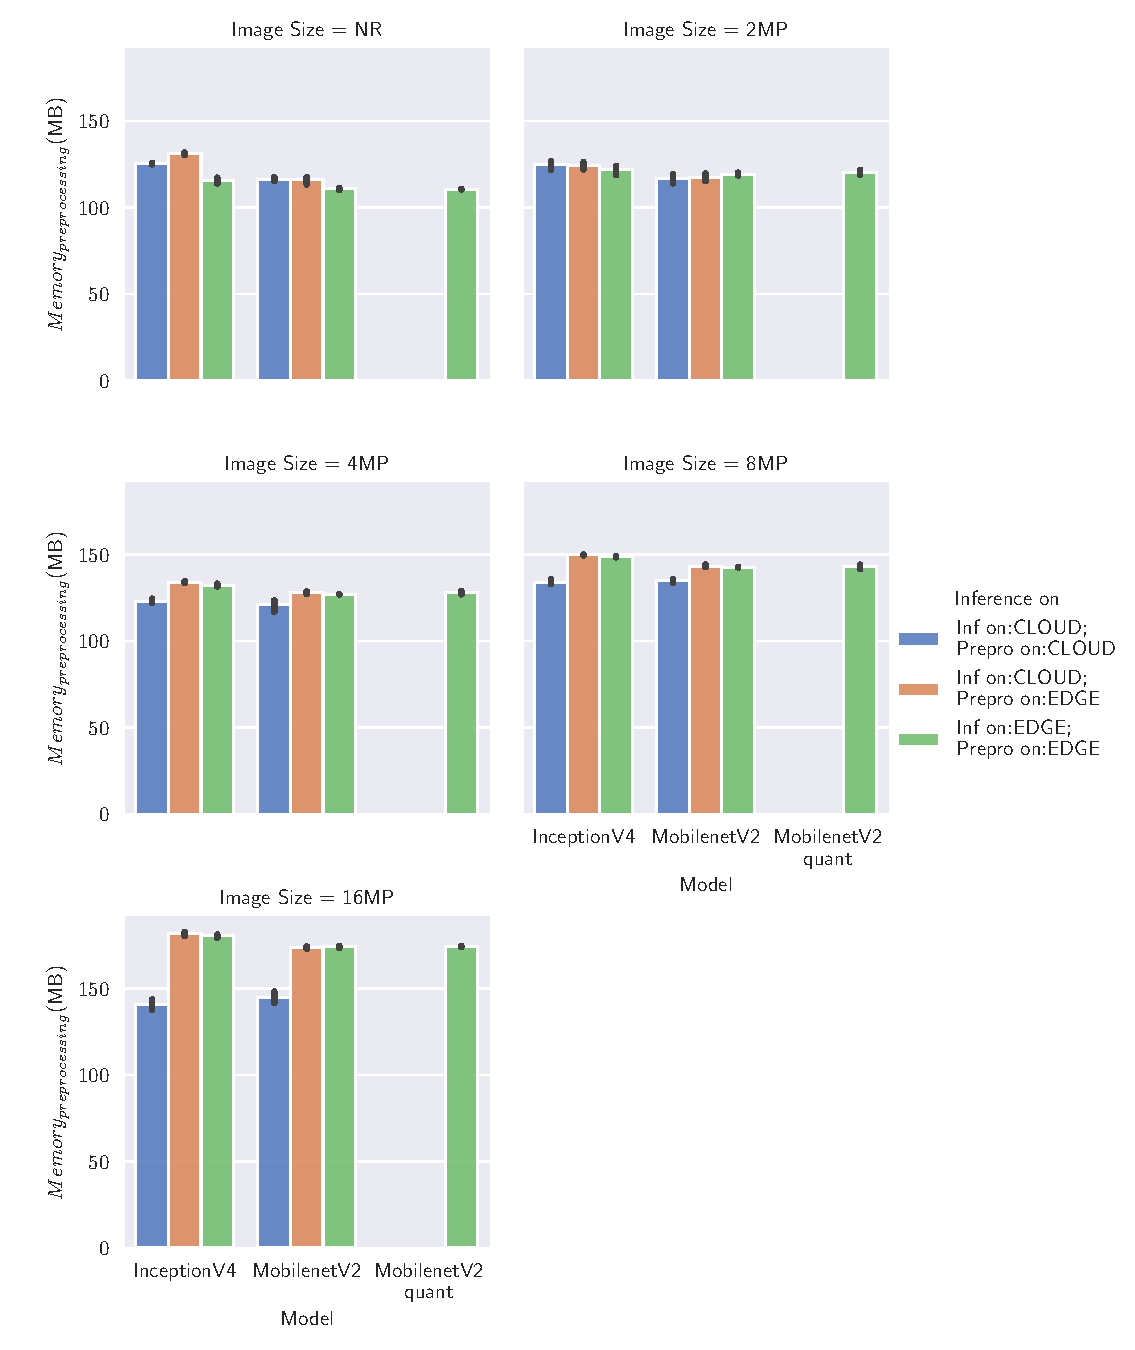
\includegraphics[width=0.95\textwidth]{./Bilder/single_plots/edge_vs_cloud_plots/Edge_vs_Cloud_Inference_Preprocessing_Memory.pdf}
\caption{Edge vs. Cloud Inference:  $Memory_{preprocessing}$ - lower is better}
\label{fig:EdgeVsCloudPreproMemory}
\end{figure}

\begin{figure}[!htb]
\centering
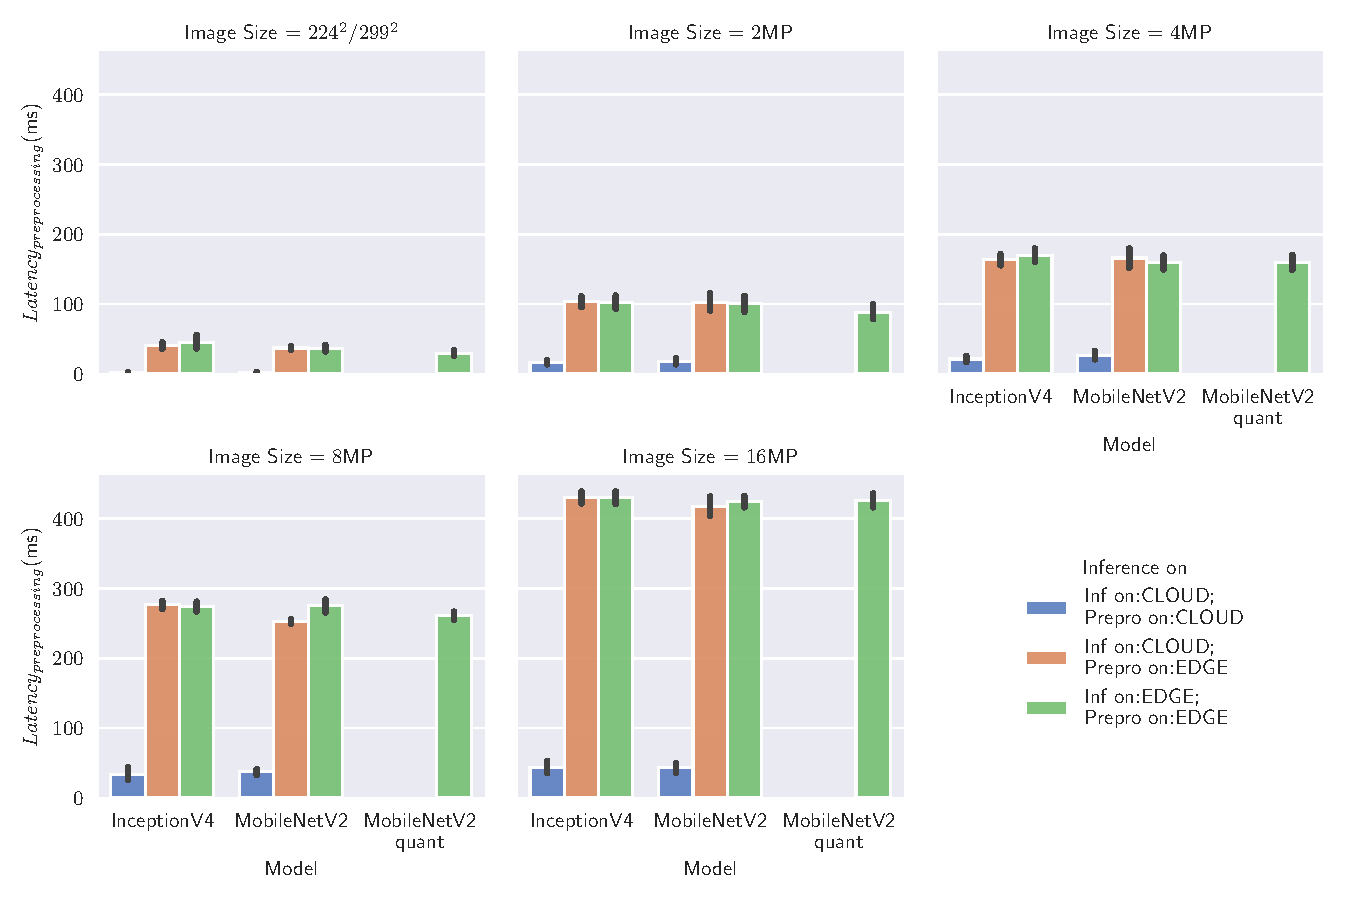
\includegraphics[width=0.95\textwidth]{./Bilder/single_plots/edge_vs_cloud_plots/Edge_vs_Cloud_Inference_Preprocessing_Latencies.pdf}
\caption{Edge vs. Cloud Inference:  $Latency_{preprocessing}$ - lower is better}
\label{fig:EdgeVsCloudPreproLat}
\end{figure}

\FloatBarrier
\subsubsection{Inference}
\paragraph{$\mathbf{Memory_{inference}}$}
Figure \ref{fig:EdgeVsCloudInferenceMemory} reports $Memory_{inference}$ for all inference modes, models and image sizes.
Image size has no impact on the memory consumption during inference, where image have been previously preprocessed, which is logical, since the preprocessed image have the same memory constraints regardless of the size before preprocessing.
In contrary cloud inference with cloud preprocessing memory consumption is impacted by different image sizes, since the images are not preprocessed and thus larger images are being sent to the server.
$16$MP images use $19\%$ more memory for InceptionV4 in comparison to a $224^2/299^2$ image and $13\%$ more for MobileNetV2.


While different images sizes only have a small impact on $Memory_{inference}$ different inference modes (edge inference, cloud inference with either edge or cloud preprocessing) do have a large impact, especially in the case of the large InceptionV4 network.
Edge Inference with InceptionV4 consumes more than twice ($2.2\times$) as much memory than both cloud inference options.

While cloud inference for InceptionV4 can half memory consumption, MobileNetV2 does not profit nearly as much from cloud inference, as edge inference with MobileNetV2 only uses $10.5\%$ ($13.6$MB) more an average (independent of image size) than cloud inference with edge preprocessing due to its small model size.
Edge inference with MobileNetV2 uses less memory than cloud inference with cloud preprocessing for $16$MP images, as the un-preprocessed image consumes more memory than the loaded model. 

The quantization of MobileNetV2 has no significant impact on memory consumption.


%inception on egde much more, mobilenet nearly equal (more for small images, less forlarge images than cloud prepro)
\paragraph{$\mathbf{Latency_{inference}}$}
Results for $Latency_{inference}$ can be seen in figures \ref{fig:EdgeVsCloudInferenceLat} and \ref{fig:EdgeVsCloudInferenceLatNR}, while the latter only contains the latency results for the $224^2/299^2$ size for better readability and the first one for all images sizes.
These figures show the substantial difference in latency between the different deployment options, models and image sizes.
Recall that the cloud inference results include the network latency $Latency_{network}$, because this factor would also be present in real world AI applications.  In our case we have a high speed connection with low network latency, thus being a lower bound for real-time AI applications.

For InceptionV4 and $224^2/299^2$ images cloud inference with cloud preprocessing is the fastest inference method with a mean of $94.9$ms, followed by cloud inference with edge inference ($180.4$ms) and cloud inference with edge preprocessing ($235.9$ms).
We believe this difference between the two cloud inference options is due to lower I/O overhead as well as smaller network latency in case of cloud preprocessing, since the compressed $224^2/299^2$ \emph{PNG} images are smaller in size than the decoded counter-parts. 
In contrary in the case of MobileNetV2 edge inference is the fastest option for $224^2/299^2$ images with a mean of $27.7$ms, followed by cloud inference with cloud preprocessing ($62.5$ms) and lastly cloud inference with edge preprocessing ($110.2$ms).
When neglecting the $Latency_{network}$ part in $Latency_{inference}$, cloud inference with cloud preprocessing is nearly as fast as edge inference with MobileNetV2 with a difference of $0.26$ms.

Therefore the fastest $224^2/299^2$ image option for MobileNetV2 is the edge inference option, while for InceptionV4 cloud inference is the optimal choice.

The quantized version of MobileNetV2 has a mean inference latency of $11.7$ms, thus being $1.9$ times faster than edge inference of non quantized MobileNetV2 and $8.1$ times faster than the best InceptionV4 result.

While the various images sizes have no impact on inference methods, where images have been previously preprocessing on the edge, they have severe impact on cloud inference with cloud preprocessing.
With the average latencies for InceptionV4/MobileNetV2 for an $16$MP images being $1633.9/1417.6$ms, the difference to a $224^2/299^2$ image is more than factor $17/22$.
%%standard deviation larger for cloud preprocessing of large images

\paragraph{$\mathbf{CPU_{inference}}$}
%not interesting
Figure \ref{fig:EdgeVsCloudInferenceCPU} shows that there are no severe differences in CPU usage between edge and cloud inference, regardless of model and image size, at least for the case of batch size of one.
All usages are below $12.5\%$, therefore no core is utilized fully, since the OnePlus 6T used in our experiments has $8$ cores.


\paragraph{$\mathbf{Throughput_{inference}}$}
Since $Throughput_{inference}$ is directly computed from $Latency_{inference}$, the results for this metric in figure \ref{fig:EdgeVsCloudinferneceThroughput} have the same tendencies as the latencies.
Hence cloud inference with cloud preprocessing is the best inference option for InceptionV4, at least in the case of $224^2/299^2$ images with a mean throughput of $10.8$ predictions per second.
Meanwhile for MobileNetV2 reaches up to $36.6$ predictions per second, when inference is done at the edge.
The quantized version of MobileNetV2 can make up to $83.7$ predictions per second.

While $Throughput_{inference}$ stays constant across all images sizes for edge preprocessing options, cloud inference with cloud preprocessing is impacted severely with a drop to $0.6$ predictions per second for the case of InceptionV4, $16$MP.


\paragraph{$\mathbf{Throughput_{total}}$}
So far we only evaluated the results of preprocessing and inference separately, but especially for the metrics throughput and latency the sum of both preprocessing and inference is of interest.%,since 
When looking at the $Throughput_{total}$, which is derived from the sum of $Latency_{preprocessing}$ and $Latency_{inference}$ in figure \ref{fig:EdgeVsCloudTotalThroughput} the impact of preprocessing on the throughput can be seen.
While this impact is small for cloud inference with cloud preprocessing, because $Latency_{preprocessing}$ values for this option are very small, the impact is significant for inference methods with edge preprocessing.
But even when accounting for both preprocessing and inference, cloud inference with cloud preprocessing performs way worse for large image sizes than both edge preprocessing methods.

First we evaluate the results for the $224^2/299^2$ images.
When including preprocessing  the throughput of MobileNetV2 on the edge drops from $36.6$ to $16.1$, since preprocessing takes longer than the actual inference, even for a image where no resizing has to be done.
which is very close to the best cloud inference option for this model ($15.7$)

For the quantized version of MobileNetV2 the preprocessing latency is the same as for the non quantized counter-part, but the lower inference latency leads to a total throughput of $23.1$.

When analyzing the larger images sizes preprocessing takes a significant toll on all deployment options, as throughput of MobileNetV2/InceptionV4 drops to $7.8/3.6$, $5.3/2.8$, $3.3/2.2$, $2.1/1.6$ for the image sizes $2$MP, $4$MP, $8$MP and $16$MP respectively (reporting the values for the best inference option for each image size).
Even tough cloud inference with preprocessing has the lowest preprocessing latency, the remain the worst inference option except for the $224^2/299^2$ images.

\begin{figure}[!htb]
\centering
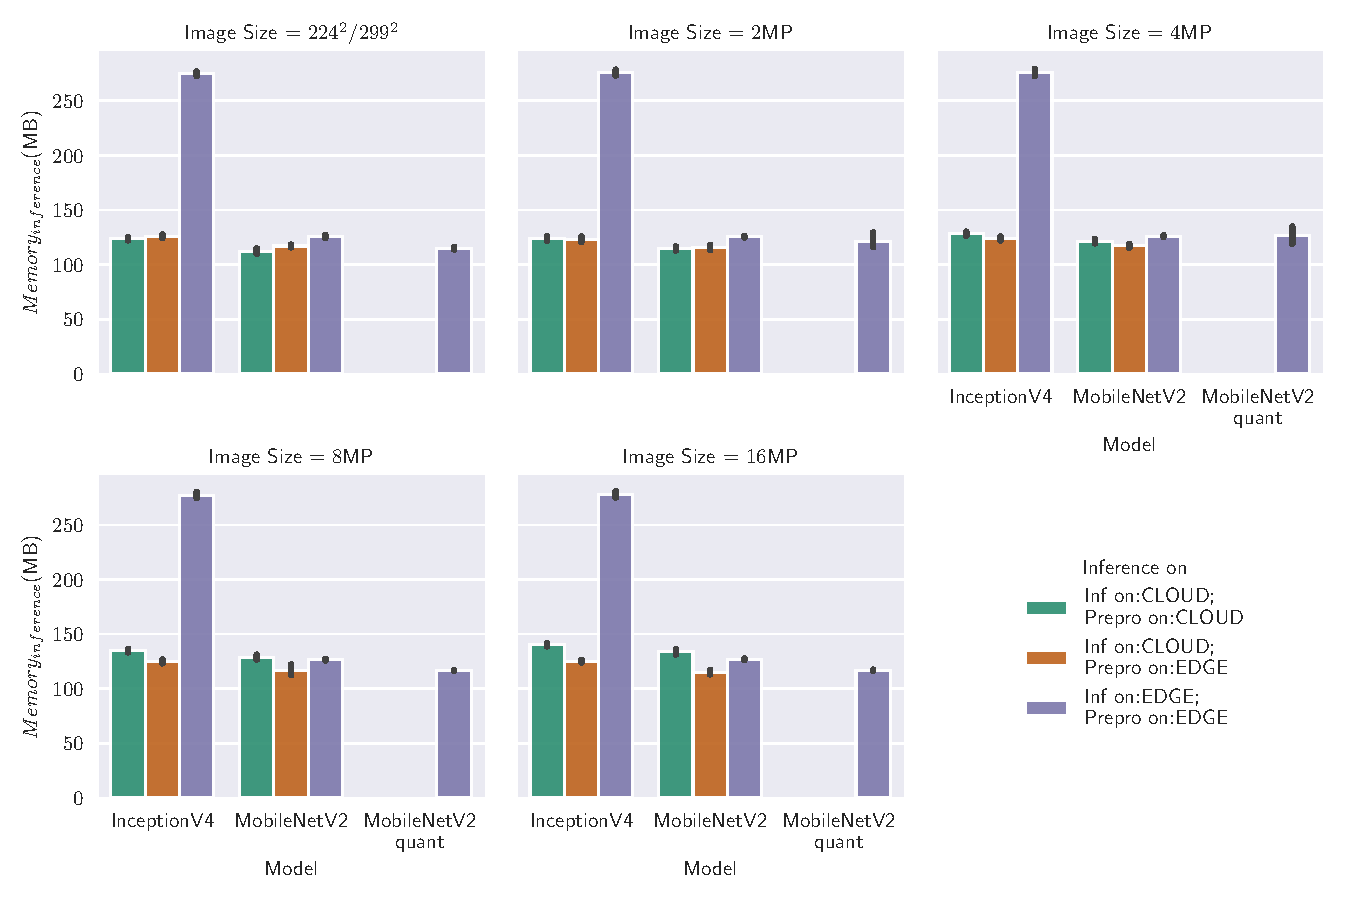
\includegraphics[width=0.95\textwidth]{./Bilder/single_plots/edge_vs_cloud_plots/Edge_vs_Cloud_Inference_Inference_Memory.pdf}
\caption[{Edge vs. Cloud Inference:  $Memory_{inference}$ - lower is better}]{Edge vs. Cloud Inference:  $Memory_{inference}$ - lower is better - InceptionV4 has significant impact on memory consumption in case of edge inference, while MobileNetV2 small size has very little impact.}
\label{fig:EdgeVsCloudInferenceMemory}
\end{figure}

\begin{figure}[!htb]
\centering
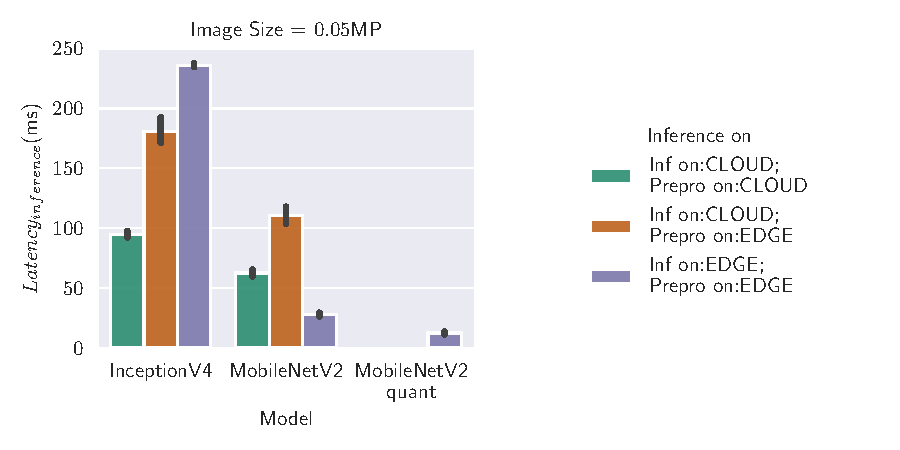
\includegraphics[width=0.95\textwidth]{./Bilder/single_plots/edge_vs_cloud_plots/Edge_vs_Cloud_Inference_Inference_Latencies_onlyNR.pdf}
\caption[Edge vs. Cloud Inference:  $Latency_{inference}$ of $224^2/299^2$ images - lower is better]{Edge vs. Cloud Inference:  $Latency_{inference}$ of $224^2/299^2$ images - lower is better - For InceptionV4 cloud inference is the fastest option, while for MobileNetV2 edge inference is the preferred option.}
\label{fig:EdgeVsCloudInferenceLatNR}
\end{figure}
\begin{figure}[!htb]
\centering
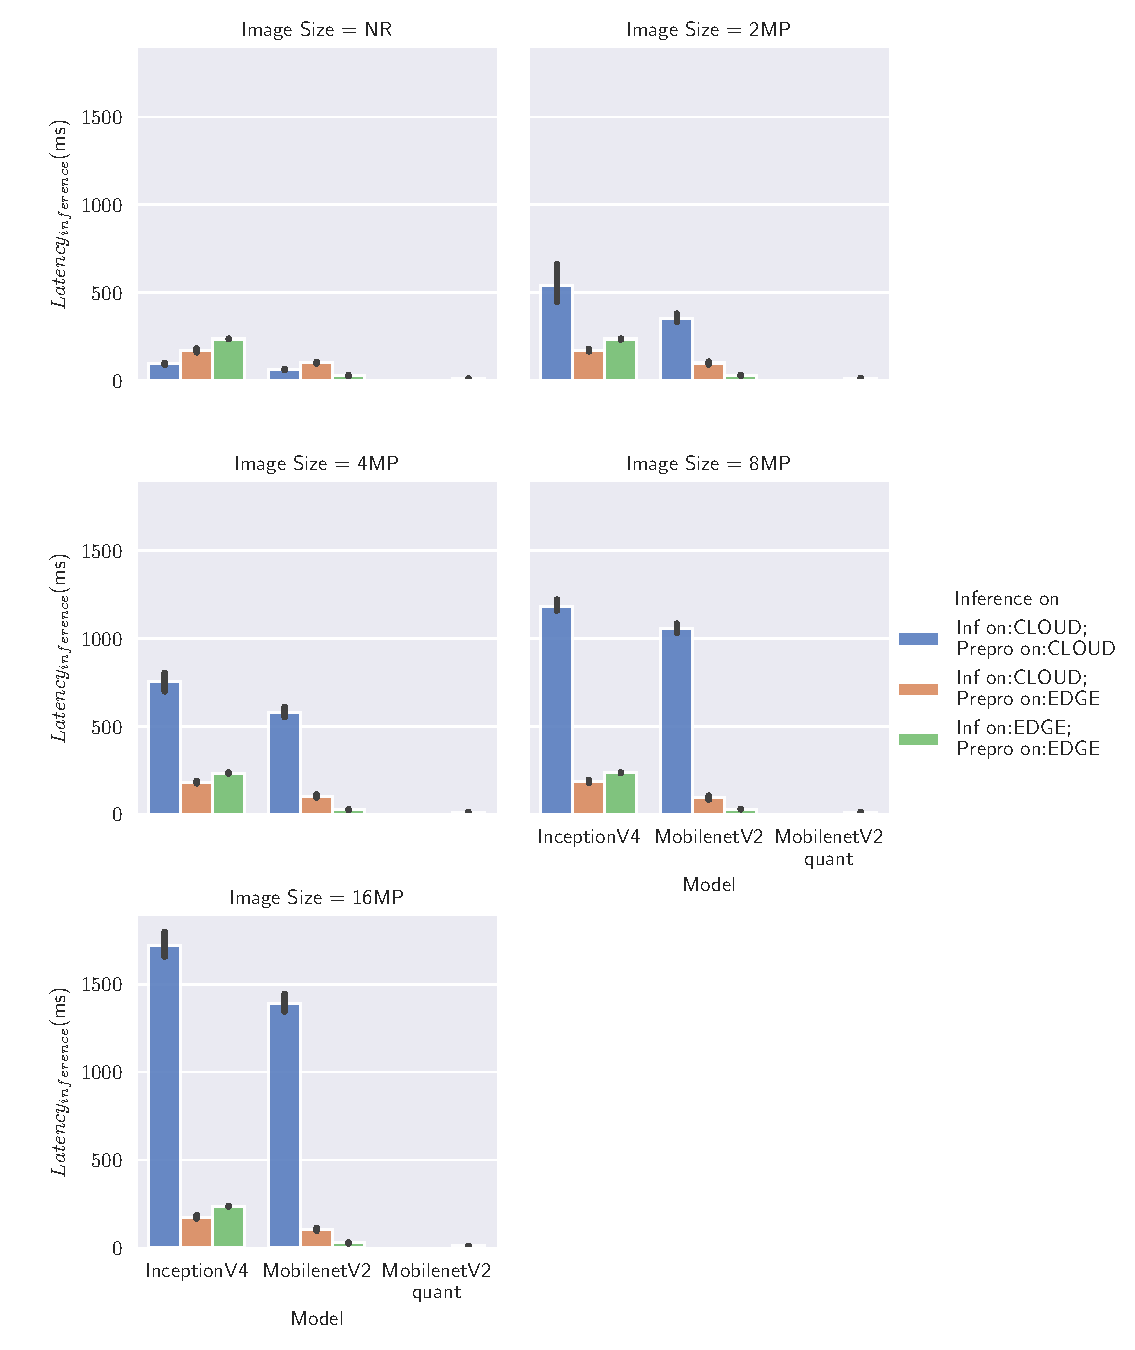
\includegraphics[width=0.95\textwidth]{./Bilder/single_plots/edge_vs_cloud_plots/Edge_vs_Cloud_Inference_Inference_Latencies.pdf}
\caption{Edge vs. Cloud Inference:  $Latency_{inference}$ - lower is better}
\label{fig:EdgeVsCloudInferenceLat}
\end{figure}

\begin{figure}[!htb]
\centering
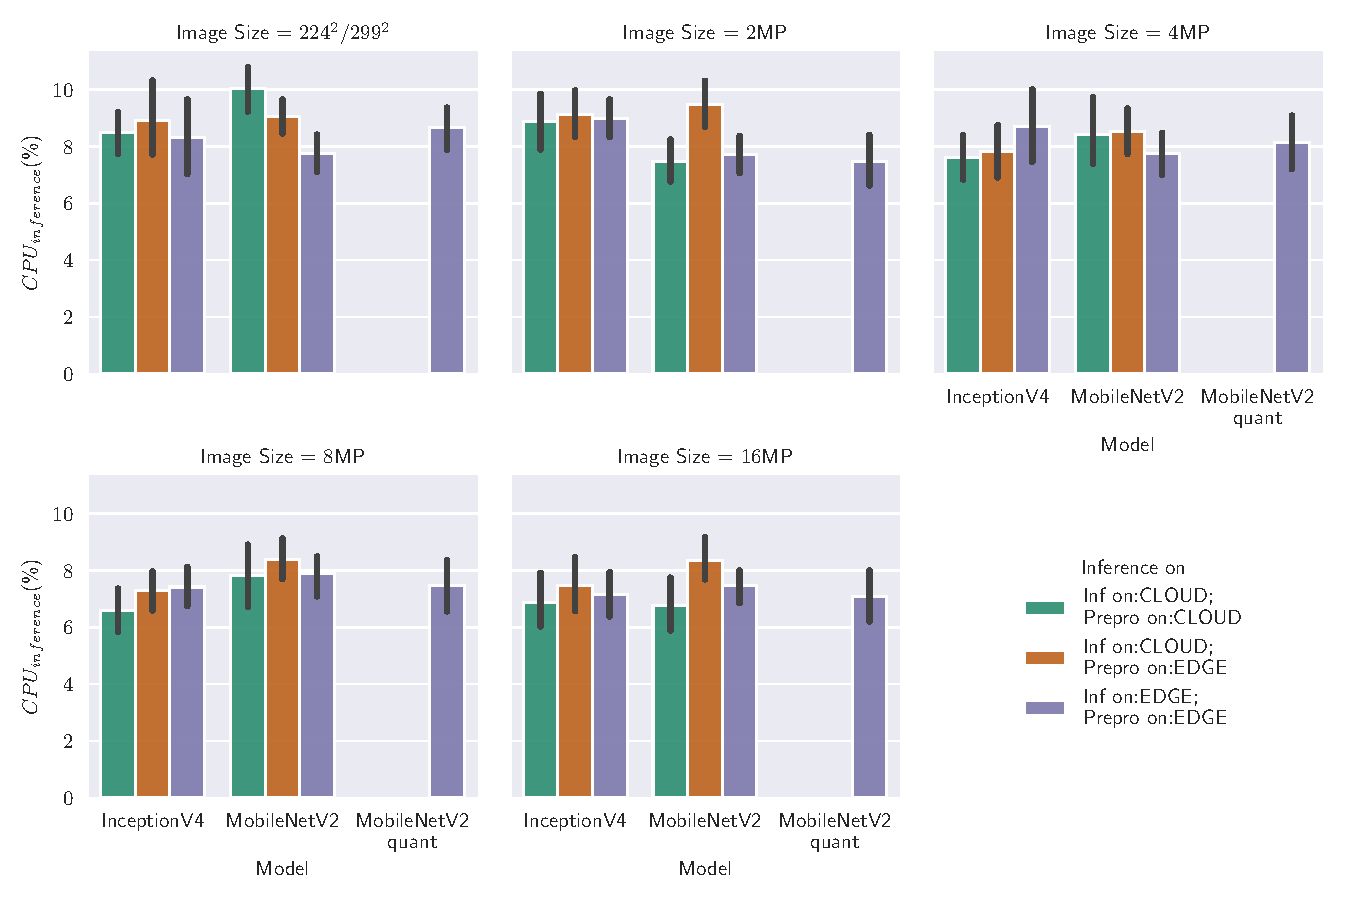
\includegraphics[width=0.95\textwidth]{./Bilder/single_plots/edge_vs_cloud_plots/Edge_vs_Cloud_Inference_Inference_CPU.pdf}
\caption{Edge vs. Cloud Inference:  $CPU_{inference}$ - lower is better}
\label{fig:EdgeVsCloudInferenceCPU}
\end{figure}


\begin{figure}[!htb]
\centering
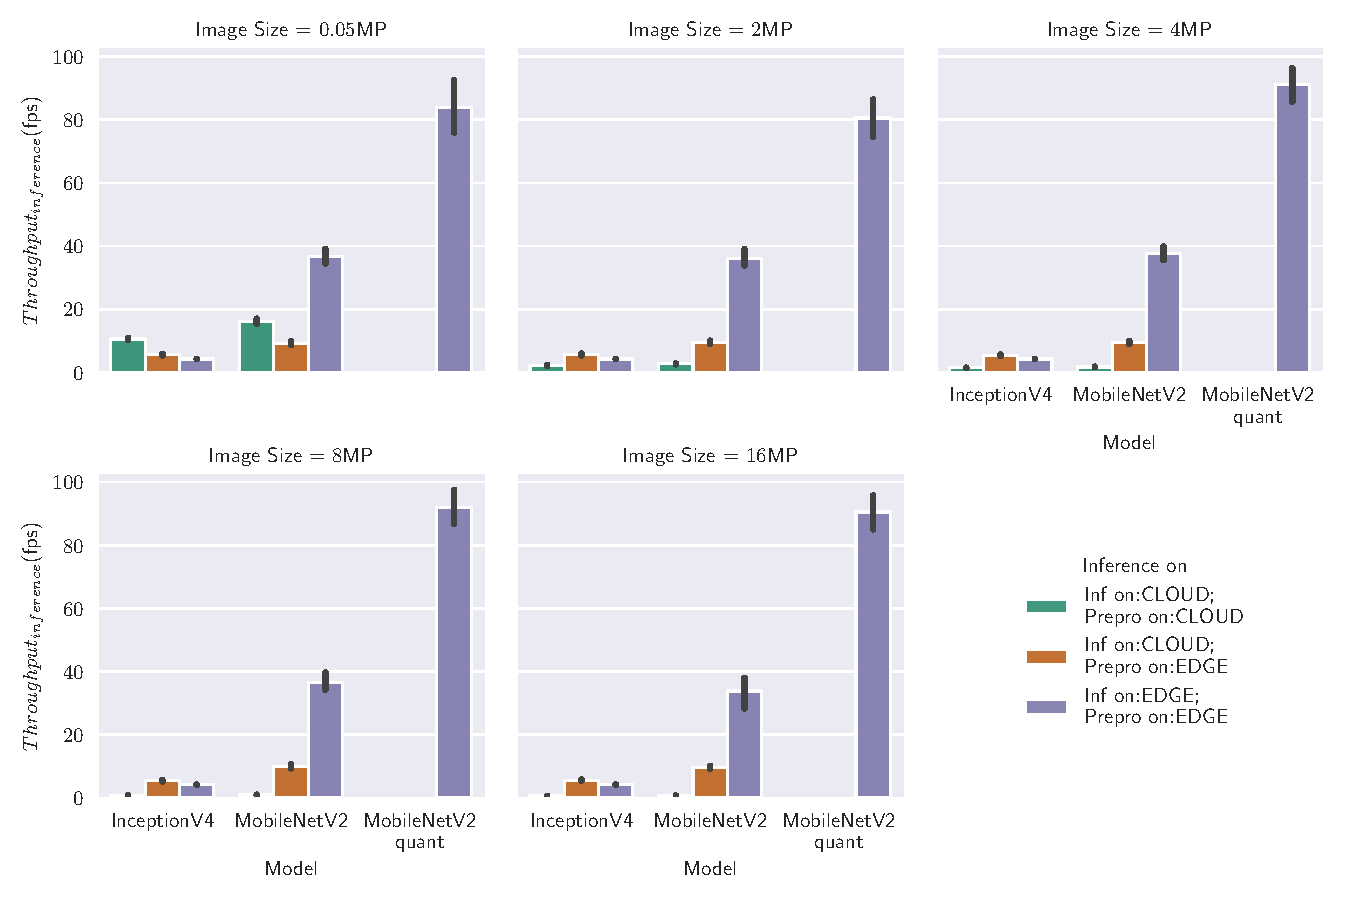
\includegraphics[width=0.95\textwidth]{./Bilder/single_plots/edge_vs_cloud_plots/Edge_vs_Cloud_Inference_Throughput_without_Preprocessing.pdf}
\caption{Edge vs. Cloud Inference:  $Throughput_{inference}$ - higher is better}
\label{fig:EdgeVsCloudinferneceThroughput}
\end{figure}

\begin{figure}[!htb]
\centering
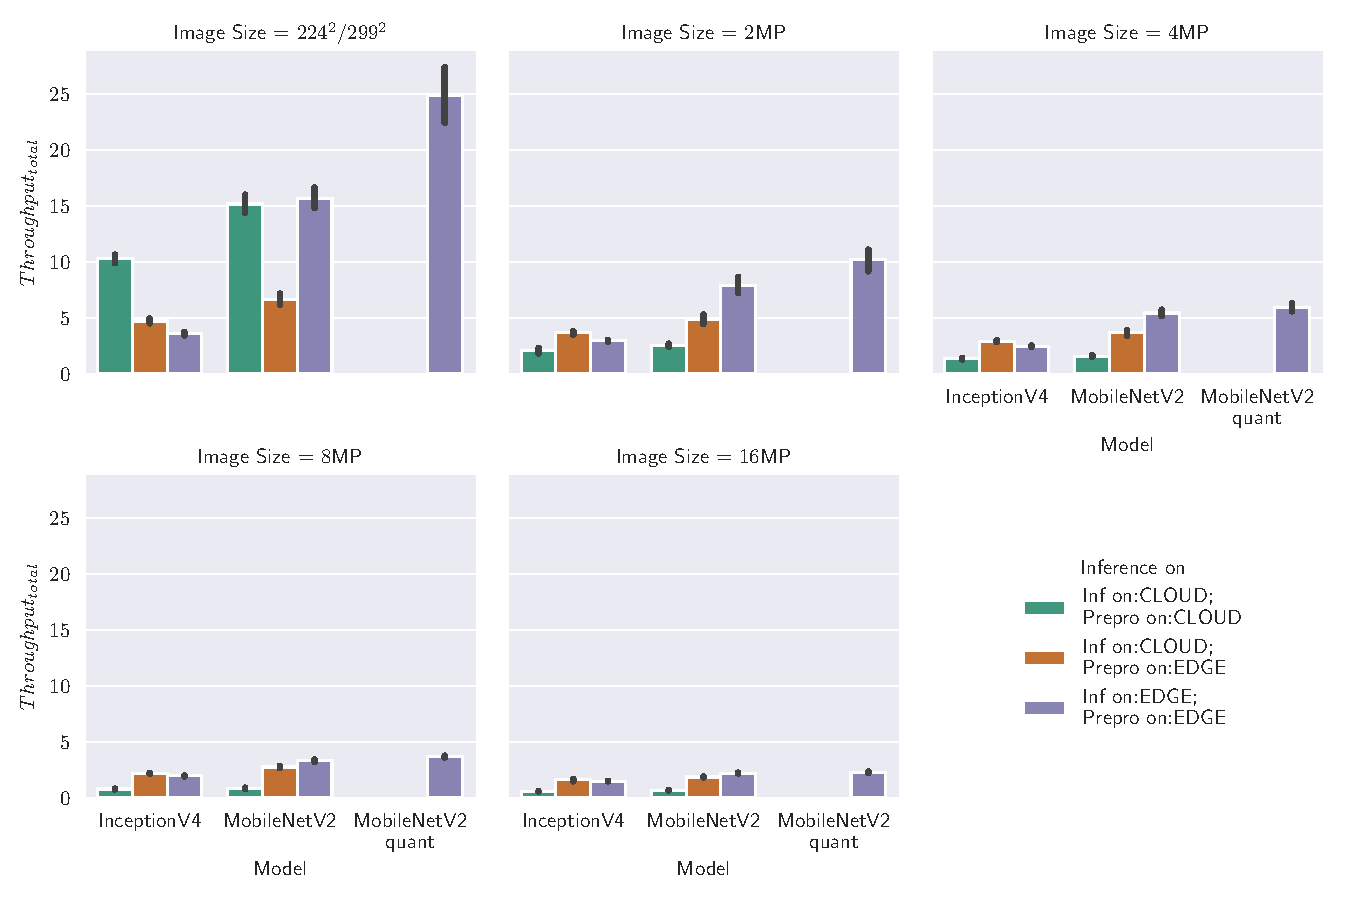
\includegraphics[width=0.95\textwidth]{./Bilder/single_plots/edge_vs_cloud_plots/Edge_vs_Cloud_Inference_Throughput_with_Preprocessing.pdf}
\caption{Edge vs. Cloud Inference:  $Throughput_{total}$ (Inference + Preprocessing) - higher is better}
\label{fig:EdgeVsCloudTotalThroughput}
\end{figure}



Concluding it can be stated that the edge is the preferred deployment option for MobileNetV2, both quantized and non quantized versions, in respect to latency/throughput as well as memory consumption.
The impact of I/O and network latency added by cloud inference is not feasible for these small models.

While the edge is the preferred for small models like MobileNetV2, InceptionV4's architecture is too demanding for the current edge devices, thus cloud inference is the better option for these large models.
Cloud preprocessing is only viable for the small $224^2/299^2$ images, as it lowers I/O costs and data consumption. For all other images sizes it increases $Latency_{total}$, $Data_{transmitted}$ and $Memory_{inference}$, while only having little positive effect on $Memory_{preprocessing}$ compared to the other inference options.

In general it can be stated that the impact of preprocessing is big, even for small images sizes, thus the preprocessing should be minimized as much as possible.


\paragraph{Edge vs. Cloud Inference - Key Takeaways}
\emph{
\subparagraph*{Preprocessing}
\begin{itemize}
    \item Both edge preprocessing methods for either edge or cloud inference are very similar in their preprocessing metrics.
    \item Cloud inference with cloud preprocessing compared to edge preprocessing options causes
    \begin{itemize}
        \item  (x for NR y for 16MP) less $Memory_{preprocessing}$ 
        \item (x for NR y for 16MP) faster $Latency_{preprocessing}$ 
        \item No significant differences in $CPU_{preprocessing}$
    \end{itemize}
    \item z
\end{itemize}
\subparagraph*{Inference}
\begin{itemize}
    \item x
    \item x
    \begin{itemize}
        \item  x
        \item x
        \item z
    \end{itemize}
    \item x
    \item z
\end{itemize}
\begin{itemize}[leftmargin=4em]
 \renewcommand{\labelitemi}{$\Rightarrow$}
 \item Edge inference performs better for small models, cloud inference performs better for large models.
 \item Preprocessing cost should be minimized as much as possible.
\end{itemize}
}
\FloatBarrier
\subsubsection{Effect of larger Batch Sizes}
\label{chap:resultsBatchSize}
So far we only reported the results of the of the experiments with batch size of one, but in this section we present the results for the batch sizes $1$, $2$, $16$, $32$.
Increasing the batch size  is supposed to increase throughput at the expense of low latencies.
Since the TensorFlow Lite of the used MobileNetV2 version does not allow batch sizes larger than one, we can not report edge inference results for these models.

Since the batch size is added as a new dimension in this section, the plots visualizing the results need to be expanded.
Now the x-axis represents the various batch sizes and the models are moved to the legend. 
The legend is similar to table \ref{table:legendPlots}, but the model is added as an additional feature to the inference mode.
\subsubsection{Preprocessing}

\paragraph{$\mathbf{CPU_{preprocessing}}$}
While the CPU usages for batch sizes of one were not different for the different deployment options, for larger batch sizes this changes, since in case of edge preprocessing the parallelism comes into play.
Recall that for batch sizes larger than one images get resized and normalized in parallel in the case of edge preprocessing to increase throughput (for implementation details refer to section \ref{chap:preproImpl}).

For rising images size and batch size the CPU usages rise up to $92\%$, as can be seen in figure \ref{fig:BatchSizePreproCPU}.

While CPU usages of the cloud preprocessing options also rise for increasing image/batch sizes, they stagnate at below $20\%$.
\begin{figure}[!htb]
\centering
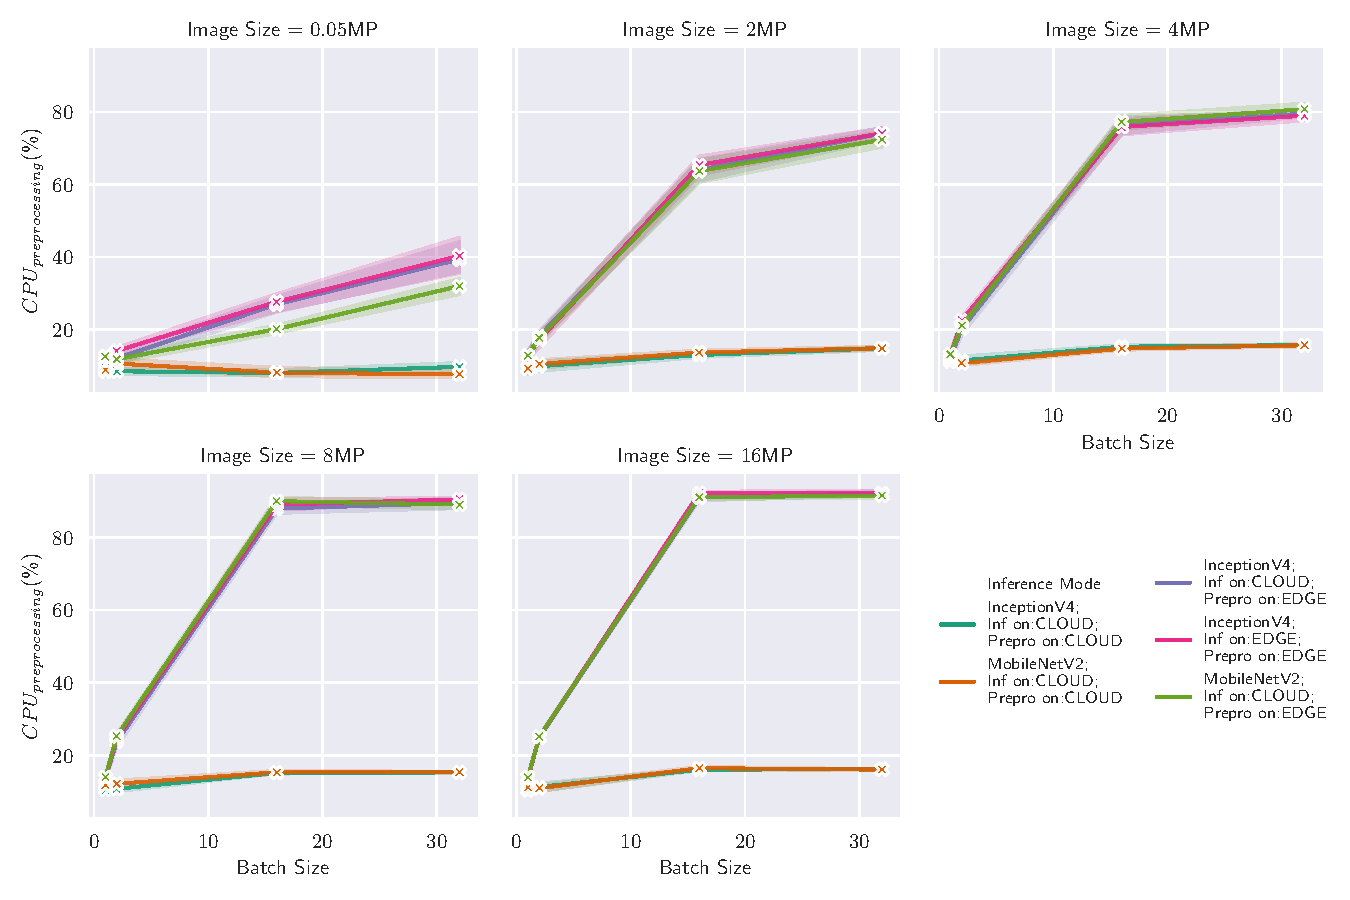
\includegraphics[width=0.95\textwidth]{./Bilder/single_plots/batch_size_plots/Effects_of_Batch_size_Preprocessing_CPU_Usage.pdf}
\caption{Edge vs. Cloud Inference for larger Batch Sizes -  $CPU_{preprocessing}$ - lower is better}
\label{fig:BatchSizePreproCPU}
\end{figure}

\paragraph{$\mathbf{Latency_{preprocessing}}$}
\begin{figure}[!htb]
\centering
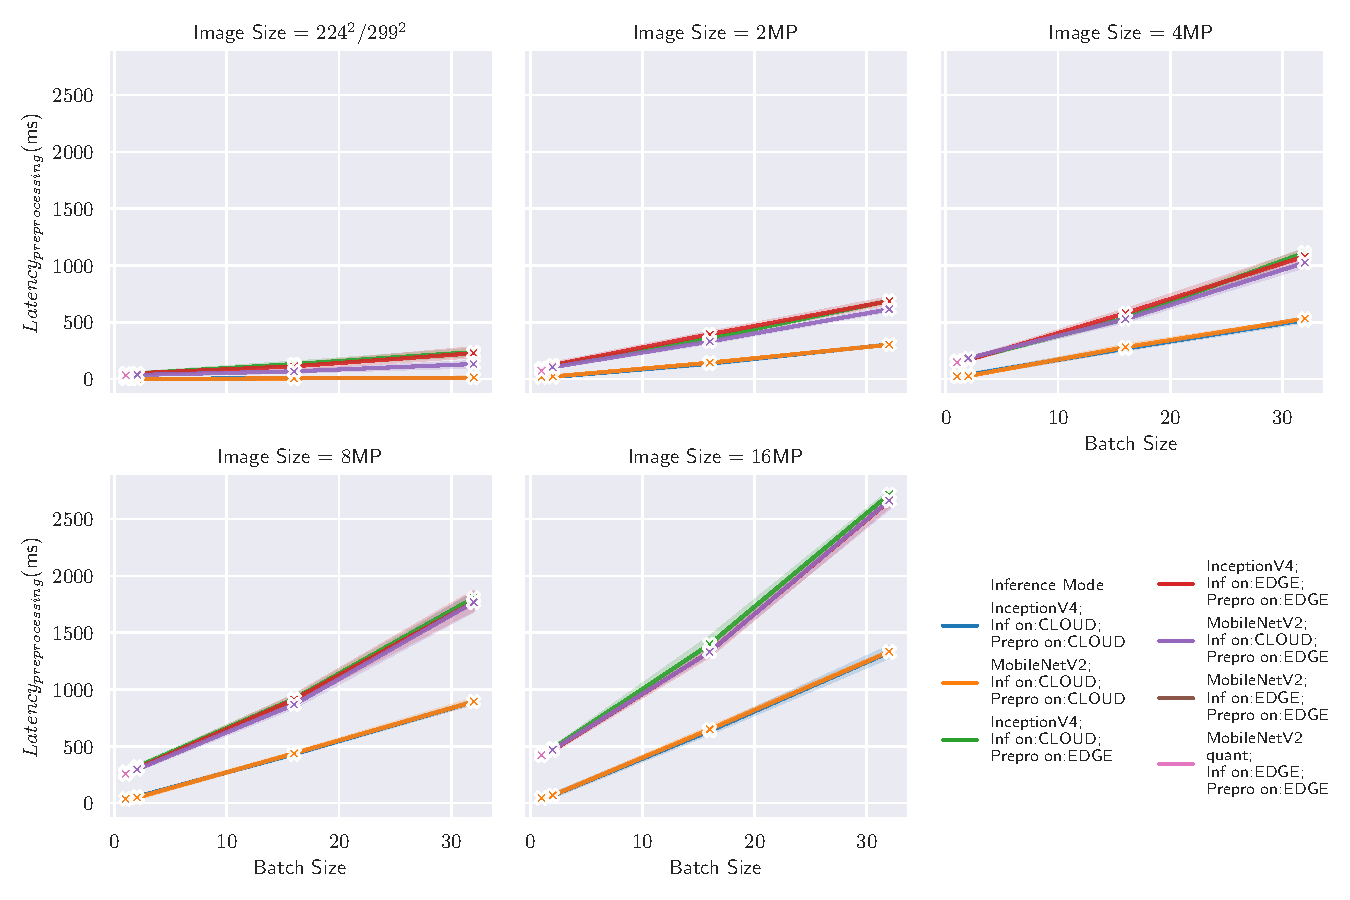
\includegraphics[width=0.95\textwidth]{./Bilder/single_plots/batch_size_plots/Effects_of_Batch_size_Preprocessing_Latencies.pdf}
\caption{Edge vs. Cloud Inference for larger Batch Sizes -  $Latency_{preprocessing}$ - lower is better}
\label{fig:BatchSizePreproLatency}
\end{figure}

\paragraph{$\mathbf{Memory_{preprocessing}}$}
\begin{figure}[!htb]
\centering
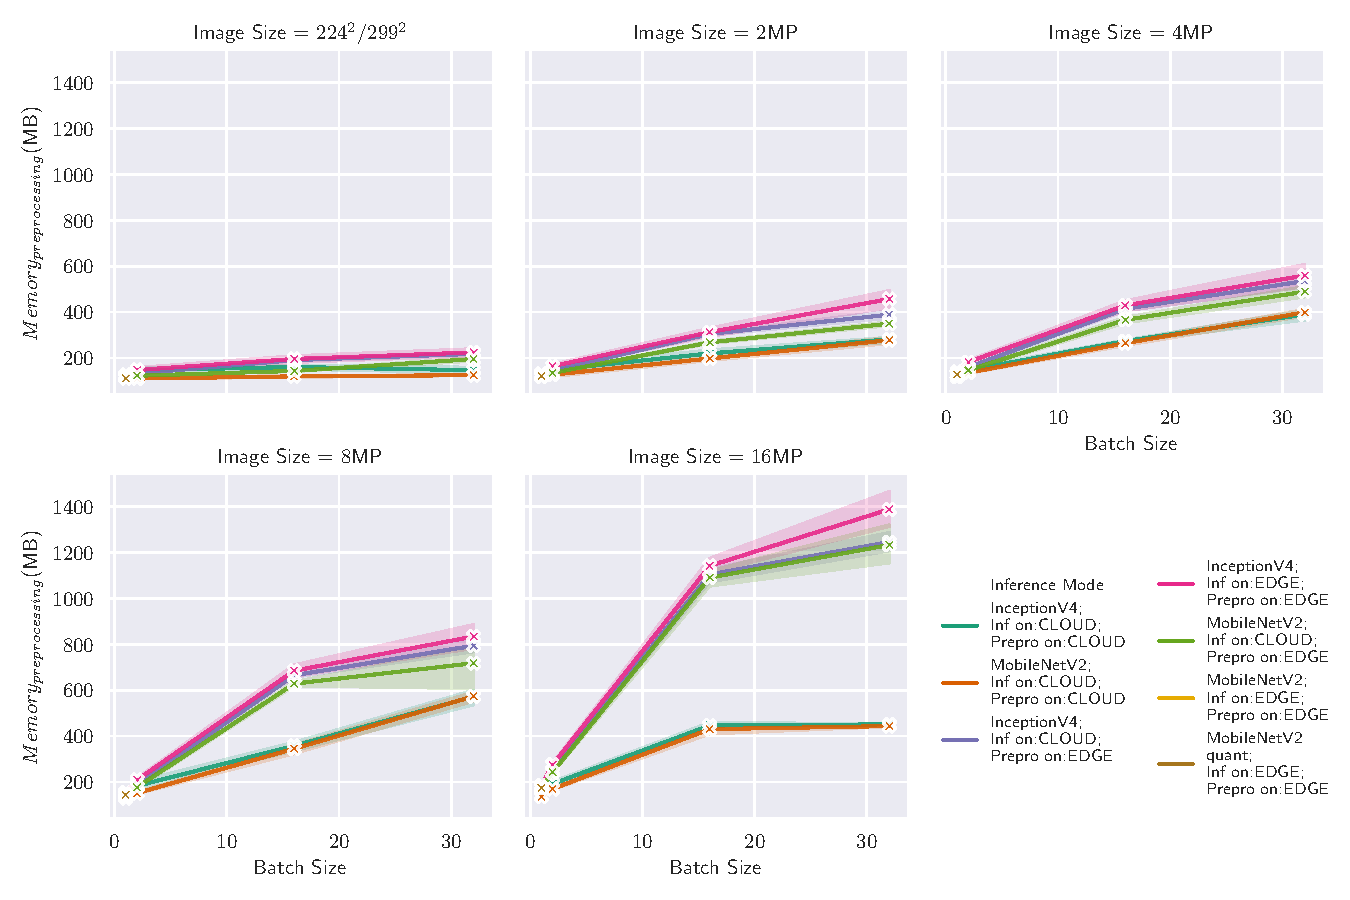
\includegraphics[width=0.95\textwidth]{./Bilder/single_plots/batch_size_plots/Effects_of_Batch_size_Preprocessing_Memory.pdf}
\caption{Edge vs. Cloud Inference for larger Batch Sizes -  $Memory_{preprocessing}$ - lower is better}
\label{fig:BatchSizePreproMemory}
\end{figure}

\FloatBarrier
\subsubsection{Inference}

\begin{figure}[!htb]
\centering
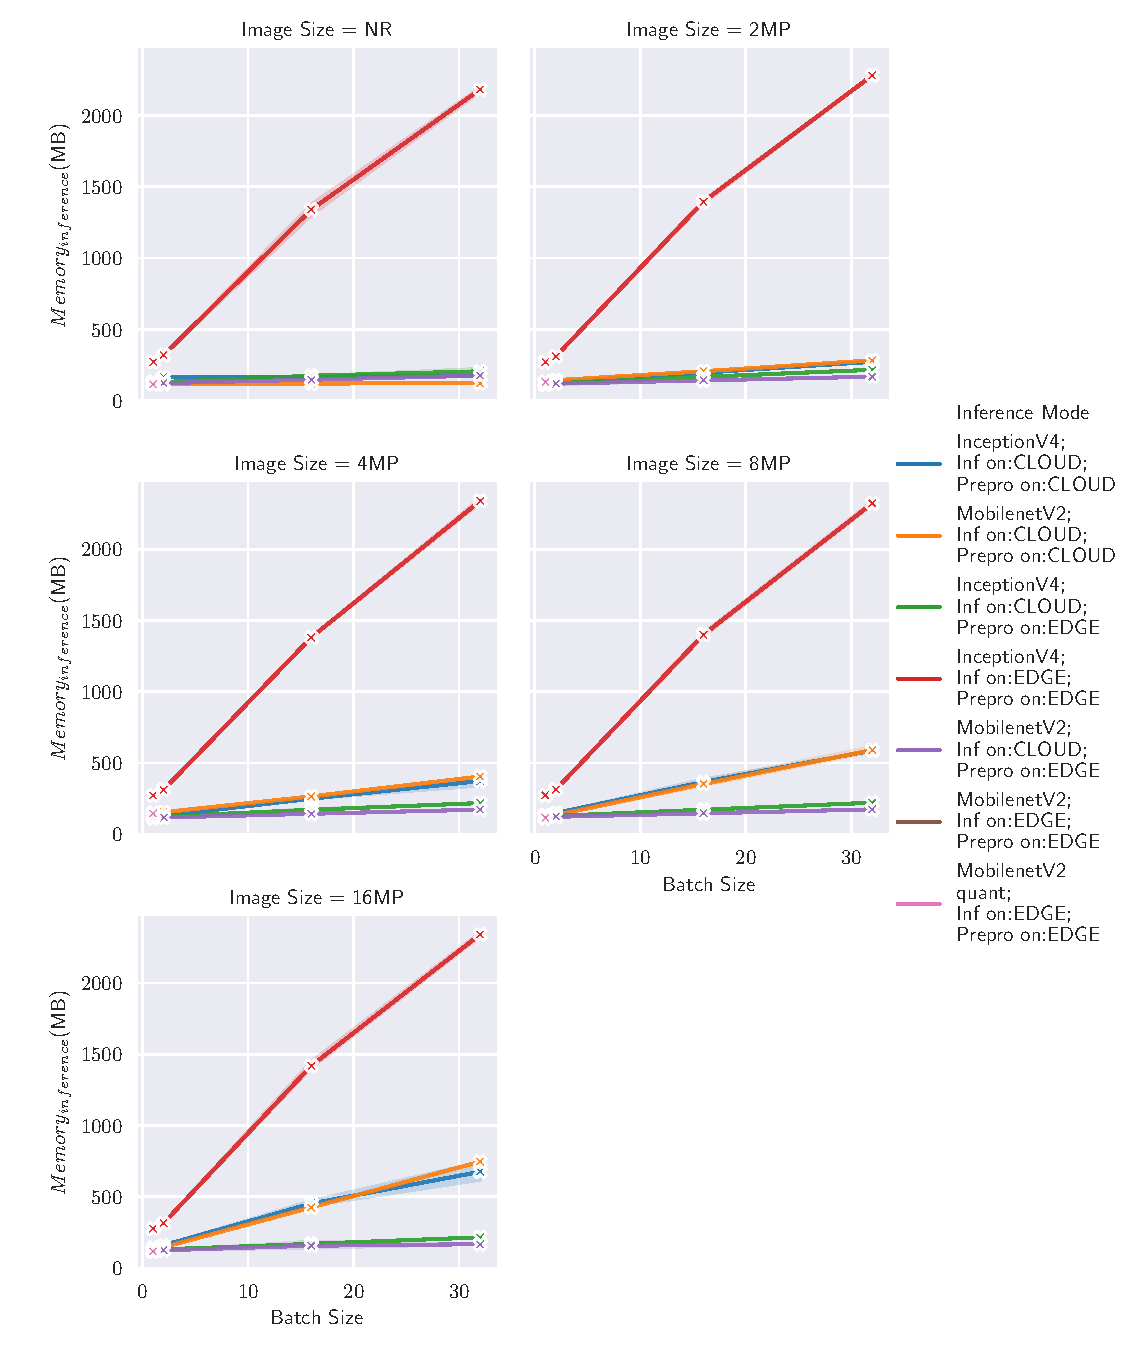
\includegraphics[width=0.95\textwidth]{./Bilder/single_plots/batch_size_plots/Effects_of_Batch_size_Inference_Memory.pdf}
\caption{Edge vs. Cloud Inference for larger Batch Sizes -  $Memory_{inference}$ - lower is better}
\label{fig:BatchSizeInferenceMemory}
\end{figure}
\begin{figure}[!htb]
\centering
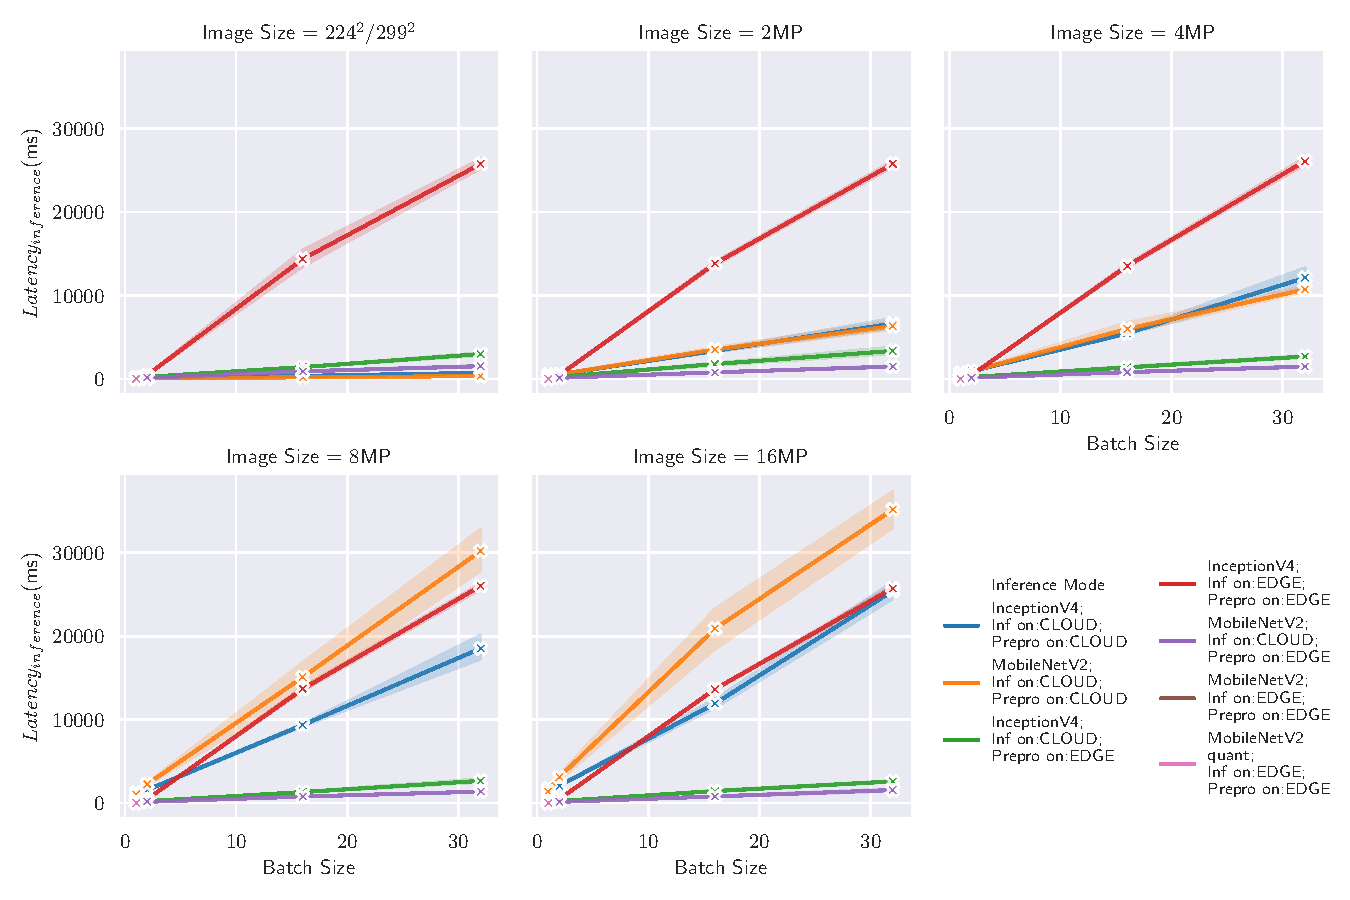
\includegraphics[width=0.95\textwidth]{./Bilder/single_plots/batch_size_plots/Effects_of_Batch_size_Inference_Latencies.pdf}
\caption{Edge vs. Cloud Inference for larger Batch Sizes -  $Latency_{inference}$ - lower is better}
\label{fig:BatchSizeInferenceLatency}
\end{figure}



\begin{figure}[!htb]
\centering
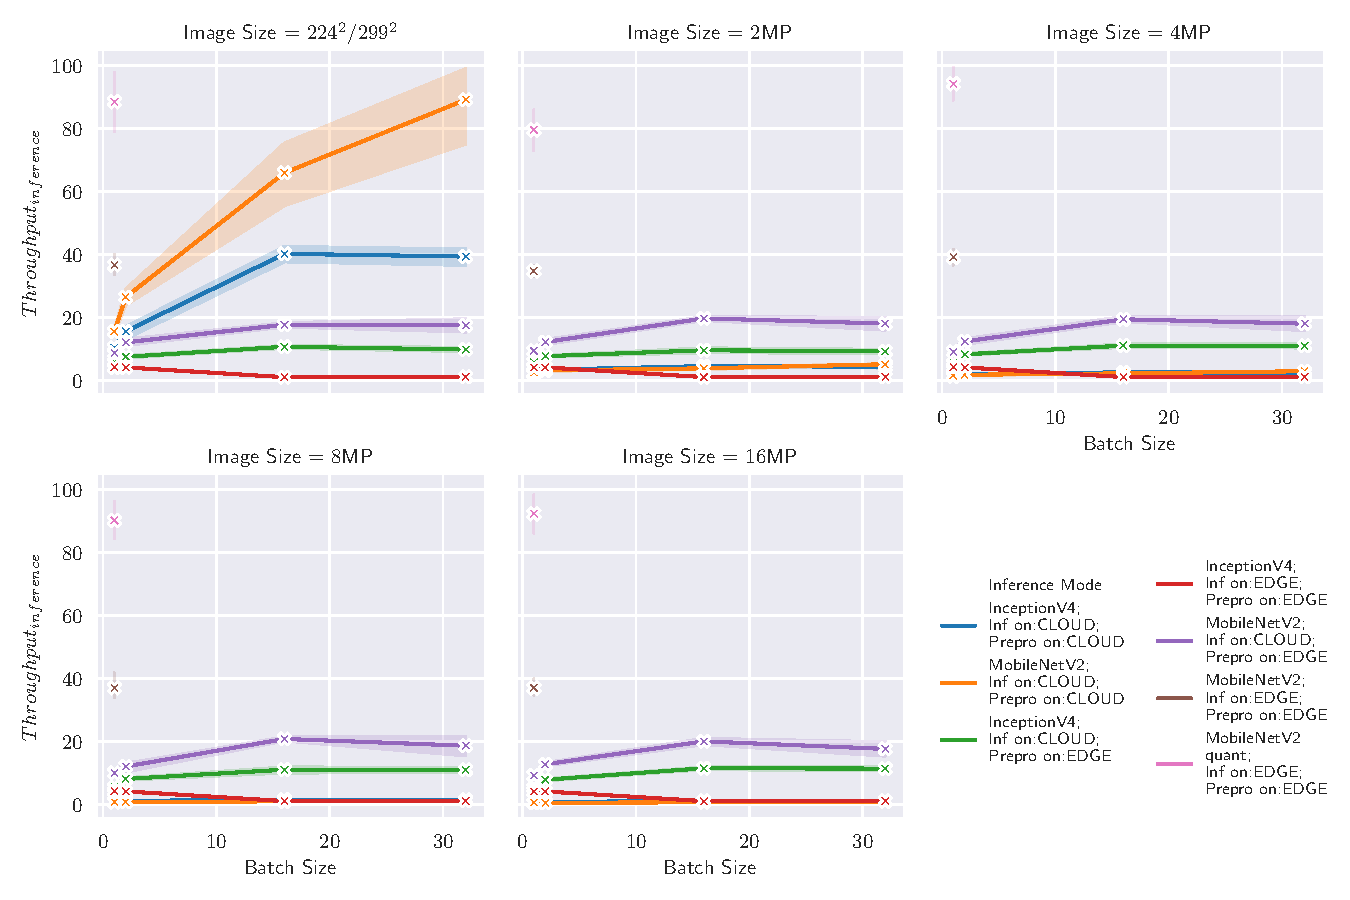
\includegraphics[width=0.95\textwidth]{./Bilder/single_plots/batch_size_plots/Effects_of_Batch_size_Inference_Throughput.pdf}
\caption{Edge vs. Cloud Inference for larger Batch Sizes -  $Throughput_{inference}$ - higher is better}
\label{fig:BatchSizeInferenceThroughput}
\end{figure}
\begin{figure}[!htb]
\centering
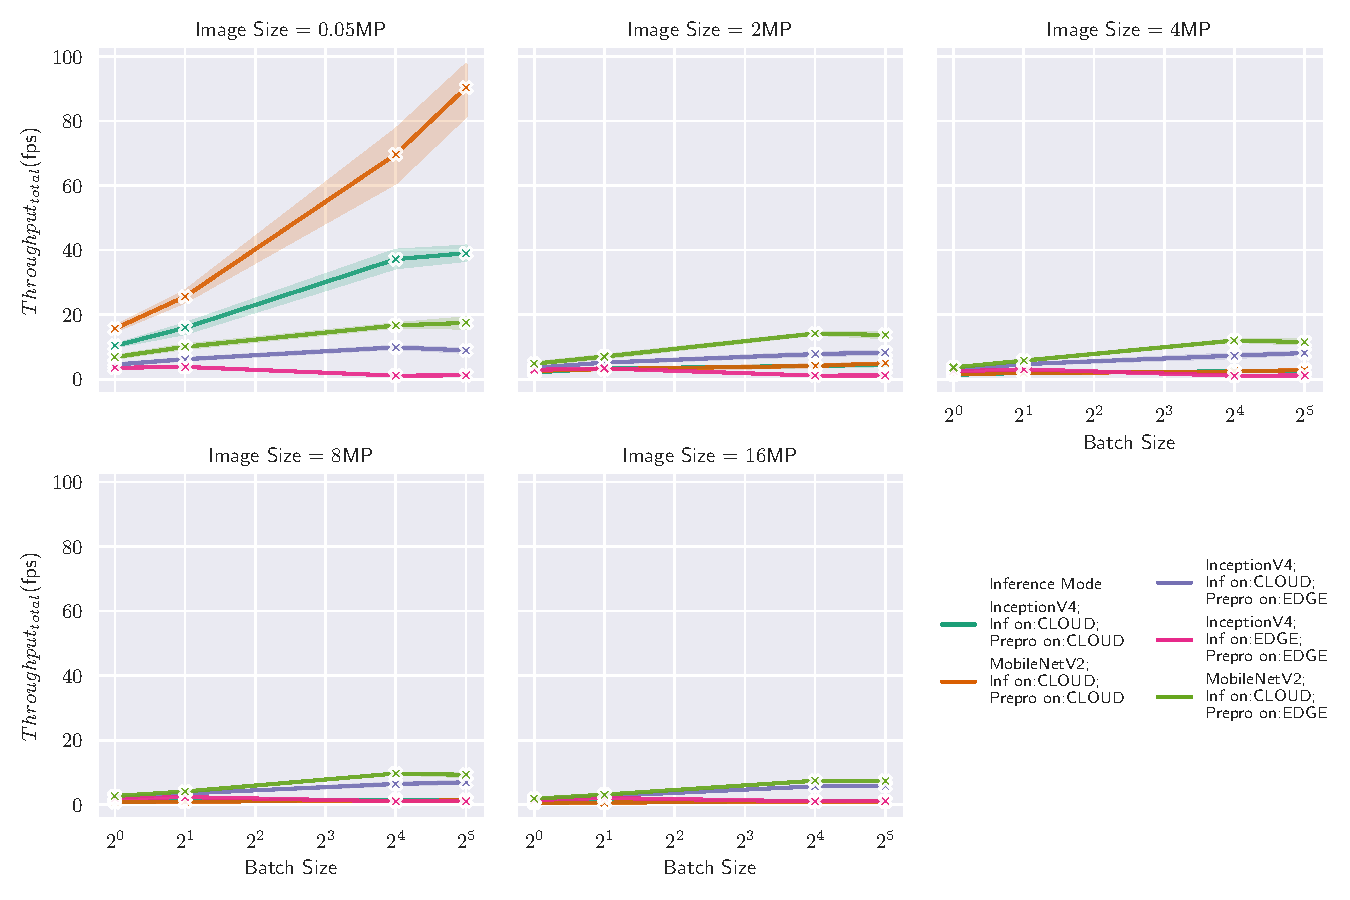
\includegraphics[width=0.95\textwidth]{./Bilder/single_plots/batch_size_plots/Effects_of_Batch_size_Total_Throughput_(Preprocessing_+_Inference).pdf}
\caption{Edge vs. Cloud Inference for larger Batch Sizes -  $Throughput_{total}$ - higher is better}
\label{fig:BatchSizeTotalThroughput}
\end{figure}


\FloatBarrier
%%throughput can be increase 
\paragraph{Effect of larger Batch Sizes - Key Takeaways}
\emph{
\subparagraph*{Preprocessing}
\begin{itemize}
    \item B
    \begin{itemize}
        \item  x
\end{itemize}
    \item x
\end{itemize}
\subparagraph*{Inference}
\begin{itemize}
    \item x
    \begin{itemize}
        \item  x
    \end{itemize}
    \item x
\end{itemize}
\begin{itemize}[leftmargin=4em]
 \renewcommand{\labelitemi}{$\Rightarrow$}
 \item Cloud inference throughput can be increased by increasing batch sizes, but not edge inference throughput
 \item Cloud inference outperforms edge inference for all model types for batch sizes larger than one
 \item Current edge devices not enough computational power for large batch sizes.
\end{itemize}
}


%%%%%%%%%%%%%%%%%%%%%%%%%
%Überleitung

\endinput 
